\documentclass{tufte-handout}

%--------Packages--------
\usepackage{booktabs,tabularx}
\usepackage{amsmath,amsthm,mathrsfs,bbm,blkarray}

%-------theorem Environments--------
\newtheorem{thm}{Theorem}
\newtheorem{cor}[thm]{Corollary}
\newtheorem{lem}[thm]{Lemma}
\newtheorem{defn}[thm]{Definition}
\newtheorem{rmk}[thm]{Remark}

%--------Colored Theorem-------------
\usepackage[most]{tcolorbox}
\definecolor{baby-pink}{cmyk}{0,0.95,0.0, 0,0}
\tcbuselibrary{theorems}
\newtcbtheorem
  []%
  {ex}
  {\textbf{Example}}
  {%
  	breakable,
    colback=baby-pink!5,
    colframe=baby-pink!85,
    fonttitle=\bfseries,
  }% options
  {def}% prefix

%--------Shortcuts--------
\usepackage{graphicx}
\graphicspath{{./figures/}}

\newcommand{\floor}[1]{\left\lfloor #1 \right\rfloor}
\newcommand{\ceil}[1]{\left\lceil #1 \right\rceil}

%--------Header--------
\title{W2022-MATH447: Stochastic Processes}
\author[Jana Kurrek]{Jana Kurrek \vfill}
\date{\today}

%--------Title--------
\makeatletter
\renewcommand{\maketitlepage}{
    \cleardoublepage{
        \begin{fullwidth}
        % \fontsize{12}{12}\selectfont\par\noindent{\@author \\ \noindent \small{Instructors: Paquette, Elliot }}
        \fontsize{12}{12}\selectfont\par\noindent{\@author \\ \noindent \small{\textbf{Lectures}: Paquette, Elliot } \\ \noindent \small{\textbf{Textbook}: Dobrow, Robert} \\}
        \vfill
        \vfill
        \fontsize{36}{40}\selectfont\par\noindent{Stochastic Processes}
        \vfill
		    \vspace{2pc}
        \noindent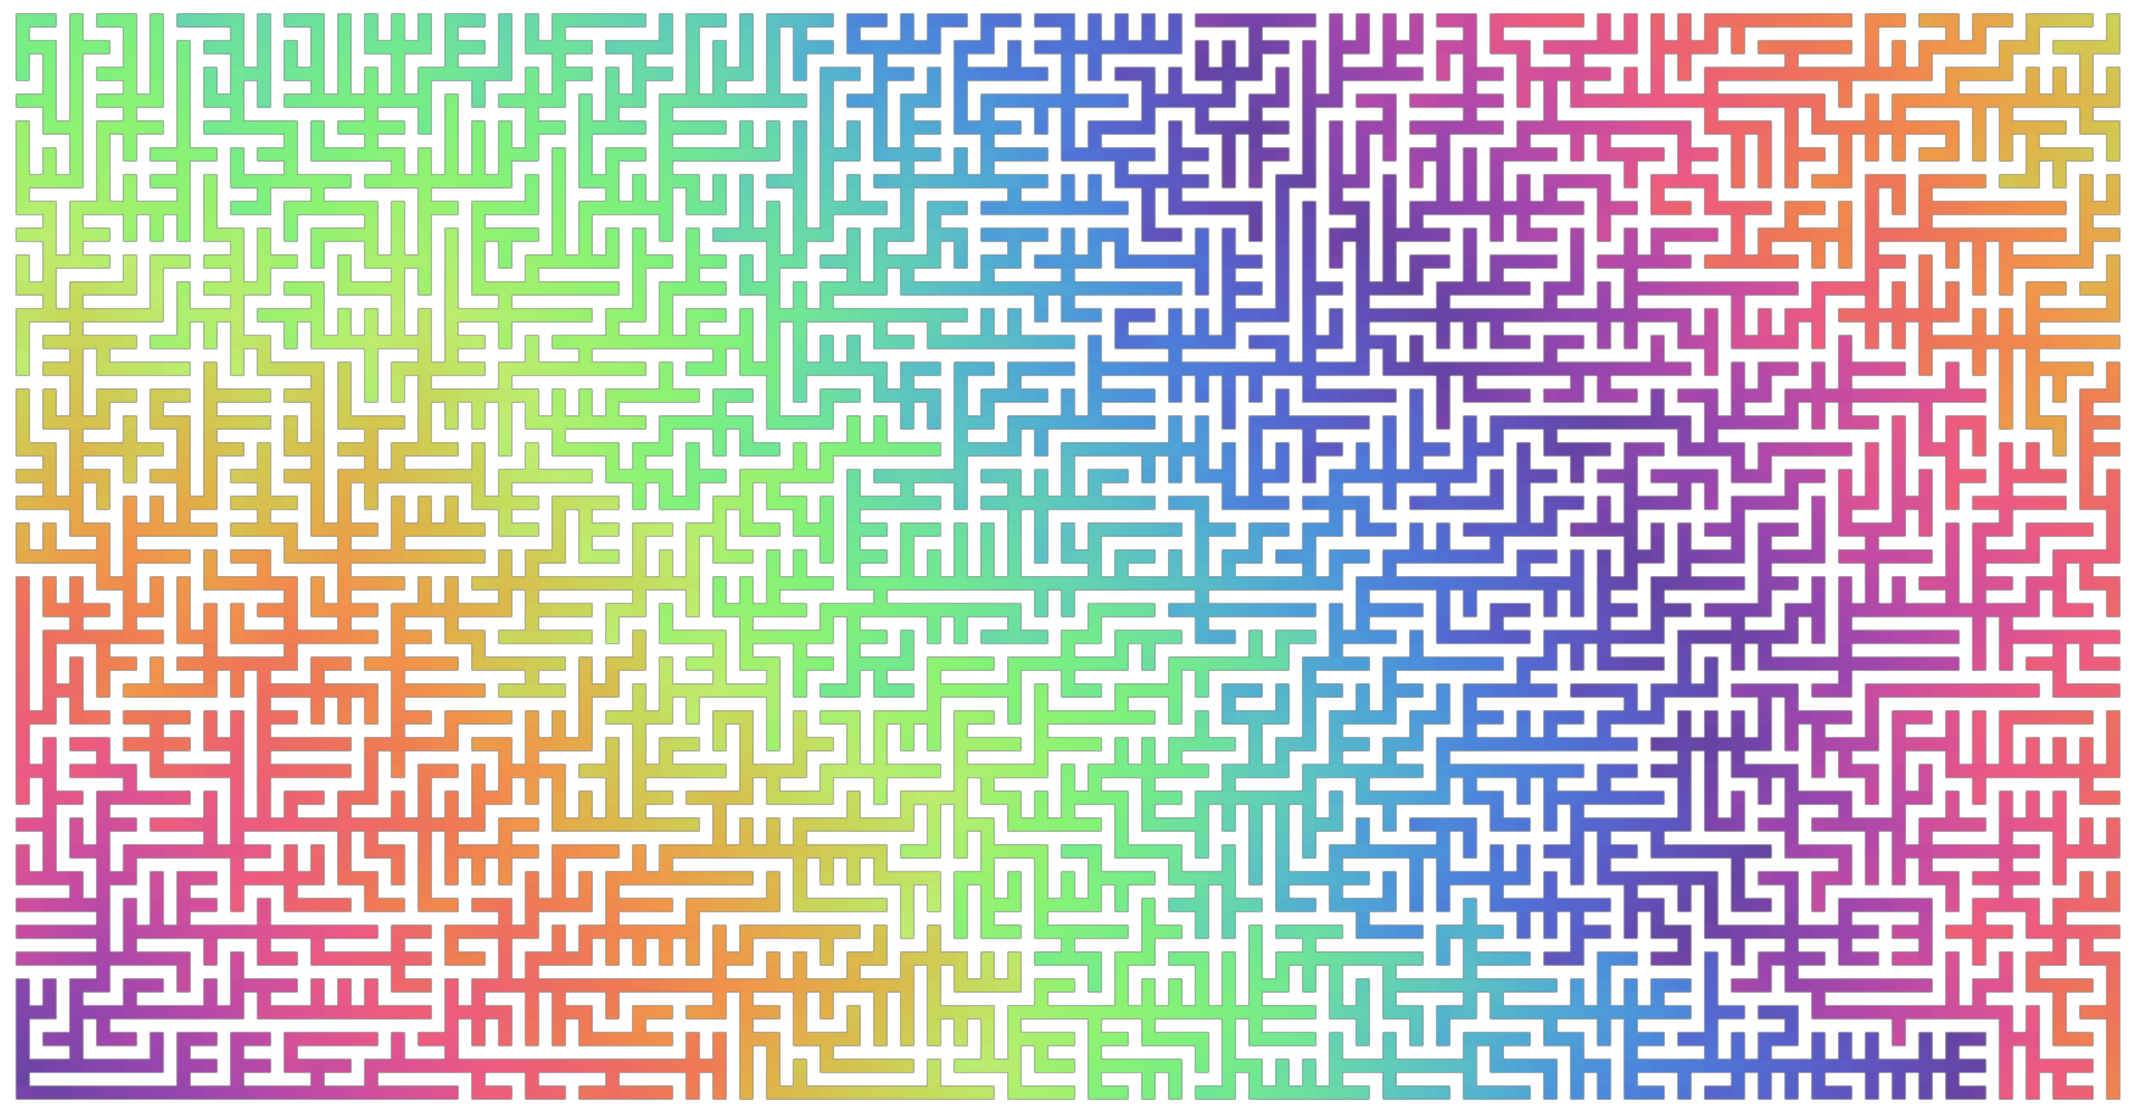
\includegraphics[width=1.5\textwidth]{title.png}
        \vspace{1pc}
		    \fontsize{10}{12}\selectfont\par\noindent{\textbf{Figure 1.} A uniform spanning tree of a rectangular box in the square grid $\mathbb{Z}^2$. Colours represent the distance to the bottom left corner modulo some constant. Image taken from Tom Hutchcroft.}
    		\vfill
        \vspace{15pc}
        \vfill
        \fontsize{10}{12}\selectfont\par\noindent{\textbf{Contents.} Conditional expectation; Generating functions; Branching processes and random walk; Markov chains, transition matrices, classification of states, ergodic theorem; Birth and death processes; Queueing.}
        \end{fullwidth}}
        \thispagestyle{empty}
        \clearpage
}
\makeatother

\begin{document}

% Title Page and Table of Contents
\maketitlepage
\tableofcontents
\newpage

% Conditional Expectation
\section{Axioms of Probability}
\subsection{Conditional Probability}
\begin{defn}[Conditional Probability]
  The \textbf{conditional probability of $A$ given $B$}, defined for $P(B) > 0$, is,
  \[P(A \text{ $|$ } B) = \frac{P(A \cap B)}{P(B)}\]
\end{defn}

\begin{defn}[Independence]
  Events $A$ and $B$ are \textbf{independent} if $P(A \text{ $|$ } B) = P(A)$. Equivalently, $P(A \cap B) = P(A) P(B)$.
\end{defn}

\begin{defn}[Total Law of Probability]
  Let $B_1, \cdots, B_k$ be a sequence of events that partition $\Omega$. Then, for any event $A$,
  \[P(A)=P\left(\bigcup_{i \in [k]}\left(A \cap B_{i}\right)\right)=\sum_{i}^k P\left(A \cap B_{i}\right)=\sum_{i}^k P\left(A \mid B_{i}\right) P\left(B_{i}\right)\]
  \noindent More generally, $P(A) = \mathbb{E}[P(A \text{ $|$ } X)]$.
\end{defn}

\begin{defn}[Bayes' Rule]
  For events $A$ and $B$\footnote{With the Total Law of Probability, \[P\left(B_{i} \mid A\right)=\frac{P\left(A \mid B_{i}\right) P\left(B_{i}\right)}{\sum_{j} P\left(A \mid B_{j}\right) P\left(B_{j}\right)}\]},
  \[P(A \text{ $|$ } B)=\frac{P(B \text{ $|$ } A) P(A)}{P(B)}\]
\end{defn}

\subsection{Conditional Distributions}
\begin{defn}[Conditional Probability Mass Function]
  The \textbf{conditional probability mass function of $Y$ given $X = x$} is,
  \[P(Y=y \mid X=x)=\frac{P(X=x, Y=y)}{P(X=x)}\]
\end{defn}

\begin{defn}[Conditional Probability Density Function]
  The \textbf{conditional probability density function of $Y$ given $X = x$} is,
  \[f_{Y|X}(y|y) = \frac{f(x,y)}{f_X(x)}\]
\end{defn}

\subsection{Conditional Expectation}
\begin{defn}[Conditional Expectation]
  The \textbf{conditional expectation of $Y$ given $X = x$}, written $\mathbb{E}[Y \text{ $|$ } X = x](x)$, is a function of $x$,
  \[
  \mathbb{E}[Y \text{ $|$ } X = x](x) = \begin{cases}
    \sum_{y} y \cdot P(Y = y \text{ $|$ } X = x) & \text{$\Omega$ is discrete} \\
    \int_{-\infty}^{\infty} y \cdot f_{Y \mid X}(y \mid x) d y & \text{$\Omega$ is continous}
  \end{cases} 
  \]
\end{defn}

\begin{marginfigure}
  \textbf{Summary of Conditional Probability:}
  \begin{itemize}
      \item Total Probability
      \[P(A) = \mathbb{E}[P(A \text{ $|$ } X)]\]
      \item Total Expectation
      \[\mathbb{E}[Y] = \mathbb{E}[\mathbb{E}[Y \text{ $|$ } X]]\]
      \item Total Conditional Expectation
      \[P(Y \text{ $|$ } A) = \mathbb{E}[P(Y \text{ $|$ } X, A) \text{ $|$ } A]\]
      \item Total Conditional Probability
      \[\mathbb{E}[Y \text{ | } A] = \mathbb{E}[\mathbb{E}[Y \text{ | } X,A] \text{ | } A]\]
  \end{itemize}
\end{marginfigure}

\begin{defn}
  The \textbf{conditional expectation of $Y$ given $A$} is,
  \begin{align*}
    E(Y \mid A)&=\frac{1}{P(A)} \sum_{y} y P(\{Y=y\} \cap A) \\
               &=\sum_{y} y P(Y=y \mid A)
  \end{align*}
  \noindent for the discrete case.
\end{defn}

\begin{defn}[Law of Total Expectation]
  If $A_1, \cdots, A_k$ partitions $\Omega$ and $Y$ is a random variable, then the \textbf{law of total expectation} states that,
  \[\mathbb{E}[Y] = \sum_{i=1}^k \mathbb{E}[Y \text{ $|$ } A_i] P(A_i)\]
  \noindent More generally, $\mathbb{E}[Y] = \mathbb{E}[\mathbb{E}[Y \text{ $|$ } X]]$.
\end{defn}

\begin{proof}
  For the discrete case, \begin{align*} \mathbb{E}[\mathbb{E}[Y \mid X]] &=\sum_{x} \mathbb{E}[Y \mid X=x] \cdot P(X=x) \\ &=\sum_{x}\left(\sum_{y} y P(Y=y \mid X=x)\right) P(X=x) \\ &=\sum_{y} y \sum_{x} P(Y=y \mid X=x) \cdot P(X=x) \\ &=\sum_{y} y \sum_{x} P(X=x, Y=y) \\ &=\sum_{y} y \cdot P(Y=y) \\ &=\mathbb{E}(Y) \end{align*}
\end{proof}

\section{Time-Homogeneous Markov Chains}
\subsection{Finite State, Time-Homogeneous Chains}
\begin{defn}[Finite State Stochastic Process]
    A \textbf{finite state stochastic process} $(X_n)_{n \geq 0}$ has time steps in $\mathbb{N}$ and values in $S = [N - 1]$.
  \end{defn}

  \begin{defn}[Markov Property]
    The \textbf{Markov property} claims that for every $n \in \mathbb{N}$ and every sequence of states $(i_0, i_1, \cdots)$ where $i_j \in S$, the behavior of a system depends only on the previous state,
    \[
    P(X_n = i_n \text{ $|$ } X_0 = i_0, \cdots, X_{n-1} = i_{n-1}) = P(X_n = i_n \text{ $|$ } X_{n-1} = i_{n-1})
    \]
  \label{markovprop}
  \end{defn}

  \begin{defn}[Time Homogeneity]
  A Markov chain is \textbf{time-homogeneous} if the probabilities in Definition \ref{markovprop} do not depend on $n$,
  \[
    P(X_n = i_n \text{ $|$ } X_{n-1} = i_{n-1}) = P(X_1 = i_1 \text{ $|$ } X_0 = i_0) \quad (n \in \mathbb{N})
  \]
  \end{defn}

  \begin{defn}[Transition Matrix]
    The \textbf{transition matrix} $\boldsymbol{P}$ for a time-homogeneous Markov chain is the $N \times N$ matrix whose $(i,j)$th entry $\boldsymbol{P}_{ij}$ is the one-step transition probability $p(i,j) = P(X_1 = j \mid X_0 = i)$.
  \end{defn}

  \begin{rmk}
     The transition matrix $\boldsymbol{P}$ is stochastic, that is,
      \begin{itemize}
        \item (Non-Negative Entries) $0 \leq \boldsymbol{P}_{ij} \leq 1$ for $1 \leq i,j \leq N$
        \item (Row Sum Equal to 1) $\sum_{j=1}^N \boldsymbol{P}_{ij} = 1$ for $1 \leq i \leq N$
      \end{itemize}
  \end{rmk}


  \begin{ex}{Biased Coin Flips}{label}
  Let $(X_n)_{n \geq 0}$ denote a sequence of coin flips where,
    \[P(X_{n+1} = H \text{ $|$ } X_n) = 
    \begin{cases}
        0.51 \text{ if  } X_n = H\\
        0.49 \text{ if } X_n  = T
    \end{cases}
    \]
    \noindent and,
    \[
    P(X_{n+1} = T \text{ $|$ } X_n) = 
    \begin{cases}
        0.51 \text{ if  }X_n = T\\
        0.49 \text{ if }X_n = H
    \end{cases}
    \]
    Then,
    \[\boldsymbol{P} = \begin{pmatrix}
    0.51 & 0.49\\ 0.49 & 0.51
    \end{pmatrix}  = \begin{pmatrix}
    P_{HH} & P_{HT}\\
    P_{TH} & P_{TT}
    \end{pmatrix} \]
  \end{ex}

  \subsection{Transition Probabilities}
  \begin{defn}[Probability Distribution Vector]
    The \textbf{distribution} of a discrete random variable $X$ is the vector $\Vec{\phi}$ if,
    \[\phi_{j} = P(X = j) \quad \text{$\forall j \in \mathbb{N}$}\]
  \end{defn}

  \begin{defn}[Initial Distribution Vector]
    The \textbf{initial probability distribution} of a Markov chain $(X_n)_{n \geq 0}$ is the distribution $\Vec{\phi}$ of $X_0$.
  \end{defn}

  \begin{thm}[Transition Probabilities]
    The $n$-step transition probability $p_n(i,j) = P(X_n = i \mid X_0 = j)$ is the $(i,j)$th entry in the matrix $\boldsymbol{P}^n$.
  \end{thm}

  \begin{proof}
  The base case is trivially true for $n = 1$. Assume the statement holds for a given $n$. Using the properties of matrix multiplication and the Law of Total Conditional Expectation,
  \begin{align*}
    P(X_{n+1} = j \text{ $|$ } X_0 = i)
    &= \sum_{k \in S} P(X_{n} = k \text{ $|$ } X_0 = i) \cdot P(X_{n+1} = j \text{ $|$ } X_n = k) \\
    &= \sum_{k \in S} p_n(i,k) \cdot p(k,j) \\ 
    &= \boldsymbol{P}^n\boldsymbol{P} \\
    &= \boldsymbol{P}^{n+1}
  \end{align*}
  \end{proof}

  \begin{thm}[Chapman-Kolmogorov]
    Let $x,y,z \in S$ and $m, n \in (0, \infty)$.
    \begin{align*}
      p_{m+n}(x,y) &= P(X_{m+n} = y \text{ $|$ } X_0 = x) \\
      &= \sum_{z \in S}P(X_{m+n} = y, X_m = z \text{ $|$ } X_0 = x) \\
      &= \sum_{z \in S}p_m(x,z) \cdot p_n(z,y)
    \end{align*}
  \end{thm}

  \begin{marginfigure}
    The probabilistic interpretation for \textbf{Chapman-Kolmogorov} is that transitioning from $x$ to $y$ in $m + n$ steps is equivalent to transitioning from $i$ to $k$ in $m$ steps and then moving from $k$ to $j$ in the remaining $n$ steps.
  \end{marginfigure}

  \begin{defn}[Distribution of $X_n$]
    The \textbf{distribution of $(X_n)_{n \geq 0}$} is,
    \[\phi \cdot \boldsymbol{P}^n \quad \text{i.e., } P(X_n = j) = (\phi \cdot \boldsymbol{P}^n)_{j} \quad \forall j \in \mathbb{N}\]
    \noindent where $\boldsymbol{P}$ is the transition matrix of $(X_n)$ and $\phi$ is the initial distribution.
  \end{defn}

  \subsection{Stationary Distributions}
  \begin{defn}[Limiting Distribution Vector]
    A \textbf{limiting distribution} for a time-homogeneous Markov chain $(X_n)_{n \geq 0}$ is a distribution $\Vec{\pi}$ so that,
    \[\lim_{n \rightarrow \infty} p_n(i,j) = \pi_j\]
    \noindent The definition of a limiting distribution is equivalent to,
    \begin{itemize}
      \item $\lim_{n \rightarrow \infty} P(X_n = j) = \pi_j$
      \item $\lim_{n \rightarrow \infty} \Vec{\phi} \cdot \boldsymbol{P}^n = \Vec{\pi}$, where $\Vec{\phi}$ is the initial distribution
      \item $\lim_{n \rightarrow \infty} \boldsymbol{P}^n = \boldsymbol{V}$, where \textbf{V} is a stochastic matrix whose rows are $\Vec{\pi}$
    \end{itemize}
  \end{defn}

  \begin{defn}[Occupation Time]
    The \textbf{occupation time} for a time-homogeneous Markov chain $(X_n)_{n \geq 0}$ from an initial state $i$ is,
    \[
      \lim\limits_{n\rightarrow\infty} \mathbb{E}\bigg[\frac{1}{n} \sum_{k=0}^{n-1} \mathbbm{1}_{X_k = i} \text{ $|$ } X_0 = i\bigg]
    \]
  \noindent which represents the long-term expected proportion of time spent visiting $j$.
  \end{defn}

  \begin{rmk}
    The limiting distribution gives the occupation time of $(X_n)$,
    \begin{align*}
      \lim\limits_{n\rightarrow\infty} \mathbb{E}\bigg[\frac{1}{n} \sum_{k=0}^{n-1} \mathbbm{1}_{\{X_k = j\}} \text{ $|$ } X_0 = i \bigg] &= \lim\limits_{n\rightarrow\infty} \sum_{k=0}^{n-1} \mathbb{E}[\mathbbm{1}_{X_k = j} \text{ $|$ } X_0 = i] \\
      &= \lim\limits_{n\rightarrow\infty} \frac{1}{n} \sum_{k=0}^{n-1} P(X_k = j \text{ $|$ } X_0 = i) \\
      &= \lim\limits_{n\rightarrow\infty} \frac{1}{n} \sum_{k=0}^{n-1} p_n(i,j) \\
      &= \lim\limits_{n\rightarrow\infty} \boldsymbol{P}_{ij}^n \\
      &= \pi_j \text{ by Cesaro's Average}
    \end{align*}
  \end{rmk}

  \begin{defn}[Stationary Distribution Vector]
    A limiting probability vector $\Vec{\pi}$ is a \textbf{stationary probability distribution} for $\boldsymbol{P}$ if,
    \[ \Vec{\pi} = \Vec{\pi} \cdot \boldsymbol{P} \]
  \end{defn}

  \begin{lem}
    The limiting distribution $\Vec{\pi}$ of $(X_n)$ is stationary.
    \label{limitdiststat}
  \end{lem}

  \begin{marginfigure}
    \textbf{Note on Stationary Distributions:}

    \noindent The converse of Lemma \ref{limitdiststat} is not true. Stationary distributions are not necessarily limiting distributions. For example, the chain with,
    \[\boldsymbol{P}=\left(\begin{array}{ll}1 & 0 \\ 0 & 1\end{array}\right)\]
    \noindent has every probability vector as a stationary distribution since,
    \[\Vec{\pi} \cdot \boldsymbol{P} = \Vec{\pi} \quad \forall \Vec{\pi}\]

    \resizebox{\textwidth}{!}{
      \begin{tabular}{ll}
      & \\
      $\boldsymbol{P}=\left(\begin{array}{ll}0 & 1 \\ 1 & 0\end{array}\right)$ & Unique Stationary \\
      & \\ \hline & \\
      $\boldsymbol{P}=\left(\begin{array}{ll}1 & 0 \\ 0 & 1\end{array}\right)$ & Multiple Stationary \\
      & \\ \hline & \\
      $\boldsymbol{P}=\left(\begin{array}{ll}0 & 1 \\ 1 & 0\end{array}\right)$ & No Limiting \\
      & \\ \hline & \\
      $ p(x, x+1) = 1 \quad (S = \mathbb{N})$ & No Stationary \\ % \boldsymbol{P}_{i,i+1} = 1
      & \\
      \end{tabular}}
  \end{marginfigure}

  \begin{proof}
    Assume that $\Vec{\pi}$ is the limiting distribution. We need to show that $\Vec{\pi} = \Vec{\pi} \cdot \boldsymbol{P}$. For any initial distribution $\Vec{\phi}$,
    \[
    \Vec{\pi} = \lim\limits_{n\rightarrow\infty} \Vec{\phi} \cdot \boldsymbol{P}^n = \lim\limits_{n\rightarrow\infty} \Vec{\phi} \cdot (\boldsymbol{P}^{n-1} \cdot \boldsymbol{P}) = \big(\lim\limits_{n\rightarrow\infty} \Vec{\phi} \cdot \boldsymbol{P}^{n-1}\big) \cdot \boldsymbol{P} = \Vec{\pi} \cdot \boldsymbol{P}
    \]
  \end{proof}

  \begin{ex}{Random Walk on a Weighted Graph}{label}
    Let $G$ be a weighted graph with edge weight function $w(i,j)$. For a random walk on $G$, the stationary distribution $\Vec{\pi}$ is proportial to the sum of the edge weights incident to each vertex,
    \[\pi_{v}=\frac{w(v)}{\sum_{z} w(z)} \quad \forall v \in V(G) \quad \text{ where } \quad w(v)=\sum_{z \sim v} w(v, z)\]
    \noindent is the sum of the edge weights on all edges incident to $v$.

    \vphantom{.}

    Consider the random walk with transition matrix,
    \[
    \boldsymbol{P} = \begin{pmatrix}
    0 &  \frac{5}{8} & \frac{1}{8} & \frac{2}{8} \\
    \frac{5}{7} &  0 & 0 & \frac{2}{7}\\
    1 &  0 & 0 & 0\\
    \frac{2}{4} & \frac{2}{4} & 0 & 0\\
    \end{pmatrix}
    \]
    \noindent Let $w(i) = \sum_{j = 1}^4 w(i,j)$. Then,
    \begin{align*}
      \Vec{\pi} &= \begin{pmatrix} \frac{w(1)}{\sum w(1)} & \frac{w(2)}{\sum w(2)} & \frac{w(3)}{\sum w(3)} & \frac{w(4)}{\sum w(4)} \end{pmatrix} \\
      &= \begin{pmatrix} \frac{8}{20} & \frac{7}{20} & \frac{1}{20} & \frac{4}{20} \end{pmatrix}
    \end{align*}

    \noindent satisfies $\Vec{\pi} \cdot \boldsymbol{P} = \Vec{\pi}$.
  \end{ex}

  \begin{marginfigure}
    \textbf{Random Walk on a Weighted Graph:}
    \begin{center}
      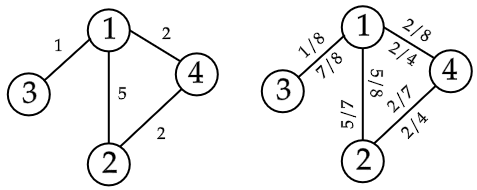
\includegraphics[width=0.9\textwidth]{fig-1.png}
    \end{center}
  \end{marginfigure}

  \begin{ex}{Simple Random Walk on a Graph}{label}
    For a simple random walk on a non-weighted graph, 
    \[w(i,j) = 1 \quad \forall i,j \in V(G) \quad \text{ and } \quad w(v) = \text{deg}(v)\]
    If $|E(G)|$ is the number of edges in the graph, this gives,
    \[\pi_{v}=\frac{\operatorname{deg}(v)}{\sum_{z} \operatorname{deg}(z)}=\frac{\operatorname{deg}(v)}{2 |E(G)|}\]
  \end{ex}

  \subsection{Regular Chains}
    \begin{defn}[Regularity]
    A transition matrix $\boldsymbol{P}$ is \textbf{regular} if and only if there exists $n \in \mathbb{N}$ so that every entry of $\boldsymbol{P}^n$ is positive.
  \end{defn}

  \begin{thm}
    If the matrix $\boldsymbol{P}^n$ is regular, then $\boldsymbol{P}^m$ is regular ($m > n$).
  \end{thm}

  \begin{proof}
    Linear combinations of positive numbers are positive, so the result follows by the definition of matrix multiplication,
    \[\boldsymbol{P}_{i j}^{n+1}=\sum_{\ell \in S} \boldsymbol{P}_{i \ell}^{n} \cdot \boldsymbol{P}_{\ell j}>0\]
    \noindent since $\boldsymbol{P}_{i \ell}^{n}>0$ and at least one $\boldsymbol{P}_{\ell j}$ is positive\footnote{Otherwise $\boldsymbol{P}^n$ has a zero column.}.
  \end{proof}

  \begin{marginfigure}
    The two-state Markov chain with,
    \[\boldsymbol{P}=\left(\begin{array}{cc}1-p & p \\ q & 1-q\end{array}\right)\]
    \noindent can be expressed as,
    \begin{center}
    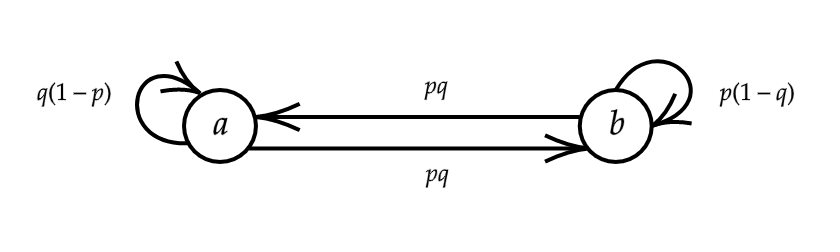
\includegraphics[width=\textwidth]{fig-13.png}
    \end{center}
    \noindent Therefore, its stationary distribution is,
    \[\pi=\left(\frac{q}{p+q}, \frac{p}{p+q}\right)\]
  \end{marginfigure}


  \begin{thm}
    A stochastic matrix $\boldsymbol{P}$ has an eigenvalue $\lambda^* = 1$. All other eigenvalues $\lambda$ of $\boldsymbol{P}$ satisfy $|\lambda| \leq 1$, with strict inequality if $P$ is regular.
    \label{perronlemma}
  \end{thm}

  \begin{marginfigure}
    \textbf{Example of Regularity:}

    \noindent The following matrix is regular,
    \[\boldsymbol{P}=\left(\begin{array}{ccc}0 & 1 / 2 & 1 / 2 \\ 1 & 0 & 0 \\ 1 / 2 & 1 / 2 & 0\end{array}\right)\]
    \noindent because $\boldsymbol{P}^4$ is positive,
    \[\boldsymbol{P}^{4}=\left(\begin{array}{ccc}9 / 16 & 5 / 16 & 1 / 8 \\ 1 / 4 & 3 / 8 & 3 / 8 \\ 1 / 2 & 5 / 16 & 3 / 16\end{array}\right)\]
    \begin{center}
    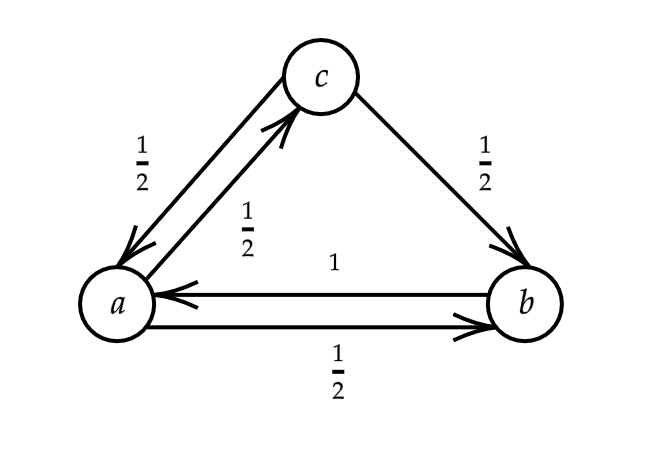
\includegraphics[width=\textwidth]{fig-12.png}
    \end{center}
  \end{marginfigure}

  \begin{proof}
    Let $\boldsymbol{P}$ be a $k \times k$ stochstic matrix. The rows of $\boldsymbol{P}$ sum to 1 by definition, so $\boldsymbol{P} \cdot \Vec{1} = \Vec{1}$ and $\lambda^* = 1$ is a right eigenvalue of $\boldsymbol{P}$. Suppose that $\Vec{z}$ is the eigenvector corresponding to any other eigenvalue $\lambda$ of $\boldsymbol{P}$. Let $|z_m| = \max_{1 \leq i \leq k} |z_i|$ be the component of $\Vec{z}$ of maximum absolute value. Then,
    \[
    |\lambda| \cdot |z_m| = |\lambda z_m| = |(\boldsymbol{P} \cdot \Vec{z})_m| = |\sum_{i = 1}^{k} \boldsymbol{P}_{mi}z_i| \leq |z_m| \sum_{i = 1}^{k} \boldsymbol{P}_{mi} = |z_m|
    \]
    \noindent and consequently $|\lambda| \leq 1$.

    Assume that $\boldsymbol{P}$ is regular. Then $\boldsymbol{P}^n > 0$ for some $n > 0$. $\boldsymbol{P}$ is a stochastic matrix, and it was shown above that $\boldsymbol{P}$ has an eigenvalue $\lambda^* = 1$. Moreover, all other eigenvalues $\lambda$ of $\boldsymbol{P}$ satisfy $|\lambda| \leq 1$. We want to show that the inequality is strict. If $\lambda$ is an eigenvalue of $\boldsymbol{P}$, then $\lambda^n$ is an eigenvalue of $\boldsymbol{P}^n$. Let $\Vec{x}$ be its corresponding eigenvalue, with $|x_m| = \max_{1 \leq i \leq k} |x_i|$. Then,
    \[
    |\lambda|^n \cdot |x_m| = |(\boldsymbol{P}^n \cdot \Vec{z})_m| = |\sum_{i = 1}^{k} \boldsymbol{P}^n_{mi}x_i| \leq |x_m| \sum_{i = 1}^{k} \boldsymbol{P}^n_{mi} = |x_m|
    \]
    \noindent Since the entries of $\boldsymbol{P}^n$ are positive, the last inequality only holds if $|x_1| = \cdots = |x_k|$. Similarly, the first inequality only holds if $x_1 = \cdots = x_m$. But the constant vector whose components are the same is an eigenvector associated with the eigenvalue 1. Hence, if $\lambda \neq 1$, one of the inequalities must be strict. Thus, $|\lambda|^n < 1$.
  \end{proof}

  \begin{thm}
   Every finite state time-homogeneous Markov chain $(X_n)_{n \geq 0}$ has a stationary distribution $\Vec{\pi}$. Moreover, the stationary distribution(s) of $(X_n)$ are in bijective correspondance with the left 1-eigenvectors of $\boldsymbol{P}$\footnote{We require that the eigenvectors are non-negative with components that sum to 1.}.
  \end{thm}

  \begin{proof}
    If $\boldsymbol{P}$ is a stochastic matrix, then $\boldsymbol{P}$ has a right eigenvalue $\lambda^* = 1$ (see Theorem \ref{perronlemma}). Since det$(\boldsymbol{P}^T) =$ det$(\boldsymbol{P})$, the left and right eigenvalues of $\boldsymbol{P}$ are equal. Hence, $\boldsymbol{P}$ has at least one left eigenvector $\Vec{\pi}$ for the eigenvalue 1. Normalizing this eigenvector to sum to 1 gives\footnote{The vector with $|\pi|_i = |\pi_i|$ is still an eigenvector with eigenvalue 1.},
    \[\boldsymbol{P} \cdot \Vec{\pi} = 1 \cdot \Vec{\pi} \quad \text{i.e., } \boldsymbol{P} \cdot \Vec{\pi} = \Vec{\pi}\]
    The proof that the stationary distribution(s) of $(X_n)$ are in bijective correspondance with the left 1-eigenvectors of $\boldsymbol{P}$ is similar.
  \end{proof}

  \begin{cor}
    If $(X_n)$ has a unique stationary distribution, then the distribution is a left eigenvector of $\boldsymbol{P}$ corresponding to $\lambda^* = 1$.
  \end{cor}

  \begin{thm}[Perron-Frobenius]
    Let $\boldsymbol{M}$ be a $k \times k$ positive matrix. Then,
    \begin{itemize}
      \item There exists $\lambda^* \in \mathbb{R}^+$ (called the Perron-Frobenius eigenvalue) which is an eigenvalue of $M$. $|\lambda| < \lambda^*$ for all other eigenvalues $\lambda$ of $\boldsymbol{M}$.
      \item The eigenspace of eigenvectors associated with $\lambda^*$ is one-dimensional
    \end{itemize}
  \end{thm}
  
  \begin{proof}
    The proof of the Perron–Frobenius theorem can be found in many linear algebra textbooks, including Horn and Johnson (1990).
  \end{proof}

  \begin{thm}[Limit Theorem for Finite Regular Chains]
    If $(X_n)_{n \geq 0}$ is a finite state time-homogeneous Markov chain and $\boldsymbol{P}$ is regular, then there is a unique, positive, stationary distribution $\Vec{\pi} > 0$ such that,
    \[ \lim_{n \rightarrow \infty} P^n = \boldsymbol{V}\]
    \noindent where \textbf{V} is a matrix with all rows equal to $\Vec{\pi}.$
  \end{thm}

  \subsection{Classification of States}
  \begin{marginfigure}
    \textbf{Example of Communication Classes:}

    \noindent $G$ has 3 communication classes,
    \begin{center}
    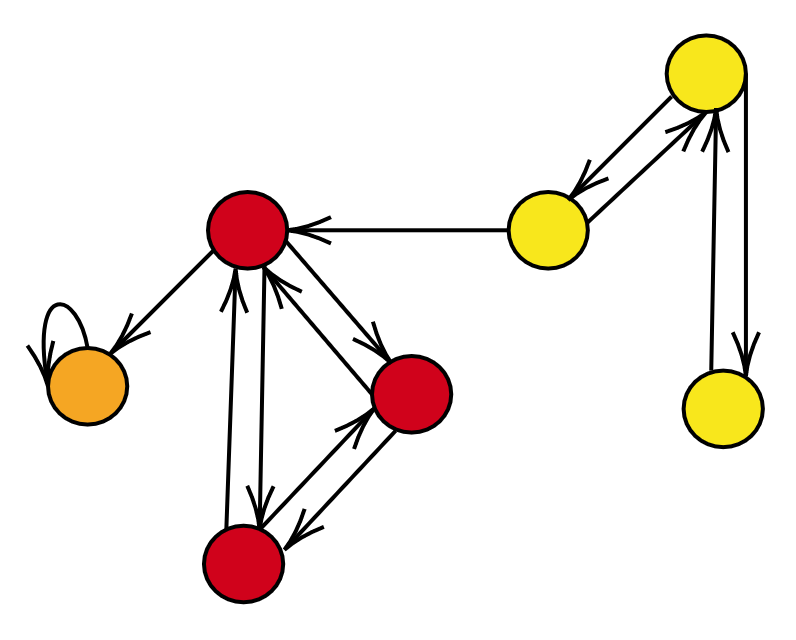
\includegraphics[width=0.6\textwidth]{fig-2.png}
    \end{center}
    
  \end{marginfigure}

  \begin{defn}[Communication]
    Two states $i, j \in S$ of a Markov chain \textbf{communicate}, written $i \leftrightarrow j$, if there exist $m, n \in \mathbb{N}$ such that,
    \[p_m(i,j) > 0 \quad \text{and} \quad p_n(j,i) > 0\]
    \noindent Equivalently, two states communicate if and only if each state has a positive probability of eventually being reached by a chain starting in the other state.
  \end{defn}

  \begin{thm}
    The relation $\leftrightarrow$ is an equivalence relation on the state space.
  \end{thm}

  \begin{proof}
    The relation $\leftrightarrow$ is reflexive, symmetric, and transitive.
    \begin{itemize}
      \item (Reflexivity) $i \leftrightarrow i$ since $p_0(i,i) = 1 > 0$
      \item (Symmetry) $i \leftrightarrow j \implies j \leftrightarrow i$ by definition
      \item (Transitivity) $i \leftrightarrow j$ and $j \leftrightarrow i \implies i \leftrightarrow k$ since,
      \begin{align*}
        p_{m_1 + m_2}(i,k) &= P(X_{m_1 + m_2} = k \text{ $|$ } X_0 = i) \\
        &\geq P(X_{m_1 + m_2} = k, X_{m_1} = j \text{ $|$ } X_0 = i) \\
        &= P(X_{m_1} = j \text{ $|$ } X_0 = i) \cdot P(X_{m_1 + m_2} = k \text{ $|$ } X_{m_1} = j) \\
        &= p_{m_1}(i,j)p_{m_2}(j,k) \\
        &> 0
      \end{align*}
    \end{itemize}
  \end{proof}

  \begin{defn}[Irreducibility]
      The relation $\leftrightarrow$ partitions the state space into disjoint sets called \textbf{communication classes}. If there is only one communication class, then the chain is called irreducible.
  \end{defn}

  \begin{defn}[Hitting Time]
    Let $(X_n)_{n \geq 0}$ be a Markov chain with state space $S$. The \textbf{hitting time} ("first passage time") of $A \subseteq S$ when $X_0 = x$ is,
    \[\tau_A = \inf \{n \geq 0 \text{ $|$ } X_n \in A\}\]
  \end{defn}

  \begin{defn}[First Return Time]
    Let $(X_n)_{n \geq 0}$ be a Markov chain with state space $S$. The \textbf{first return time} is a variant of hitting time,
    \[\tau^+_x = \inf \{n \geq 1 \text{ $|$ } X_n = i\} \quad \text{ assuming } \quad \text{$X_0 = x$}\]
  \end{defn}

  \begin{defn}[Expected Number of Visits]
    Let $(X_n)_{n \geq 0}$ be a Markov chain with state space $S$. The \textbf{expected number of visits} to $i \in S$ is,
    \[\sum_{n=0}^\infty p_n(i,i) \quad \text{ assuming } \quad \text{$X_0 = i$}\]
  \end{defn}

  \begin{proof}
    Let $N_i$ be the random variable giving the total number of visits to $i \in S$, including the initial visit. We can write,
    \[N_i = \sum_{n=0}^\infty \mathbbm{1}_{\{X_n = i\}}\]
    \noindent where the expectation of $N_i$ when $X_0 = i$ is,
    \[\mathbb{E}[N_i] = \mathbb{E}\bigg[\sum_{n=0}^\infty \mathbbm{1}_{\{X_n = i\}}\bigg] = \sum_{n=0}^\infty P(X_n = i) = \sum_{n=0}^\infty p_n(i,i)\]
  \end{proof}

  \begin{thm}[Limit Theorem for Finite Irreducible Chains]
      If $(X_n)_{n \geq 0}$ is a finite state time-homogeneous Markov chain and $\boldsymbol{P}$ is irreducible, then,
      \[\mu_j = \mathbb{E}[\tau^+_j \mid X_0 = j] < \infty \quad \text{for all $i \in S$}\]
      \noindent and there exists a unique, positive, stationary distribution $\Vec{\pi} > 0$ such that,
      \[\pi_{j}=\frac{1}{\mathbb{E}[\mu_j]}, \text { for all } j \in S\]
      \noindent Furthermore,
      \[\pi_{j}=\lim _{n \rightarrow \infty} \frac{1}{n} \sum_{m=0}^{n-1} \boldsymbol{P}_{i j}^{m} \quad \text { for all } j \in S\]
  \end{thm}

  \subsection{First Step Analysis}
  \begin{defn}[First-Step Analysis]
    \textbf{First-step analysis} is the process of conditioning on the first step of the chain and using the law of total expectation to find the expected return time, $\mathbb{E}[\tau^+_j \text{ $|$ } X_0 = j]$.
  \end{defn}

  \begin{rmk}
    If $(X_n)_{n \geq 0}$ is irreducible, then the expected return time can also be found by taking the reciprocal of the stationary probability $\pi$.
  \end{rmk}

  \begin{ex}{First-Step Analysis}{label}
    Consider the Markov chain with transition matrix,
    \[\boldsymbol{P} = \begin{blockarray}{cccc}
    a & b & c \\
    \begin{block}{(ccc)c}
      0 & 1 & 0 & a \\
      1/2 & 1 & 1/2 & b \\
      1/3 & 1/3 & 1/3 & c \\
    \end{block}
    \end{blockarray}\]

    Define $e_x := \mathbb{E}[\tau_j^+ \mid X_0 = x]$ for $x \in \{a, b, c\}$. Thus, $e_a$ is the desired expected return time, and $e_b$, $e_c$ are the first hitting times to $a$ for the chain started in $b$ and $c$.
    \begin{align*}
      &e_a = 1 + e_b \\
      &e_b = \frac{1}{2} + \frac{1}{2}(1 + e_c) \\
      &e_c = \frac{1}{3} + \frac{1}{3}(1 + e_b) + \frac{1}{3}(1 + e_c)
    \end{align*}
    \noindent Solving these equations gives,
    \[e_{c}=\frac{8}{3} \quad e_{b}=\frac{7}{3} \quad e_{a}=\frac{10}{3}\]
  \end{ex}

  \subsection{Recurrence and Transience}
  \begin{defn}[Recurrent]
    A state $i \in S$ is \textbf{recurrent} if a Markov chain starting at $i$ will return to $i$ infinitely often, with probability 1.
  \end{defn}

  \begin{defn}[Transient]
    A state $i \in S$ is \textbf{transient} if a Markov chain starting at $i$ will return to $i$ only finitely often, with probability 1.
  \end{defn}

  \begin{thm}
    Recurrence and transience are class properties,
    \begin{align*}
      \text{If $i \in S$ is recurrent and $j \leftrightarrow i$} &\implies \text{$j$ is recurrent} \\
      \text{If $i \in S$ is transient and $j \leftrightarrow i$} &\implies \text{$j$ is transient}
    \end{align*}
  \end{thm}

  \begin{proof}
    It suffices to show that if $i \in S$ is transient and $j \leftrightarrow i$, then $j$ is transient. Since $j \leftrightarrow i$, there exist $s,r \geq 0$ such that $p_s(i,j) > 0$ and $p_r(j,i) > 0$. For all $n \in \mathbb{N}$, it holds that,
    \[p_{n+r+s}(i,i) \geq p_{s}(i,j) \cdot p_{n}(j,j) \cdot p_{r}(j,i)\]
    \noindent by Chapman-Kolmogorov. Therefore,
    \begin{align*}
      \sum_{n=1}^{\infty} p_{n}(j,j) &\leq \frac{1}{p_{s}(i,j) \cdot p_{r}(j,i)} \sum_{n=1}^{\infty} p_{n+r+s}(i,i) \text{ expanding the expectation} \\ &\leq \frac{1}{p_{s}(i,j) \cdot p_{r}(j,i)} \sum_{n=1}^{\infty} p_{n}(i,i) \\
      &<\infty \quad \text{since $i$ is transient}
    \end{align*}
    \noindent It follows that $j$ is transient. Hence, if one state of a communication class is transient, all states in that class are transient.

    Conversely, if one state is recurrent, then the others must be recurrent. By contradiction, if the communication class contains a transient state then by what was just proven all the states are transient.
  \end{proof}

  \begin{thm}
    Every state in a finite, irreducible Markov chain is recurrent.
  \end{thm}

  \begin{proof}
    Every pair $i, j \in S$ belongs to the same communication class, and that class has finitely many elements. By definition, there is positive probability of reaching $j$ from $i$ since $i \leftrightarrow j$. If $i$ is visited infinitely often then we get this chance of visiting $j$ infinitely often. If an event has a positive probability of occuring, and we get an infinite number of trials, then it will occur an infinite number of times.
  \end{proof}

  \begin{thm}
    Let $(X_n)_{n \geq 0}$ be an irreducible Markov chain. Then,
    \[\mathbb{E}[N_i]  = \sum_{n=0}^\infty p_n(i,i)
                       = \frac{1}{1 - P(\tau^+_i < \infty)}
                       = \frac{1}{P(\tau^+_i = \infty)}
                       = (I - \boldsymbol{P})_{ii}^{-1}\]
    \noindent Moreover,
    \[\mathbb{E}[N_i] = \begin{cases}
                          \text{finite} & \text{$\iff i$ is transient} \\
                          \text{infinite} & \text{$\iff i$ is recurrent}
                        \end{cases}\]
  \end{thm}

  \begin{marginfigure}
  \textbf{Recall:}

  \noindent Let $\boldsymbol{A}$ be a square matrix with the property that $\boldsymbol{A}^n \rightarrow 0$, as $n \rightarrow \infty$. Then, $\sum_{n=0}^{\infty}A^n = (I - A)^{-1}$. This gives the matrix analog of the sum of a geometric series of real numbers.
  \end{marginfigure}

  \begin{proof}
    Assume that $\mathbb{E}[N_i] < \infty$. Let $R_i$ be the number of returns to a state $i$. Define a sequence $(\tau^{(n)}_i)_{n \geq 0}$ by,
    \[\tau^{(n)}_i = \begin{cases}
      \inf \{n \geq 1 \text{ $|$ } X^*_n = i\} & R_i \geq n\\
      \infty & \text{otherwise}
    \end{cases}\]
    \noindent where $(X^*_n)$ is the process $(X_n)$ started at $\tau^{(n-1)}_i$. $N_i = \sum_{n=1}^{\infty} \mathbbm{1}_{\{X_n = i\}}$ is 1 more than the number of returns $R_i$, so,
    \[N_i = 1 + R_i = 1 + \sum_{n=1}^{\infty} \mathbbm{1}_{\{\tau^{(n)}_i < \infty\}}\]
    \noindent and $\tau^{(n)}_i = \infty$ if and only if $X_n$ visits $i$ fewer than $n$ times. Now, $P(\tau^{(n)}_i < \infty) = [P(\tau^{(1)}_i = \infty)]^n$ by time homogeneity $(\star)$. Therefore,
    \begin{align*}
      \mathbb{E}[N_i] &= \mathbb{E}\bigg[1 + \sum_{n=1}^{\infty} \mathbbm{1}_{\{\tau^{(n)}_i < \infty\}}\bigg] \\
      &= \mathbb{E}\bigg[\sum_{n=0}^{\infty} \mathbbm{1}_{\{\tau^{(n)}_i < \infty\}}\bigg] \\
      &= \sum_{n=0}^{\infty} \mathbb{E}\bigg[\mathbbm{1}_{\{\tau^{(n)}_i < \infty\}}\bigg] \quad \text{ by Linearity of Expectation} \\
      &= \sum_{n=0}^{\infty} P(\tau^{(n)}_i < \infty) \\
      &= \sum_{n=0}^{\infty} P(\tau^{(1)}_i < \infty) \\
      &= \sum_{n=0}^{\infty} [P(\tau^{(1)}_i < \infty)]^n \quad (\star) \\
      &= \frac{1}{1 - P(\tau^+_i < \infty)} \quad \text{by definition of a geometric series}
    \end{align*}
    \noindent Thus, $\mathbb{E}[N_i] = \frac{1}{1 - P(\tau^+_i < \infty)}  = \begin{cases}
                          \text{finite} & \text{$\iff i$ is transient} \\
                          \text{infinite} & \text{$\iff i$ is recurrent}
                        \end{cases}$
  \end{proof}

  \begin{marginfigure}
    \textbf{Stirling's Formula} states that as $n \rightarrow \infty$,
    \[n ! \sim \sqrt{2 \pi n}\left(\frac{n}{e}\right)^{n}\]
  \end{marginfigure}

  \begin{ex}{Simple Symmetric Random Walk on $\mathbb{Z}$}{label}
  The \textbf{simple symmetric random walk on $\mathbb{Z}$} is recurrent,
  \begin{center}
  
\includegraphics[width=\textwidth]{fig-14.png}
  \end{center}
  \begin{align*}
    \mathbb{E}[N_i] &= \sum_{n \geq 0} p_n(0,0) \\
                    &= \sum_{n \geq 0} p_{2n}(0,0) \\
                    &= \sum_{n \geq 0} \binom{2n}{n} \cdot \frac{1}{2^{2n}} \\
                    &\geq \sum_{n \geq 1} \frac{1}{\sqrt{4n}} \text{ by Stirling's Formula} \\
                    &= \infty
  \end{align*}
  \end{ex}

  \begin{defn}[Canonical Decomposition]
    The \textbf{canonical decomposition} of the state space $S$ of a finite Markov chain is a separation of $S$,
    \[S = T \cup R_1 \cup \cdots \cup R_m\]
    \noindent where $R_1, \cdots, R_m$ are the communication classes of recurrent states and $T$ is the set of all transient states. $\boldsymbol{P}$ has the block matrix form,
    \[
    \boldsymbol{P} = \begin{blockarray}{cccccc}
    T & R_1 & R_2 & \cdots & R_m \\
    \begin{block}{(ccccc)c}
      * & * & * & \cdots & * & T \\
      0 & \boldsymbol{P}_1 & 0 & \cdots & 0 & R_1 \\
      0 & 0 & \boldsymbol{P}_2 & \cdots & 0 & R_2 \\
      \vdots & \vdots & \vdots & \ddots &  \vdots & \vdots \\
      0 & 0 & 0 & 0 & \boldsymbol{P}_m & R_m \\
    \end{block}
    \end{blockarray}
     \]
     \noindent where each square stochastic matrix $\boldsymbol{P}_i$ corresponds to a closed recurrent communication class which is irreducible with a restricted state space\footnote{A communication class is \textbf{closed} if it consists of all recurrent states.}.
    \end{defn}

    \begin{rmk}
      The block matrix form facilitates taking matrix powers,
          \[
          \lim_{n \rightarrow \infty} \boldsymbol{P}^n = \begin{blockarray}{cccccc}
          T & R_1 & R_2 & \cdots & R_m \\
          \begin{block}{(ccccc)c}
            * & * & * & \cdots & * & T \\
            0 & \lim_{n \rightarrow \infty} \boldsymbol{P}^n_1 & 0 & \cdots & 0 & R_1 \\
            0 & 0 & \lim_{n \rightarrow \infty} \boldsymbol{P}^n_2 & \cdots & 0 & R_2 \\
            \vdots & \vdots & \vdots & \ddots &  \vdots & \vdots \\
            0 & 0 & 0 & 0 & \lim_{n \rightarrow \infty} \boldsymbol{P}^n_m & R_m \\
          \end{block}
          \end{blockarray}
           \]
    \end{rmk}
    
    \begin{cor}
    For every recurrent class $R_i$, there is a stationary distribution $\Vec{\pi}$ so that $\pi_i>0$ if and only if $i\in R_i$.
    \end{cor}

    \begin{cor}
    The dimension of the eigenspace of $\boldsymbol{P}$ for the eigenvalue 1 is the number of recurrent classes in the Markov chain.
    \end{cor}

  \subsection{Periodicity}
  \begin{defn}[Period]
    The \textbf{period} of a state $i$, $d = d(i)$ is,
    \[\text{gcd}(J_i) \text{ where } J_i = \{n \geq 0 \text{ $|$ } p_n(i,i) > 0\}\]
    \noindent If $d(i) = 1$, state $i$ is called aperiodic.
  \end{defn}

  \begin{thm}
    The states of a communication class all have the same period.
  \end{thm}

  \begin{proof}
    Suppose that there exist states $i, j$ such that $i \leftrightarrow j$ and $d(i) \neq d(j)$. Since $i$ and $j$ communicate, there exist $r, s \in \mathbb{N}$ such that,
    \[p_m(i,j) > 0 \quad \text{and} \quad p_n(j,i) > 0\]
    \noindent Then $m + n$ is a possible return time for $i$,
    \[p_{m + n}(i,i) = \sum_{k \in S} p_m(i,k) \cdot p_n(k,i) \geq p_m(i,j) \cdot p_n(j,i) > 0\]
    \noindent and $d(i)$ is a divisor of $m + n$. Assume that $p_r(j,j) > 0$ for some integer $r$. Then $p_{r + m + n}(i,i) \geq p_m(i,j) \cdot p_r(j,j) \cdot p_n(j,i) > 0$ and $d(i)$ is a divisor of $r + m + n$. Since $d(i)$ divides both $m + n$ and $r + m + n$, it must also divide $r$. Thus, $d(i)$ is a common divisor of the set $\{r > 0 \mid p_r(j,j) > 0\}$. Since $d(j)$ is the largest such divisor, $d(i) \leq d(j)$. A symmetric argument gives that $d(j) \leq d(i)$.
  \end{proof}

  \begin{ex}{Periodicity}{label}
    A random walk on the $n$-cycle has no limiting distribution when $n$ is even. The graph is regular, and the unique stationary distribution is uniform. However, the chain alternates between even and odd states, and its position after $n$ states depends on the parity of the initial state. 
  \end{ex}

  \begin{defn}[Periodic Chain]
    A Markov chain is \textbf{periodic} if it is irreducible and all states have period greater than 1.
  \end{defn}

  \begin{defn}[Aperiodic Chain]
    A Markov chain is \textbf{aperiodic} if it is irreducible and all states have period equal to 1.
  \end{defn}

  \begin{marginfigure}
    \textbf{Note on Periodicity:}

    \noindent Any state $i$ satisfying that $\boldsymbol{P}_{ii} > 0$ is necessarily aperiodic. Thus, a suficient condition for an irreducible Markov chain to be aperiodic is that $\boldsymbol{P}_{ii} > 0$ for some $i$, i.e., at least one diagonal entry of the transition matrix is non-zero.
  \end{marginfigure}

    \begin{thm}
    \textbf{P} is irreducible and aperiodic if and only if $\boldsymbol{P}$ is regular.
  \end{thm}

  \begin{proof}
    Suppose that $\boldsymbol{P}$ is irreducible and aperiodic. Consider any states $i,j$. Since $\boldsymbol{P}$ is irreducible, there exists $m(i,j)$ so that $p_{m(i,j)}(i,j) > 0$. Since $\boldsymbol{P}$ is aperiodic, there exists $M(i)$ so that for all $n \geq M(i)$, $p_n(i,i) > 0$. Taken together, this means that for $n \geq M(i)$,
    \[p_{n+m(i,j)}(i,j) \geq p_n(i,i)p_{m(i,j)}(i,j) > 0\]
    \noindent Now, $p_n(i,j) > 0$ for all $n \geq \max \{M(i) + m(i,j) \text{ $|$ } (i,j) \in S \times S\}$.

    Suppose that $\boldsymbol{P}$ is regular. By definition, there exists an $M > 0$ such that for all $n \geq M$, $\boldsymbol{P}^n$ has all entries strictly positive. This means that $p_n(i,j) > 0$ for all states $i,j$, and consequently that $\boldsymbol{P}$ is irreducible. If $\boldsymbol{P}^n$ has strictly positive entries, so too does $\boldsymbol{P}^{n+1}$. Thus, $P(X_n = i \text{ $|$ } X_0 = i) > 0$ and $P(X_{n+1} = i \text{ $|$ } X_0 = i) > 0$. Since $gcd(n, n+1) = 1$, $\boldsymbol{P}$ is aperiodic. 
  \end{proof}

  
  \begin{thm}[Limit Theorem for Aperiodic Irreducible Chains]
    If $(X_n)_{n \geq 0}$ is a finite state, time-homogeneous, aperiodic, irreducible Markov chain and $\boldsymbol{P}$ is its transition matrix, then there is a unique, positive, stationary distribution $\Vec{\pi} > 0$ such that,
    \[ \lim_{n \rightarrow \infty} P^n = \boldsymbol{V}\]
    \noindent where \textbf{V} is a matrix with all rows equal to $\Vec{\pi}.$
  \end{thm}

  \subsection{Absorbing Chains}
  \begin{defn}[Absorption]
    A state $i \in S$ is called \textbf{absorbing} if,
    \[p(i, i) = 1\]
    An absorbing chain has at least one absorbing state\footnote{Intuitively, this is a state $i$ that the chain never leaves once it first visits $i$.}.
  \end{defn}

  \begin{defn}[Absorption Probability]
    Let $(X_n)_{n \geq 0}$ be a Markov chain with all states transient or absorbing. The \textbf{absorption probability} is the probability that the chain is absorbed in state $j$ from transient state $i$. 
  \end{defn}

  \begin{defn}[Absorption Time]
    Let $(X_n)_{n \geq 0}$ be a Markov chain with all states transient or absorbing. The \textbf{absorption time} is the expected number of steps from transient state $i$ to absorption in some absorbing state.
  \end{defn}

  \begin{marginfigure}
    \textbf{Note on Absorption Time:}

    \noindent The problem of computing hitting time reduces to the problem of computing time to absorption because a state can be modified to be absorbing.
  \end{marginfigure}

  \begin{thm}
    Let $(X_n)_{n \geq 0}$ be finite-state and irreducible with transition matrix \textbf{P}. To find the expected hitting time, $\mathbb{E}[\tau_i]$,
    \begin{itemize}
      \item Consider a new chain in which $i$ is an absorbing state
      \item Define $\boldsymbol{\tilde{P}}$ by deleting the $i$th row and setting $\boldsymbol{\tilde{P}}_{ii} = 1$
      \item Define $\boldsymbol{Q}$ by deleting the $i$th row and $i$-h column of $\boldsymbol{P}$
    \end{itemize}
  \noindent Assume that the chain starts in state $a$. The first time that $\boldsymbol{P}$ hits $i$ is,
  \[
    \begin{cases}
      \sum_{b \neq i} (\boldsymbol{I} - \boldsymbol{\tilde{P}})^{-1}_{a,b} & \text{if $i \neq a$} \\
      1 + \sum_{j \neq i} \boldsymbol{P}_{ij} \cdot \sum_{b \neq i} (\boldsymbol{I} - \boldsymbol{\tilde{P}})^{-1}_{j,b} & \text{if $i = a$}
    \end{cases}
  \] 
  \end{thm}

  \begin{proof}
    We need to find,
    \begin{align*}
      \mathbb{E}[\tau_a] &= \mathbb{E}[\inf \{n \geq 0 \text{ $|$ } X_n \in A\}] \\
      &= \sum_{n=1}^\infty n \cdot P(\tau_a = n) \\
      &= \sum_{n=1}^\infty P(\tau_a \geq n)
    \end{align*}
    \noindent For an absorbing state $a$,
    \[P(\tau_a \geq n) = P(X_{n-1} \neq a) \quad \text{ ($n \geq 1$)}\]
    \noindent Considering every probable path that does not go through $a$,
    \begin{align*}
      \mathbb{E}[\tau_a] &= \sum_{i = 1}^k \sum_{n = 1}^{\infty} \sum_{b \neq a} \pi_i \cdot \boldsymbol{\tilde{P}}_{i, b}^{n-1} \\
      &= \sum_{i = 1}^k \sum_{b \neq 1} \pi_i (\boldsymbol{I} - \boldsymbol{\tilde{P}})^{-1}_{i,b}
    \end{align*}
  \end{proof}

  \subsection{Positive and Null Recurrence}
  \begin{defn}[Positive Recurrent]
    A recurrent state $j$ is \textbf{positive recurrent} if the expected return time $\mathbb{E}[\tau^+_j \text{ $|$ } X_0 = j]$ is finite\footnote{Positive recurrence is the infinite analog of finite recurrent chains.}.
  \end{defn}

  \begin{thm}[Limit Theorem for Irreducible, Positive Recurrent Chains]
    Let $(X_n)_{n \geq 0}$ be an infinite, irreducible, and positive recurrent Markov chain. There exists a unique, positive, stationary distribution $\pi$, which is the limiting distribution of the chain\footnote{For infinite irreducible chains that are null recurrent, no stationary distribution exists.}. That is,
     \[\pi_j = \lim_{n \rightarrow \infty}\boldsymbol{P}_{ij}^n \quad \text{ for all $i,j$}\]
    \noindent Moreover,
    \[\pi_j = \frac{1}{\mathbb{E}[\tau^+_j]} \quad \text{ for all $j$}\] 
  \end{thm}

  \begin{defn}[Null Recurrent]
    A recurrent state $j$ is \textbf{null recurrent} if the expected return time $\mathbb{E}[\tau^+_j \text{ $|$ } X_0 = j]$ is infinite\footnote{Null recurrent chains do not have stationary distributions.}.
  \end{defn}

  \begin{thm}
    Positive and null recurrence are class properties\footnote{In particular, all states in a recurrent communication class are either positive or null recurrent.}.
  \end{thm}

  \begin{proof}
    Assume that $i$ is a positive recurrent state. Let $j$ be another state in the same communication class as $i$. Since $i \leftrightarrow j$, there exist $s,r \geq 0$ such that $p_r(j,i) > 0$ and $p_s(i,j) > 0$. Thus,
    \begin{align*}
    \frac{1}{\mu_{j}} &=\lim _{n \rightarrow \infty} \frac{1}{n} \sum_{m=0}^{n-1} p_m(j,i) \\
    & \geq \lim _{n \rightarrow \infty} \frac{1}{n} \sum_{m=r+s}^{n-1} p_r(j,i) \cdot p_{m-r-s}(i,i) \cdot p_{s}(i,j) \\
    &=\lim _{n \rightarrow \infty}\left(\frac{n-r-s}{n}\right) p_r(j,i) \left(\frac{1}{n-r-s} \sum_{m=r+s}^{n-1} p_{m-r-s}(i,i)\right) P_{s}(i,j) \\
    &=p_r(j,i)\left(\frac{1}{\mu_{i}}\right) p_s(i,j)>0 .
    \end{align*}
    \noindent Hence, $\mu_j < \infty$ and $j$ is positive recurrent.
  \end{proof}

  \begin{defn}[Ergodic]
    A Markov chain is called \textbf{ergodic} if it is irreducible, aperiodic, and all states have finite expected return times\footnote{Every finite chain is ergodic, and the condition that all states have finite expected return times is equivalent to all states being positive recurrent.}.
  \end{defn}

  \begin{thm}[Limit Theorem for Ergodic Chains]
    Let $(X_n)_{n \geq 0}$ be an ergodic Markov chain. There exists a unique, positive, stationary distribution $\pi$, which is the limiting distribution of the chain. That is,
    \[\pi_j = \lim_{n \rightarrow \infty}\boldsymbol{P}_{ij}^n \quad \text{ for all $i,j$}\]
    \noindent Moreover,
    \[\pi_j = \frac{1}{\mathbb{E}[\tau^+_j]} \quad \text{ for all $j$}\] 
  \end{thm}

  \subsection{Reversibility}
  \begin{defn}[Detailed Balance Equations]
  \[\pi_i\boldsymbol{P}_{ij} = \pi_j\boldsymbol{P}_{ji} \quad \text{ for all $i,j \in S$}\]
  \noindent More generally, we can write,
  \[P(X_0 = i_0, X_1 = i_1, \cdots, X_n = i_n) = P(X_0 = i_n, X_1 = i_{n-1}, X_n = i_0)\]
  \end{defn}

  \begin{thm}
    Let $(X_n)_{n \geq 0}$ be a Markov chain with transition matrix \textbf{P}. If $\Vec{\pi}$ satisfies the detailed balance equations, then $\Vec{\pi}$ is stationary\footnote{Checking detailed balance is often the simplest way to verify that a particular distribution is stationary.} for \textbf{P}. 
  \end{thm}

  \begin{proof}
    $\sum_{i \in S} \pi_i\boldsymbol{P}_{ij} = \sum_{i \in S}\pi_j\boldsymbol{P}_{ji} = \pi_j$ since \textbf{P} is stochastic.
  \end{proof}

  \begin{defn}
    An irreducible Markov chain $(X_n)_{n \geq 0}$ with transition matrix \textbf{P} and stationary distribution $\Vec{\pi}$ is \textbf{time reversible} if it satisfies the detailed balance equations. The time reversal of $(X_n)$ is the chain with,
    \[\hat{\boldsymbol{P}}_{ij} := \frac{\pi_j\boldsymbol{P}_{ij}}{\pi_i}\]
    \noindent as its transition matrix.
  \end{defn}

  \begin{rmk}
    If a chain with transition matrix $\boldsymbol{P}$ is reversible, then $\hat{\boldsymbol{P}} = \boldsymbol{P}$.
  \end{rmk}

  \begin{proof}
    By the detailed balance equations,
    \[\hat{\boldsymbol{P}}_{ij} = \frac{\pi_j\boldsymbol{P}_{ij}}{\pi_i} = \frac{\pi_j\boldsymbol{P}_{ji}}{\pi_i}\]
    \noindent so $\boldsymbol{P}_{ji} = \boldsymbol{P}_{ij}$.
  \end{proof}

  \begin{ex}{Reversibility}{label}
    A simple random walk on a graph is time reversible.
    \begin{align*}
      \pi_{i} \boldsymbol{P}_{i j} &=\left(\frac{\operatorname{deg}(i)}{2 |E(G)|}\right)\left(\frac{1}{\operatorname{deg}(i)}\right) \quad \text{for neighbors $i,j$}\\
      &=\frac{1}{2 |E(G)|}\\
      &=\left(\frac{\operatorname{deg}(j)}{2 |E(G)|}\right)\left(\frac{1}{\operatorname{deg}(j)}\right)\\
      &=\pi_{j} \boldsymbol{P}_{j i}
    \end{align*}
  \end{ex}

  \section{Markov Chain Monte Carlo}
  \subsection{Markov Chain Coupling}
  \begin{defn}[Total Variation Distance]
    The \textbf{total variation distance} between two distributions $\mu$ and $\nu$ on a state space $S$ is defined by\footnote{This definition is explicitly probabilistic: the distance between $\mu$ and $\nu$ is the maximum difference between the probabilities assigned to a single event by the two distributions.},
    \[\|\mu - \nu\|_{TV} = \sup_{A \subseteq S}\|\mu(A) - \nu(A)\|\] 
  \end{defn}

  \begin{ex}{Coupling Distance}{label}
    Suppose, for illustration, that the total variation distance,
    \[\|\pi_7 - \pi\|_{TV} = 0.17\]
    This tells us that the probability of any event, for example, the probability of winning any specified card game using a deck shuffled 7 times, differs by at most 0.17 from the probability of the same event using a perfectly shuffled deck.
  \end{ex}

  \begin{marginfigure}
    A \textbf{coupling of two probability distributions} $\mu$ and $\nu$ is a pair of random variables $(X, Y )$ defined on a single probability space such that the marginal distribution of $X$ is $\mu$ and the marginal distribution of $Y$ is $\nu$.
    \vphantom{.}
    \noindent That is, a coupling $(X, Y)$ satisfies,
    \[P(X = x) = \mu(x) \text{ and } P(Y = y) = \nu(y)\]
  \end{marginfigure}

  \begin{defn}[Coupling of Markov Chains]
    A \textbf{coupling of Markov chains} is a process $(X_n, Y_n)_{n \geq 0}$ with the property that both $(X_n), (Y_n)$ are Markov chains with transition matrix \textbf{P}, although the chains may have different starting distributions.
  \end{defn}

  \begin{defn}[Coupling Time]
    The \textbf{coupling time} of a process $(X_n, Y_n)_{n \geq 0}$ is defined to be the first time $T$ in which $X_n$ equals $Y_n$,
    \[T = \inf\{n \text{ $|$ } X_n = Y_n\}\]
  \end{defn}

  \begin{lem}
    Consider a coupling $(X_n, Y_n)_{n \geq 0}$ of Markov chains $(X_n), (Y_n)$.
    \[\|\Vec{\pi_0} \cdot \boldsymbol{P}^n - \Vec{\pi}\|_{TV} \leq P(T > n) \text{ for all $n > 0$}\]
    \noindent where $\Vec{\pi}$ is the stationary distribution of $(Y_n)$.
  \end{lem}

  \begin{marginfigure}
    The coupling inequality reduces the problem of showing that,
    \[\|\Vec{\pi_0} \cdot \boldsymbol{P}^n - \Vec{\pi}\| \rightarrow 0\]
    \noindent to that of showing,
    \[P(T > n) \rightarrow 0 \iff P(T < \infty) = 1\]
  \end{marginfigure}

  \begin{proof}
    Define the process $(Y_n^*)$ by,
    \[
    Y_n^* = \begin{cases}
      Y_n & \text{if $n < T$} \\
      X_n & \text{if $n \geq T$}
    \end{cases}
    \]
    \noindent $(Y_n^*)$ is a Markov chain with the same probability transition matrix \textbf{P} as $(X_n)$. This is because $Y_n$ and $X_n$ share \textbf{P} and $Z_n$ and $X_n$ share $\Vec{\pi_0}$. Since we also have that $(Y_n^*) \sim \pi$ for all $n$, 
    \begin{align*}
      \Vec{\pi_0} \cdot \boldsymbol{P}^n(A) - \Vec{\pi} &= P(X_n \in A) - P(Y_n^* \in A) \\
                                             &= P(X_n \in A, T \leq n) + P(X_n \in A, T > n) \\
                                             &\text{  } - P(Y_n^* \in A, T \leq n) - P(Y_n^* \in A, T > n)
    \end{align*}
    \noindent However, on the event $\{T \leq n\}$, $Y_n^* = X_n$, so that $P(X_n \in A, T \leq n) = P(Y_n^* \in A, T \leq n)$. Simplifying gives that,
    \[\Vec{\pi_0} \cdot \boldsymbol{P}^n(A) - \Vec{\pi} = P(X_n \in A, T > n) - P(Y_n^* \in A, T > n) < P(T > n)\]
  \end{proof}

  \begin{rmk}[Doeblin Coupling Argument]
    Proving the Markov Convergence Theorem can be done by showing that $P(T < \infty) = 1$.
  \end{rmk}

  \begin{proof}
    The bivariate chain $Z = \{(X_n, Y_n) \text{ $|$ } n \geq 0\}$ is a Markov chain on the state space $S \times S$. Its transition matrix $\boldsymbol{P}^Z$ can be written,
    \[\boldsymbol{P}^Z_{(i_1, i_2), (j_1, j_2)} = \boldsymbol{P}^X_{(i_1, j_1)}\cdot\boldsymbol{P}^Y_{(i_2, y_2)}\]
    \noindent and the stationary distribution is,
    \[\pi^Z(i,j) = \pi_i\pi(y)\]
    \noindent $P(T < \infty) = 1$ occurs if the $Z$ chain hits $\{(j,j) \text{ $|$ } j \in S\} \subseteq S \times S$. Since $Z$ has a stationary distribution, it suffices to show that $Z$ is irreducible\footnote{If an irreducible Markov chain has a stationary distribution, then the chain is recurrent.}. This can be done using a numbertheoretic proof.
  \end{proof}

  \subsection{Metropolis-Hastings Algorithm}
  \begin{defn}[Markov Chain Monte Carlo]
    Given a discrete or continuous probability distribution $\Vec{\pi}$, the goal of \textbf{Markov Chain Monte Carlo} is to simulate a random variable $X \sim \Vec{\pi}$.
  \end{defn}

  \begin{rmk}[Strong Law of Large Numbers for Markov Chains]
    If $(X_n)_{n \geq 0}$ is a finite state, time-homogeneous, aperiodic, irreducible Markov chain and $r$ is a bounded and real-valued function, then\footnote{The chain is not i.i.d, but successive excursions between visits to the same state are independent.},
    \[\lim_{n \rightarrow \infty} \frac{r(X_1)+ \cdots + r(X_n)}{n} = \mathbb{E}[r(X)] \quad \text{ a.s. }\]
    \noindent where $\mathbb{E}[r(X)] = \sum_j r(j) \pi_j$.
  \end{rmk}

  \begin{defn}[Metropolis-Hastings Algorithm]
    Let $\Vec{\pi}$ be a discrete probability distribution. The \textbf{Metropolis-Hastings Algorithm} constructs a reversible Markov chain $(X_n)_{n \geq 0}$ whose stationary distribution is $\Vec{\pi}$,
    \begin{enumerate}
      \item Let \textbf{T}, the proposal chain, be a transition matrix\footnote{It is assumed that the user knows how to sample from \textbf{T}.} for any irreducible Markov chain with the same state space as $\Vec{\pi}$
      \item Assume that at time $n$, the chain is at state $i$
      \item Choose a new state $j$, the proposal state, according to $\boldsymbol{T}_{ij}$
      \item Let $U \sim Unif(0,1)$. If $X_n = i$, define an acceptance function,
      \[
      a(i,j) = \frac{\pi_j\boldsymbol{T}_{ji}}{\pi_i\boldsymbol{T}_{ij}} \quad
      \text{ and let } X_{n+1} := \begin{cases}
        j & \text{if $U \leq a(i,j)$} \\
        i & \text{otherwise}
        \end{cases}
      \]
    \end{enumerate}
  \end{defn}

  \begin{proof}
    The sequence $(X_n)_{n \geq 1}$ constructed by the Metropolis-Hastings Algorithm is a Markov chain, as each $X_{n+1}$ only depends on $X_n$. Let \textbf{P} be its transition matrix. We need to show that $(X_n)$ is reversible with stationary distribution is $\Vec{\pi}$. Given $X_0 = i$, then,
    \begin{align*}
      P(U \leq a(i,j)) &= \begin{cases}
                          a(i,j) & \text{if $a(i,j) \leq 1$} \\
                          1 & \text{otherwise}
                          \end{cases} \\
                       &= \begin{cases}
                          a(i,j) & \text{if $\pi_j\boldsymbol{T}_{ji} \leq \pi_i\boldsymbol{T}_{ij}$} \\
                          1 & \text{otherwise}
                          \end{cases} \\
    \end{align*}
    \noindent and for $i \neq j$, 
    \begin{align*}
      \boldsymbol{P}_{ij} &= \begin{cases}
                      \boldsymbol{T}_{ij} \cdot a(i,j) & \text{ if $\pi_j\boldsymbol{T}_{ji} \leq \pi_i\boldsymbol{T}_{ij}$} \\
                      \boldsymbol{T}_{ij} & \text{otherwise}
                      \end{cases}
    \end{align*}
    \noindent The diagonal entries of \textbf{P} are determined by the fact that the rows of \textbf{P} sum to 1. There are two cases,
    \begin{itemize}
      \item If $\pi_j\boldsymbol{T}_{ji} \leq \pi_i\boldsymbol{T}_{ij}$,
      \[\pi_i\boldsymbol{P}_{ij} = \pi_i\boldsymbol{T}_{ij}a(i,j) = \pi_i\boldsymbol{T}_{ij}\bigg(\frac{\pi_j\boldsymbol{T}_{ij}}{\pi_i\boldsymbol{T}_{ij}}\bigg) = \pi_j\boldsymbol{T}_{ji} = \pi_j\boldsymbol{P}_{ji}\]
      \item If $\pi_j\boldsymbol{T}_{ji} < \pi_i\boldsymbol{T}_{ij}$,
      \[\pi_i\boldsymbol{P}_{ij} = \pi_i\boldsymbol{T}_{ij}a(i,j) = \pi_j\boldsymbol{T}_{ji}\bigg(\frac{\pi_i\boldsymbol{T}_{ij}}{\pi_j\boldsymbol{T}_{ji}}\bigg) = \pi_j\boldsymbol{T}_{ji}a(j,i) = \pi_j\boldsymbol{P}_{ji}\]
    \end{itemize}
    \noindent Hence, the detailed balance equations are satisfied.
  \end{proof}

  \section{Classical Markov Chains}
  \subsection{Electrical Networks}
  We can represent Markov chains as electrical networks, which we typically denote by undirected weighted graphs $G = (V, E)$.

  \begin{defn}[Electrical Network]
    A \textbf{network} is a pair $(G, c)$, where $G = (V, E)$ is a countable graph and $c: E \rightarrow (0, \infty)$ is a function assigning a positive \textbf{conductance} to each edge such that,
    \[C_x := \sum_{y \sim x} C_{xy} < \infty \quad \forall x \in V\]
    \noindent and $(X_n)_{n \geq 0}$ is a random walk with transition matrix,
    \[\boldsymbol{P}_{xy} := \frac{C_{xy}}{C_x}\]
  \end{defn}

  \begin{defn}[Resistance]
    The \textbf{resistance} $R_{xy}$ of an edge $e = (x,y)$ is,
    \[R_{xy} = \frac{1}{C_{xy}}\]
    \noindent That is, it is the reciprocal of its conductance.
  \end{defn}

  \begin{defn}[Effective Conductance]
    The \textbf{effective conductance} between two disjoint, non-empty finite sets of vertices $A$ and $B$ is defined,
    \[c_{A,B}^{\texttt{eff}} := \sum_{v \in A} c_a \cdot P(\tau_{v} < \tau^+_b)\]
    \noindent where $\tau_v$ is the first hitting time and $\tau_a^+$ is the first return time\footnote{Recall that we write $\tau_z$ and $\tau^+_a$ for the first time that the random walk visits $z$ and the first positive time that the random walk visits $a$ respectively.}. When $A = \{a\}$ and $B = \{b\}$, the effective conductance is,
    \[C_{A,B}^{\texttt{eff}} := \sum_{v \in A} C_a \cdot P(\tau_{v} < \tau^+_b \text{ $|$ } X_0 = a)\]
    \noindent When $A$ and $B$ are not disjoint, we define $C_{A,B}^{\texttt{eff}} = \infty$.
  \end{defn}

  \begin{defn}[Effective Resistance]
    The \textbf{effective resistance} between two disjoint, non-empty finite sets of vertices $A$ and $B$ is defined,
    \[R_{A,B}^{\texttt{eff}} = \frac{1}{C_{A,B}^{\texttt{eff}}}\]
  \end{defn}

  \begin{rmk}[Series Additivity]
    Vertices connected in series can be replaced by one vertex whose resistance is the sum of the resistances.
  \end{rmk}

  \begin{rmk}[Parallel Additivity]
    Vertices connected in parallel can be replaced by one vertex whose conductance is the sum of the conductances.
  \end{rmk}

  \begin{rmk}
    Given a network $G$ and two disjoint, finite, non-empty sets of vertices $A$ and $B$, we can form a network $G^{\prime}$ by contracting ("shorting") each of the sets $A$ and $B$ into single vertices $[A]$ and $[B]$. Then,
    \[c_{A,B}^{\texttt{eff}}(G) = c_{[A],[B]}^{\texttt{eff}}(G^{\prime})\]
  \end{rmk}

  \begin{marginfigure}
    \textbf{Shorting} two vertices adds infinite conductance between them (or, merges them while preserving edges). Thus, shorting two sets of nodes can only decrease the effective resistence of the network between two nodes.
    \begin{center}
    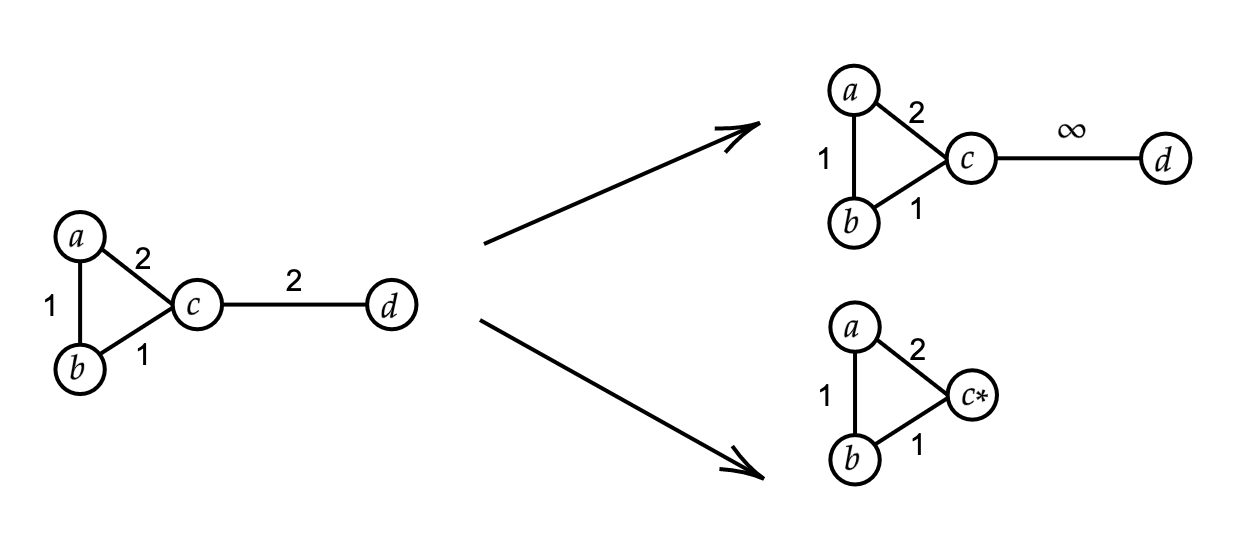
\includegraphics[width=\textwidth]{fig-10.png}
    \end{center}

    \noindent \textbf{Cutting} an edge can only increase the effective resistance between the two vertices that it is adjacent to.
  \end{marginfigure}

  \begin{rmk}[Rayleigh's Monotonicity Principle]
    Let $G = (V, E)$ be a finite graph, and let $A$ and $B$ be disjoint, non-empty subsets of $V$. Then, 
    \[c_{A,B}^{\texttt{eff}}(G)\]
    is a \textbf{monotone increasing} function of $c \in (0, \infty)^E$.
  \end{rmk}
  
  \begin{rmk}
    An irreducible Markov chain $(X_n)$ is recurrent if and only if the conductance to infinity, $\lim_{n \rightarrow \infty} C_{0, [n]}$, is finite,
    \[P(\tau_0 < \infty) = \lim_{n \rightarrow \infty} C_{0, [n]} < \infty\]
  \end{rmk}

  \subsection{P\'{o}lya's Theorem}
  \begin{thm}[P\'{o}lya's Theorem]
    The $d$-dimensional hybercubic lattice $\mathbb{Z}^d$ is recurrent if $d \leq 2$ and transient if $d \leq 3$.
  \end{thm}

  \begin{cor}
    A simple random walk on any subgraph of $\mathbb{Z}^2$ is recurrent\footnote{Adding a finite number of edges to a transient graph preserves transience.}.
  \end{cor}

  \subsection{P\'{o}lya's Urn}
  \begin{defn}[P\'{o}lya Urn Model]
    \textbf{P\'{o}lya's Urn} is the process,
    \begin{itemize}
      \item An urn contains two balls, one black and one white
      \item Proceed by choosing a ball at random from those already in the urn
      \item Return the chosen ball to the urn and add another ball of the same color
    \end{itemize}
    \noindent The sequence of ordered pairs listing the numbers of black and white balls is a Markov chain. A configuration $(a, b)$ with $a$ black balls and $b$ white balls evolves according to,
    \[(a,b) \rightarrow \begin{cases}
      (a+1, b) & \text{ with probability $\frac{a}{a+b}$} \\
      (b, b+1) & \text{ with probability $\frac{b}{a+b}$} \\
    \end{cases}\]
  \end{defn}

  \begin{marginfigure}
  \begin{center}
  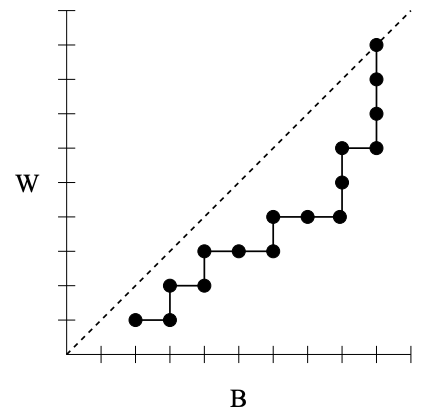
\includegraphics[width=\textwidth]{fig-11.png}
  \caption{The urn process as a trajectory on a two-dimensional lattice, where bullets indicate intermediate stages.}
  \end{center}
  \end{marginfigure}

  \begin{ex}{P\'{o}lya's Urn}{label}
    We want to find the likelihood that the system reaches,
    \[(B, W) = (m,n) \quad \text{ starting from } \quad (B, W) = (b,w)\]
    \noindent Consider the transition,
    \[(1,1) \rightarrow (3,3)\]
    \noindent where one possible path is,
    \[(1,1) \rightarrow (1,2) \rightarrow (1,3) \rightarrow (2,3) \rightarrow (3,3)\]
    Its likelihood is,
    \[\frac{1}{2} \times \frac{2}{3} \times \frac{1}{4} \times \frac{2}{5}=\frac{(1 \cdot 2) \cdot(1 \cdot 2)}{2 \cdot 3 \cdot 4 \cdot 5}\]
    \noindent there are $\binom{4}{2} = 6$ distinct routes, each with this same probability. In general, for a path  $(b,w) \rightarrow (m,n)$,
    \[\frac{[b(b+1) \cdots(m-1)] \cdot[w(w+1) \cdots(n-1)]}{(b+w)(b+w+1) \cdots(m+n-1)}\]
    \noindent Rewriting this probability using factorials,
    \[\frac{(m-1) !}{(b-1) !} \times \frac{(n-1) !}{(w-1) !} \times \frac{(b+w-1) !}{(m+n-1) !}\]
    \noindent 
    The total number of distinct paths from $(b,w)$ to $(m,n)$ is,
    \[\binom{m+n-b-w}{m-b}\]
    \noindent so the transition probability $P$ that, starting from configuration $(b,w)$, the system reaches $(m,n)$ is:
    \[P=\left(\begin{array}{c}
    m-1 \\
    b-1
    \end{array}\right)\left(\begin{array}{c}
    n-1 \\
    w-1
    \end{array}\right)\left(\begin{array}{c}
    m+n-1 \\
    b+w-1
    \end{array}\right)^{-1}\]
  \noindent In particular, for $(b,w) = (1,1)$,
  \[P = \frac{1}{m+n-1} \quad \text{ or, if $U = m+n$, } \quad P = \frac{1}{U}\]
  \end{ex}

  \section{Branching Processes}
  \subsection{Mean Generation Size}
  \begin{marginfigure}
    \begin{center}
    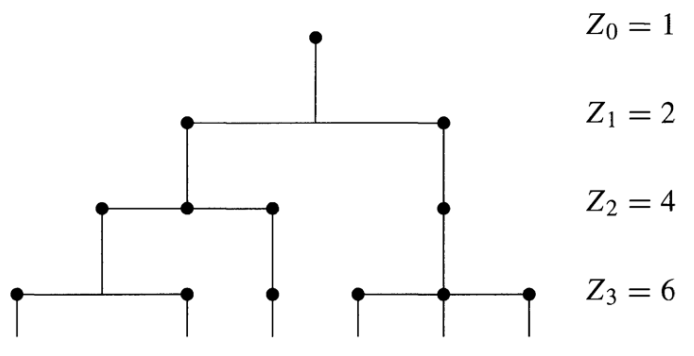
\includegraphics[width=\textwidth]{fig-15.png}
      \caption{Family tree.}
      \end{center}
  \end{marginfigure}

  \begin{defn}[Offspring Distribution]
    The \textbf{offspring distribution} $X$ gives the probability $x_k$ that an individual gives birth to $k$ children,
    \[X = (x_1, x_2, \cdots)\]
    \noindent independently of other individuals.
  \end{defn}

  \begin{defn}[Branching Process]
    Let $Z_n$ be a random variable that denotes the size of a population of living species. The Markov chain $(Z_n)_{n \geq 1}$ with values in $\mathbb{N}_0$ is a \textbf{branching process} if,
    \[Z_{n+1} = \sum_{j=1}^{Z_n} X_j\]
    \noindent where $X_j$ denotes the number of children born to the $j$th person in the $n$th generation. $(X_j)_{j \geq 1}$ is an i.i.d sequence with common distribution $X$. Furthermore, $Z_n$ is independent of $(X_j)$.
  \end{defn}

  \begin{defn}[Extinction Time]
    The \textbf{extinction time} $T_0$ of a branching process is the hitting time to zero, that is, $T_0 := \tau_0$.
  \end{defn}

  \begin{defn}[Mean Generation Size]
    The \textbf{mean generation size} $\mu_n$ is the mean size of the $n$th generation, that is, $\mu_k := \mathbb{E}[Z_n]$.
  \end{defn}

  \begin{defn}[Mean Offspring Size]
    The \textbf{mean offspring size} $\mu$ is the mean of the offspring distribution, that is, $\mu_n := \mathbb{E}[X]$.
  \end{defn}

  \begin{thm}
    Let $\mu = \sum_{k = 0}^{\infty} k \cdot x_k$ be the mean of the offspring distribution.
    \[\mathbb{E}[Z_n] = \mu^n\]
  \end{thm}

  \begin{proof}
    By the Total Law of Expectation,
    \begin{align*}
      \mathbb{E}[Z_{n}] &=\sum_{k=0}^{\infty} \mathbb{E}[Z_{n} \mid Z_{n-1}=k] \cdot P\left(Z_{n-1}=k\right) \\
      &=\sum_{k=0}^{\infty} \mathbb{E}\bigg[\sum_{i=1}^{Z_{n-1}} X_{i} \text{ }\bigg|\text{ } Z_{n-1}=k\bigg] \cdot P\left(Z_{n-1}=k\right) \\
      &= \sum_{k=0}^{\infty} \mathbb{E}\bigg[\sum_{i=1}^{k} X_{i} \mid Z_{n-1}=k\bigg] \cdot P\left(Z_{n-1}=k\right) \\
      &=\sum_{k=0}^{\infty} \mathbb{E}\bigg[\sum_{i=1}^{k} X_{i}\bigg] \cdot P\left(Z_{n-1}=k\right) \text{ since } X_i \text{ and } Z_{n-1} \text{ independent} \\
      &= \sum_{k=0}^{\infty} \mu \cdot k P\left(Z_{n-1}=k\right) \\
      &= \mu \cdot \mathbb{E}[Z_{n-1}]
    \end{align*}
    \noindent Iterating the recurrence $\text { for } n \geq 0$ gives that,
    \[\mathbb{E}[Z_{n}]=\mu \mathbb{E}[Z_{n-1}]=\mu^{2} \mathbb{E}[Z_{n-2}]=\cdots=\mu^{n} \mathbb{E}[Z_{0}]=\mu^{n}\]
    \noindent since $Z_0 = 1$
  \end{proof}

\begin{thm}
  If $\mu < 1$, then $P(T_0 > n) \leq \mathbb{E}[Z_{0}]=\mu^{n}$. In particular, the branching process goes extinct with probability 1, $(T_0 < \infty) = 1$.
\end{thm}

\begin{proof}
  By Markov's Inequality,
  \[P(T_0 > n) = P(Z_n \geq 1) \leq \mathbb{E}[Z_n] = \mu^{n}\mathbb{E}[Z_{0}]\]
\end{proof}

\begin{defn}[Criticality]
  A branching process is \textbf{subcritical} if $\mu < 1$, \textbf{critical} if $\mu = 1$, and \textbf{supercritical} if $\mu > 1$. Moreover,
  \[\lim _{n \rightarrow \infty} \mathbb{E}[Z_{n}]=\lim _{n \rightarrow \infty} \mu^{n}= \begin{cases}0, & \text { if } \mu<1 \\ 1, & \text { if } \mu=1 \\ \infty, & \text { if } \mu>1\end{cases}\]
\end{defn}

\begin{marginfigure}
  \textbf{Note on Criticality:}

  \noindent For a subcritical process, mean generation size declines exponentially to zero. For a supercritical process, it exhibits exponential growth.
\end{marginfigure}

\subsection{Generating Functions} 
\begin{defn}[Generating Function]
  Let $X$ be a discrete random variables with values in $\mathbb{N}_0$. The \textbf{probability generating function} of $X$ is,
  \begin{align*}
  G(s) &=\mathbb{E}[s^{X}]=\sum_{k=0}^{\infty} s^{k} \cdot P(X=k) =\sum_{k=0}^{\infty} s^{k} \cdot \pi_k \\
  &=P(X=0)+s P(X=1)+s^{2} P(X=2)+\cdots
  \end{align*}
  \noindent where $\Vec{\pi} = (\pi_k)_{k \geq 0}$ is the law of $X$.
  \end{defn}

  \begin{ex}{Generating Functions}{label}
    Let $X \sim \text{Unif}(\{0,1,2\})$. Then,
    \[G(s)=\frac{1}{3}+s\left(\frac{1}{3}\right)+s^{2}\left(\frac{1}{3}\right)=\frac{1}{3}\left(1+s+s^{2}\right)\]

    Let $X \sim \text{Geom}(p)$. For $|s| < 1$,
    \[G(s)=\sum_{k=1}^{\infty} s^{k} p(1-p)^{k-1}=s p \sum_{k=1}^{\infty}(s(1-p))^{k-1}=\frac{s p}{1-s(1-p)}\]

    Let $X \sim \text{Po}(\mu)$. For $\mu > 0$,
    \[G(s) = \sum_{k=0}^{\infty} \frac{e^{-\mu} \mu^{k}}{k !} \cdot s^{k} = e^{-\mu} \cdot \sum_{k=0}^{\infty} \frac{(\mu s)^{k}}{k !}=e^{-\mu} e^{\mu s} = e^{\mu(s-1)}\]
  \end{ex}

  \begin{marginfigure}
  \textbf{Properties of Generating Functions:}

    \begin{enumerate}
      \item If $X$ and $Y$ satisfy,
            \[G_X(s) = G_Y(s) \quad \forall s\]
            \noindent then $X \overset{law}{=} Y$.
      \item If $X$ and $Y$ are independent, then,
    \[G_{X+Y}(s) = G_X(s) \cdot G_Y(s)\]
    \end{enumerate}
  \end{marginfigure}

\begin{rmk}
  The series $G(s)$ converges absolutely for $|s| \leq 1$.
\end{rmk}

\begin{proof}
  Let $\Vec{\pi}$ be the law of $X$. Then,
  \[|G(s)| = \bigg|\sum_{k=0}^{\infty} s^k \cdot \pi_k \bigg| \leq \sum_{k=0}^{\infty} |s|^k \cdot \pi_k \leq 1\]
  \noindent so $G(s)$ exists and is well-defined for $|s| \leq 1$.
\end{proof}

\begin{thm}
  Let $(X_n)$ be an i.i.d sequence of random variables. Define $Z := \sum_{i = 1}^n X_n$. The probability generating function of $Z$ is $[G_X(s)]^n$.
\end{thm}

\begin{proof}
  Expanding the definition,
  \begin{align*}
    G_Z(s) &= \mathbb{E}[s^Z] \\
           &= \mathbb{E}[s^{\sum_{i = 1}^n X_n}] \\
           &= \mathbb{E}\bigg[\prod_{k=1}^{n} s^{X_{k}}\bigg] \\
           &= \prod_{k=1}^{n} \mathbb{E}[s^{X_{k}}] \text{ by independence} \\
           &= G_{X_{1}}(s) \cdots G_{X_{n}}(s) 
  \end{align*}
  \noindent If $X_n$ is i.i.d., then,
  \[G_{Z}(s)=G_{X_{1}}(s) \cdots G_{X_{n}}(s)=\left[G_{X}(s)\right]^{n}\]
  \noindent where $X$ has the same distribution as $X_i$.
\end{proof}

\begin{thm}
  Probabilities for $X$ can be obtained from the generating function by successive differentiation.  If $G^{(j)}$ is the $j$th derivative of $G$,
  \[G^{(j)}(s)=\sum_{k=j}^{\infty} k(k-1) \cdots(k-j+1) s^{k-j} P(X=j)\]
\end{thm}

\begin{proof}
  Observe that,
  $$
  \begin{aligned}
  G(0) &=P(X=0) \\
  G^{\prime}(0) &=\left.\sum_{k=1}^{\infty} k s^{k-1} P(X=k)\right|_{s=0}=P(X=1) \\
  G^{\prime \prime}(0) &=\left.\sum_{k=2}^{\infty} k(k-1) s^{k-2} P(X=k)\right|_{s=0}=2 P(X=2)
  \end{aligned}
  $$
  and so on. In general,
  $$
  G^{(j)}(0)=\left.\sum_{k=j}^{\infty} k(k-1) \cdots(k-j+1) s^{k-j} P(X=j)\right|_{s=0}=j ! P(X=j)
  $$
  and thus
  $$
  P(X=j)=\frac{G^{(j)}(0)}{j !}, \quad \text { for } j=0,1, \ldots
  $$
\end{proof}

\begin{thm}
  The generating function of the $n$th generation size $Z_n$ is the $n$-fold composition of the offspring distribution generating function,
  \[G_{n}(s)= \mathbb{E}[s^{Z_n}] = \underbrace{G \circ G \circ \cdots \circ G}_{n \text{ times}}(\mathbb{E}[s^{Z_{0}}])\]
\end{thm}

\begin{proof}
  The generating function of the $n$th generation size $Z_n$ is,
  \[G_{n}(s)=\mathbb{E}[s^{Z_{n}}]=\mathbb{E}\bigg[s^{\Sigma_{k=1}^{Z_{n-1}} X_{k}}\bigg]=\mathbb{E}\bigg[\mathbb{E}\bigg[s^{\sum_{k=1}^{Z_{n-1}} X_{k}} \mid Z_{n-1}\bigg]\bigg]\]
  \noindent where the last inequality is by the Total Law of Expectation.
  \begin{align*}
    \mathbb{E}\bigg[s^{\sum_{k=1}^{Z_{n-1}} X_{k}} \mid Z_{n-1} = z\bigg]
    &= \mathbb{E}\bigg[s^{\sum_{k=1}^z X_{k}} \mid Z_{n-1} = z\bigg] \text{ by conditioning} \\
    &= \mathbb{E}\bigg[s^{\sum_{k=1}^z X_{k}}\bigg] \text{ by independence}\\
    &= \mathbb{E}\bigg[\prod_{k=1}^z s^{X_{k}}\bigg] \\
    &= \prod_{k=1}^z \mathbb{E}[s^{X_{k}}] \text{ by independence} \\
    &= [G(s)]^z \text{ for all $z$}
  \end{align*}
  \noindent $G(s)$ is the generating function of the offspring distribution,
  \[G(s) = \sum_{k=0}^{\infty} s^{k} \pi_k\]
  \noindent so this gives that,
  \[\mathbb{E}[s^{\sum_{k=1}^{Z_{n-1}}X_{k}} \mid Z_{n-1}]=[G(s)]^{Z_{n-1}}\]
  \noindent Taking expectations,
  \[G_{n}(s)=\mathbb{E}[G(s)^{Z_{n-1}}]=G_{n-1}(G(s))\]
  \noindent The result follows by induction on $n$.
\end{proof}

\begin{cor}
  The extinction probability of a branching process is,
  \[P(T_0 < \infty) = \lim_{k \rightarrow \infty} \text{ } \lim_{s \rightarrow 0} \text{ } \underbrace{G \circ G \circ \cdots \circ G}_{k \text{ times}}(\mathbb{E}[s^{Z_{0}}])\]
\end{cor}

\begin{proof}
  The generating function for the $n$th generation size $Z_n$ is,
  \[G_{n}(s)=\sum_{k=0}^{\infty} s^{k} P\left(Z_{n}=k\right)\]
  Since $P(T_0 \leq k) = P(Z_k = 0)$,
  \[P(Z_k = 0) = \lim_{s \rightarrow 0} \mathbb{E}[s^{Z_k}] = \lim_{s \rightarrow 0} G_k(s) = \lim_{s \rightarrow 0} \underbrace{G \circ G \circ \cdots \circ G}_{k \text{ times}}(\mathbb{E}[s^{Z_{0}}])\]
  Now, $P(T_0 < \infty) = P(\bigcup_{k=1}^{\infty} \{T_0 \leq k\}) = P(\bigcup_{k=1}^{\infty} \{Z_k = 0\})$. Therefore,
  \begin{align*}
    P(T_0 < \infty) &= P(\bigcup_{k=1}^{\infty} \{Z_k = 0\}) \\
                    &= \lim_{k \rightarrow \infty} P(\{Z_k = 0\}) \text{ since $\{Z_{k} = 0\} \subseteq \{Z_{k+1} = 0\}$}\\
                    &= \lim_{k \rightarrow \infty} \text{ } \lim_{s \rightarrow 0} \text{ } \underbrace{G \circ G \circ \cdots \circ G}_{k \text{ times}}(\mathbb{E}[s^{Z_{0}}])
  \end{align*}
  \noindent by the continuity of measure over increasing unions.
\end{proof}

\begin{thm}
  The probability generating function $G(s)$ of a discrete random variable $X$ is convex and non-decreasing on $[0,1]$ with $G(1) = 1$.
\end{thm}

\begin{proof}
    We have that,
    \begin{align*}
      &1. \quad \text{$G(1) = 1$ since,}\\
      &\quad\quad \mathbb{E}[1^X] = \sum_{k=0}^{\infty} P(X = k) = 1 \\
      &2. \quad \text{$G(s)$ is strictly increasing since,}\\
      &\quad\quad G^{\prime}(s) = \sum_{k=1}^{\infty} ks^{k-1}\pi_k > 0 \quad \text{($s > 0$ and $\pi_k \neq 0$ for all $k \geq 1$)}\\
      &3. \quad \text{$G(s)$ is strictly convex since,}\\
      &\quad\quad G^{\prime\prime}(s) = \sum_{k=2}^{\infty} k(k-1)s^{k-2}\pi_k > 0 \quad \text{($s > 0$ and $\pi_k \neq 0$ for all $k \geq 2$)}
    \end{align*}
\end{proof}

\begin{thm}
  $G^{\prime}(1)$ can be used to find the mean of $X$.
\end{thm}

\begin{proof}
  $G^{\prime}(1) = \sum_{k=1}^{\infty} k \cdot \pi_k = \sum_{k=1}^{\infty} k \cdot P(X = k) = \mathbb{E}[X]$.
\end{proof}

\begin{thm}
  Let $G(s)$ be the probability generating function of a discrete random variable $X$. The smallest positive root of the equation $G(s) = s$ is the probability of eventual extinction, that is, $P(T_0 < \infty)$.
\end{thm}

\begin{proof}
  The extinction probability $P(T_0 < \infty)$ of a branching process is a root of the equation $s = G(s)$. To see this, 
  \begin{align*}
    P(T_0 \leq k) &= P(Z_k = 0) \\
                  &= G_k(0) \\
                  &= G(G_{k-1}(0)) \\
                  &= G(P(Z_{k-1}=0)) \\
                  &= G(P(T_0 \leq k - 1))
  \end{align*}
  \noindent Taking the limits on both sides and using the continuity of $G$,
  \[P(T_0 < \infty) = G(P(T_0 < \infty))\]

  \noindent Let $x$ be a positive solution of $s = G(s)$. We need to show that,
  \[P(T_0 < \infty) = \lim_{k \rightarrow \infty} P(Z_k = 0) \leq x\]

  \noindent The proof is by induction on $k$. Since $G(s)$ is increasing on $(0,1]$ and $x > 0$, $P(Z_1 = 0) = G_1(0) = G(0) \leq G(x) = x$. Assume that $P(Z_k = 0) \leq x$ for $k < n$. Then, $P\left(Z_{n}=0\right)=G_{n}(0)=G\left(G_{n-1}(0)\right)=G\left(P(T_0 \leq k - 1)\right) \leq G(x)=x$. Taking limits as $n \rightarrow \infty$ gives,
  \[P(T_0 < \infty) \leq x\]
\end{proof}

\begin{thm}
  Let $G(s)$ be the probability generating function of a discrete random variable $X$. Exactly one of the following holds,
  \begin{enumerate}
    \item $G(s) = s$ for infinitely many $s \in [0,1]$ and,
    \[\lim_{k \rightarrow \infty} \underbrace{G \circ G \circ \cdots \circ G}_{k \text{ times}}(s) = s \quad \forall s \in [0,1]\]
    \item $G(s) = s$ for two points $s_1, s_2 \in [0,1]$ and,
    \[\lim_{k \rightarrow \infty} \underbrace{G \circ G \circ \cdots \circ G}_{k \text{ times}}(s) = s_2 \quad \forall s \in [0,1] \text{ and } s_2 \neq 1\]
    \item $G(s) = s$ for a unique point $s \in [0,1]$ and,
    \[\lim_{k \rightarrow \infty} \underbrace{G \circ G \circ \cdots \circ G}_{k \text{ times}}(s) = 1 \quad \forall s \in [0,1]\]
  \end{enumerate}
\end{thm}

\begin{proof}
  If $\pi_k = \delta_{1k}$ for all $k \geq 0$, then $G(s) = s$ for all $s \in [0,1]$ and $\mu = 1$. This implies that $G(s)$ has infinitely many fixed points in the interval $[0,1]$. Assume that $\pi_k \neq \delta_{1k}$. Since $G$ is convex, the two curves $y = G(s)$ and $y = s$ can intersect at either one or two points. The derivative of $G(s)$ at $s = 1$ distinguishes these two cases.
    \begin{center}
    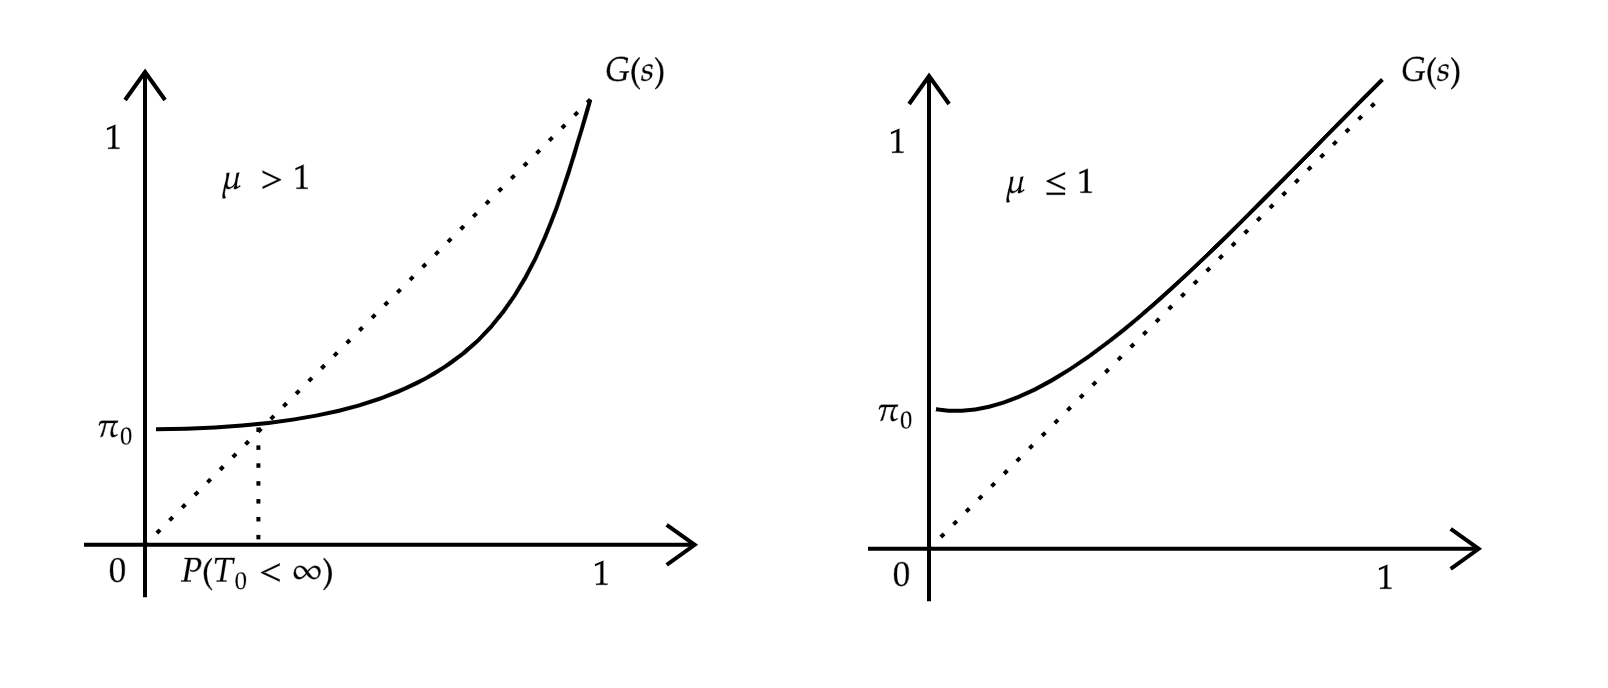
\includegraphics[width=\textwidth]{fig-17.png}
    \end{center}
  \begin{enumerate}
    \item If $\mu \leq 1$, then $G^{\prime}(1) \leq 1$. Since $G^{\prime}$ is strictly increasing in $s$, $G^{\prime}(s)<G^{\prime}(1)=1$ for $0 < s < 1$. Let $h(s) = s - G(s)$. Then $h^{\prime}(s) = 1 -G^{\prime}(s) > 0$ for $0 < s < 1$. But $h$ is increasing and $h(1) = 0$, so $h(s) < 0$ and $s < G(s)$ for $0 < s < 1$. Then, $y = G(s)$ lies above $y = s$ for $0 < s < 1$, and $s = 1$ is the only point of intersection. Thus, $P(T_0 < \infty) = 1$.
    \item If $\mu > 1$, then $G^{\prime}(1) > 1$, then $h(0) = 0 - G(0) = -\pi_0 = -P(X = 0) < 0$ since $P(X = 0) = 0$ contradicts convexity. Also, $h^{\prime}(1) = 1 - G^{\prime}(1) = 1 - \mu < 0$. Thus, $h(s)$ is decreasing at $s = 1$. Since $h(1) = 0$, there exists $0 < t < 1$, such that $h(t) > 0$. It follows that there exists a fixed point $s_2 = G(s_2)$ satisfying $0 < s_2 < 1$. 
  \end{enumerate}
\end{proof}

\begin{ex}{Computing Extinction Probabilities}{label}
  Consider a branching process with,
  \[Z_0 = 1 \quad \text{ and } \quad \Vec{\pi} = \begin{pmatrix} 1/3 & 1/3 & 1/3\end{pmatrix}\]

  where $\Vec{\pi}$ is the offspring distribution. The curves,
  \[y = s \quad \text{ and } \quad y = G(s) = \frac{1}{3}(1 + s + s^2)\]
  \noindent intersect at \text{$s = 1$}. Therefore, \text{$\mu \leq 1$}, and the extinction probability is $P(T_0 < \infty) = 1$. We can also compute $\mu$ explicitly,
  \[\mu=\left.\frac{1}{3}(0+1 \cdot s + 2 \cdot s)\right|_{s=1}=1\]
\end{ex}

\begin{ex}{Computing Extinction Probabilities}{label}
  Consider a branching process with,
    \[Z_0 = 1 \quad \text{ and } \quad \Vec{\pi} \sim \text{Po}(\mu)\]
  where $\Vec{\pi}$ is the offspring distribution. Recall that,
  \[G(s) = e^{\mu(s - 1)}\]
  Solving \text{$s = e^{\mu(s - 1)}$} numerically by iteration,

  \vphantom{.}

  \resizebox{\textwidth}{!}{
    \begin{tabular}{cccccc}
    $G_1(0)$   & $G_2(0)$   & $G_3(0)$   & $G_4(0)$   & $G_10(0)$  & $G_{15}(0)$  \\
    $0.135335$ & $0.177403$ & $0.192975$ & $0.199079$ & $0.203169$ & $0.203187$
    \end{tabular}}
\end{ex}

\begin{marginfigure}
  \begin{center}
      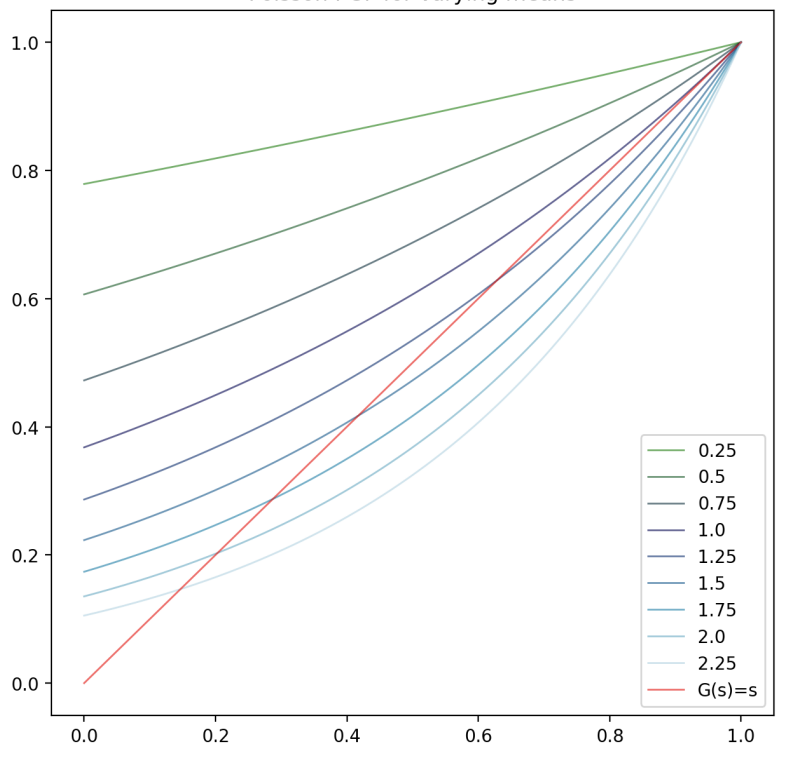
\includegraphics[width=0.9\textwidth]{fig-16.png}
      \caption{A Poisson probability generating function with various means $\mu$.}
    \end{center}
\end{marginfigure}

\section{Poisson Processes}
\subsection{Definition 1}
\begin{defn}[Counting Function]
  A \textbf{counting process} $(N_t)_{t \geq 0}$ is a collection of random variables with values in $\mathbb{N}_0$ such that,
  \[N_t \geq N_s \quad \forall t \geq s \geq 0\]
  \noindent and $\lim_{t \rightarrow s^+} N_t = N_s$ for all $s \in \mathbb{R}$ (right-continuity\footnote{If $0 \leq s < t$, then $N_t - N_s$ is the number of events in the interval $(s, t]$}).
\end{defn}

  \begin{marginfigure}
    \begin{center}
      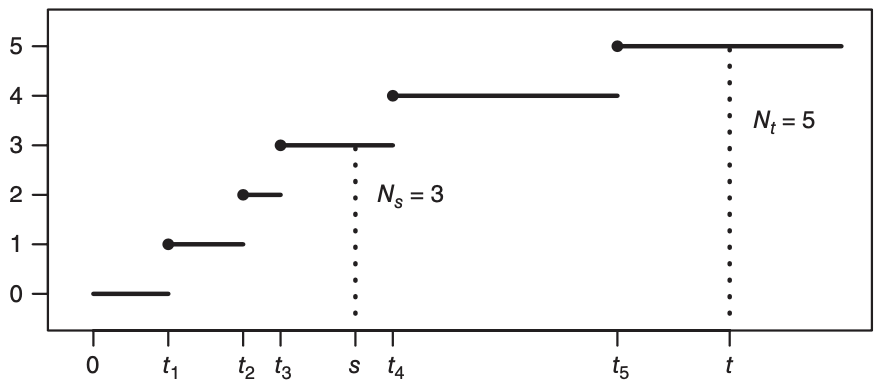
\includegraphics[width=0.9\textwidth]{fig-18.png}
      \caption{Counting process.}
    \end{center}
  \end{marginfigure}

There are three equivalent definitions of a Poisson process, each of which gives special insights into the stochastic model. 

\begin{defn}[Poisson Process -- 1a]
  A \textbf{Poisson process} with parameter $\lambda \geq 0$ is a counting process $(N_t)_{t \geq 0}$ satisfying,
  \begin{enumerate}
    \item $N_0 = 0$
    \item $N_t - N_s \sim \text{Po}(\lambda \cdot (t-s))$ for all $t > s > 0$
    \item $N_t - N_s$ is independent of $N_r$ for all $t > s> 0$ and $0 \leq r \leq s$
  \end{enumerate}
  \noindent where $N_t - N_s$ is the number of events that have occured in $(s, t]$.
\end{defn}

\begin{marginfigure}
  The parameter $\lambda$ is called the \textbf{rate} because $\mathbb{E}[N_t] = t \cdot \lambda$,
  \[\mathbb{E}[N_t] = \mathbb{E}[N_t - N_0] = \lambda \cdot t\]
\end{marginfigure}

\begin{ex}{Poisson Process}{label}
  Jana sends Ioan 10 text messages per hour after 10am. We want to find the probability that Ioan has exactly 18 texts by noon and 70 texts at 5pm. This problem can be modelled by a Poisson process with rate 10, where the desired probability is,
  \[P(N_2 = 18, N_7 = 70)\]
  By definition,
  \[\left\{N_{2}=18, N_{7}=70\right\}=\left\{N_{2}=18, N_{7}-N_{2}=52\right\}\]
  Since $[0,2]$ and $(2, 7]$ are disjoint,
  \begin{align*}
  P\left(N_{2}=18, N_{7}=70\right) &=P\left(N_{2}=18, N_{7}-N_{2}=52\right) \\
  &=P\left(N_{2}=18\right) \cdot P\left(N_{7}-N_{2}=52\right) \\
  &=P\left(N_{2}=18\right) \cdot P\left(N_{5}=52\right) \\
  &=\left(\frac{e^{-20} \cdot 20^{18}}{18 !}\right) \cdot \left(\frac{e^{-50} \cdot 50^{52}}{52 !}\right) \\
  &=0.0045
  \end{align*}
\end{ex}

\begin{defn}[Poisson Process -- 1b]
  A \textbf{Poisson process} with parameter $\lambda \geq 0$ is a counting process $(N_t)_{t \geq 0}$ with,
  \[N_0 = 0 \quad \text{ and } \quad N_t - N_s \sim \text{Po}(\lambda \cdot (t-s))\]
  \noindent for all $t > s > 0$, conditionally on $N_r$ for $0 \leq r \leq s$.
  \label{maximalistprime}
\end{defn}

\begin{lem}
  $N_t - N_s \sim N_{t - s}$\footnote{Be careful when thinking about this conditionally.}
\end{lem}

\begin{proof}
  $N_{t - s} - N_0 \sim \text{Po}(\lambda \cdot (t - s - 0)) = \text{Po}(\lambda \cdot (t - s))$.
\end{proof}

\begin{thm}
  Let $(N_t)_{t \geq 0}$ be a Poisson process with parameter $\lambda$. Then,
  \[(N_{t+s} - N_s)_{t \geq 0} \sim \text{Po}(\lambda) \quad \text{for $s > 0$}\]
  \noindent and $(N_{t+s} - N_s)_{t \geq 0}$ is a Poisson process.
\end{thm}

\begin{proof}
  We need to show that the translated process is probabilistically equivalent to the original process. It suffices to show that, 
  \[Y_t := N_{t+s} - N_s\]
  \noindent is a Poisson Process (Definition 1b). Clearly, $Y_0 = 0$. Now,
  \begin{align*}
    Y_t - Y_r &= N_{t+s} - N_s - (N_{r+s} - N_s) \\
              &=N_{t+s} - N_{r+s}
  \end{align*}
  \noindent so $Y_t - Y_r \sim \text{Po}(\lambda \cdot (t - r))$ given $(N_q)$ for $0 \leq q \leq r$. Furthermore, $(N_q)$ contains all information in $(Y_q) = (N_{q + s} - N_s)$ for $ 0 \leq q \leq r$,
\end{proof}

\subsection{Definition 2}
\begin{defn}[Interarrival Time]
  The \textbf{interarrival} times $(X_k)_{k \geq 0}$ are the times between consecutive jumps of a counting process.
\end{defn}

\begin{defn}[Arrival Time]
  The \textbf{arrival} times $(S_k)_{k \geq 0}$ are the times,
  \[\lim _{t \rightarrow s^+} N_{t} \neq \lim _{t \rightarrow s^-} N_{t}\]
  \noindent at which $(N_t)_{t \geq 0}$ increases.
\end{defn} 

\begin{marginfigure}
  \textbf{Note on Arrival Time:}

  \noindent $S_{K}-S_{k-1}=X_{k} \quad\left(\text{where } S_{0}=0\right)$

  \begin{center}
    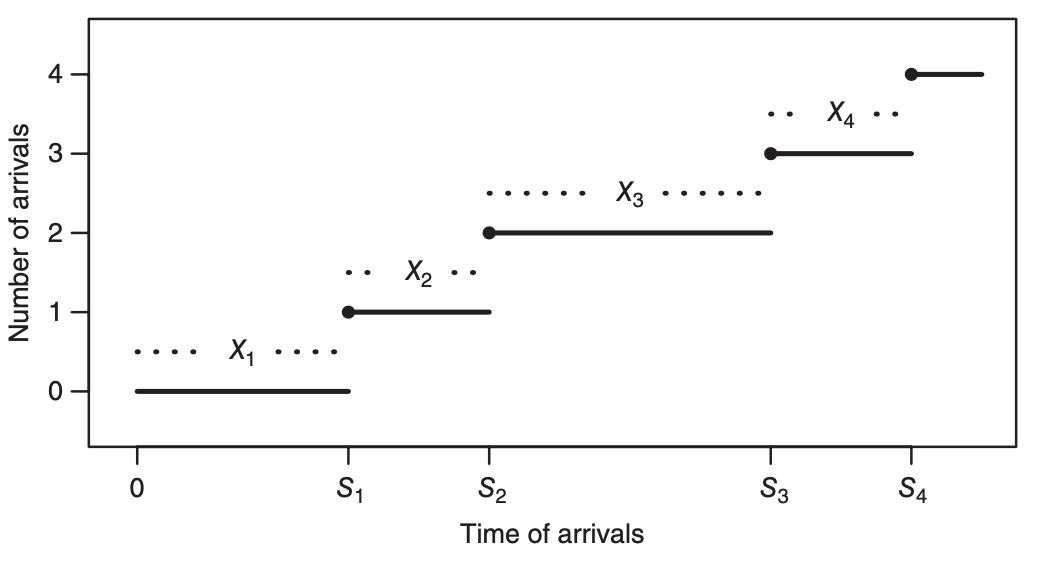
\includegraphics[width=0.9\textwidth]{fig-19.png}
    \caption{Arrival times $S_1, S_2, \cdots$ and interarrival times $X_1, X_2, \cdots$.}
  \end{center}
\end{marginfigure}

\begin{defn}[Poisson Process -- 2]
  Let $(X_n)_{n \geq 0}$ be a sequence of i.i.d exponential random variables with parameter $\lambda$. For $t > 0$, 
  \[N_t = \max \{n \mid X_1 + \cdots X_n \leq t\}\]
  \noindent with $N_0 = 0$. Then, $(N_t)_{t \geq 0}$ is a \textbf{Poisson process} with parameter $\lambda$.
  \[S_n = \sum_{i=1}^n X_i \quad n \in \mathbb{N}\]
  \noindent defines a sequence $(S_n)$ of arrival times of the process, where $S_k$ is the time of the $k$th arrival. The interrarival time between $k-1$ and $k$ is,
  \[X_k = S_k - S_{k-1} \quad k \in \mathbb{N} \quad \text{with $S_0 = 0$}\]
\end{defn}

\begin{marginfigure}
  
  \vphantom{.}

  \noindent \textbf{Note on Exponential Distribution.}

  \vphantom{.}

  \noindent Let $X_i \sim \text{Exp}(\lambda_i)$. Then,

  \noindent $\begin{array}{l}
     \\ P(X \geq t) = e^{-\lambda \cdot t} \\ \\ \hline  \\
     \mathbb{E}[f(X)]  = \int_{0}^{\infty} \lambda e^{-\lambda t} f(t) d t (\star) \\ \\ \hline  \\
     \mathbb{E}[X] = \frac{1}{\lambda} \\ \\ \hline  \\
     G(s) = \mathbb{E}[r^X] = \int_{0}^{\infty} \lambda e^{-\lambda t} r^t d t = \frac{\lambda}{\lambda - \log r}  \\ \\ \hline \\

     P\left(\min \left\{X_{1}, \cdots, X_{n}\right\}>t\right)=e^{-\left(\lambda_{1}+\ldots+\lambda_{n}\right) t}  \\ \\ \hline \\

     P\left(M=X_{i}\right)=\frac{\lambda_{i}}{\lambda_{1}+\cdots+\lambda_{n}} \text{ where } M = \min_i \{X_i\}  \\ \\ \hline \\

     P(X>s+t \mid X>s)=P(X>t) \text { for } s, t>0 \\
    \end{array}$
\end{marginfigure}

\begin{lem}
  If $(N_t)_{t \geq 0}$ is a rate $\lambda \cdot t$ Poisson Process, as in the interarrival definition, then $N_t \sim \text{Po}(\lambda t)$ for all $t \geq 0$.
\end{lem}

\begin{proof}
  Let $(N_t)$ be a rate $\lambda \cdot t$ Poisson Process. Then,
  \[P(N_t = k) = P(\underbrace{\{S_k \leq t\} \cap \{S_{k+1} > t\}}_{:=A}) \quad (k \in \mathbb{N_0})\]
  By the Total Probability Rule,
  \begin{align*}
    P(N_t = k) &= \mathbb{E}[P(A \mid S_k)] \\
               &= \mathbb{E}\big[\mathbbm{1}_{\{S_k \leq t\}} \cdot P(A \mid S_k) + \mathbbm{1}_{\{S_k > t\}} \cdot P(A \mid S_k)\big] \\
               &= \mathbb{E}\big[\mathbbm{1}_{\{S_k \leq t\}} \cdot P(\{S_k \leq t\} \cap \{S_{k+1} > t\} \mid S_k)] \\
               &= \mathbb{E}\big[\mathbbm{1}_{\{S_k \leq t\}} \cdot P(S_{k+1} > t \mid S_k)] \\
               &= \mathbb{E}\big[\mathbbm{1}_{\{S_k \leq t\}} \cdot P(S_{k+1} - S_k > t - S_k \mid S_k)] \\
               &= \mathbb{E}\big[\mathbbm{1}_{\{S_k \leq t\}} \cdot P(X_{k+1} > t - S_k \mid S_k)]
  \end{align*}
  \noindent Applying Property $(\star)$ of the exponential distribution,
  \begin{align*}
    \mathbb{E}\big[\mathbbm{1}_{\{S_k \leq t\}} \cdot P(X_{k+1} > t - S_k \mid S_k)]
    &= \int_0^t e^{-\lambda (t - x)} f(x) d x \\
    &= \int_0^t e^{-\lambda (t - x)} \frac{\lambda^{k} x^{k-1}}{(k-1) !} e^{-\lambda x} d x \\
    &= \frac{\lambda^k \cdot t^k \cdot e^{-\lambda t}}{k !}
  \end{align*}
  \noindent where the density $f(x)$ of $S_k$ can be found using the PGF\footnote{$S_k$ is $\text{Gamma}(k, \lambda)$ distributed, so \[f(x) = \frac{\lambda^{k} x^{k-1}}{(k-1) !} e^{-\lambda x}\]}.
\end{proof}

\begin{defn}[Memoryless]
  A random variable $X$ is \textbf{memoryless} if,
  \[P(X > s + t \mid X > s) = P(X > t)\]
\end{defn}

\begin{lem}
  The exponential distribution is memoryless\footnote{In fact, it is the only continuous distribution that is memoryless.},
\end{lem}

\begin{proof}
  Let $X \sim \text{Exp}(\lambda)$. Then for all $t > s > 0$,
    \[
    P(X > t + s \mid X > s) = \frac{e^{-\lambda(t+s)}}{e^{-\lambda s}}=e^{-\lambda t}
    \]
  \noindent Therefore, $X - s \sim \text{Exp}(\lambda)$ for $X > s$.
\end{proof}

\begin{lem}
  The sum of independent exponentials is exponential.
\end{lem}

\begin{proof}
  Let $X_i \sim \text{Exp}(\lambda_i)$. Then,
  \begin{align*}
  P\left(\min \left(X_{1}, \ldots, X_{n}\right)>t\right)
  &=P\left(X_{1}>t, \ldots, X_{n}>t\right) \\
  &=P\left(X_{1}>t\right) \ldots P\left(X_{n}>t\right) \\
  &=e^{-\lambda_{1} t} \ldots e^{-\lambda_{n} t} \\
  &=e^{-\left(\lambda_{1}+\ldots+\lambda_{n}\right) t}
  \end{align*}
\end{proof}

\begin{marginfigure}
  \textbf{Advantages of Definition 1:}
  \begin{itemize}
    \item Ease of construction and calculation
    \item Explicit law for interarrival times
  \end{itemize}

  \noindent \textbf{Advantages of Definition 2:}
    \begin{itemize}
    \item Independence of increments
    \item Explicit law for statistics of $N_t$
  \end{itemize}
\end{marginfigure}

\begin{ex}{Poisson Process}{label}
  Buses arrive at a bus stop according to a Poisson process with parameter $\lambda = 6$. Suppose that you arrive at 1pm. Then,
  \begin{enumerate}
    \item Probability of waiting at least 15 minutes
    \[P\bigg(\underbrace{S_1}_{= X_1} > \frac{1}{4}\bigg) = \text{Exp}\bigg(-\frac{3}{2}\bigg)\]
    \item Probability that exactly 3 buses arrive in the next hour
    \[P(N_1 = 3) = \frac{6^3}{e^6 \cdot 3!}\]
    \item Expected time to wait for the bus
    \[\mathbb{E}\bigg[\underbrace{S_1}_{= X_1}\bigg] = \frac{1}{6} = 10 \text{ min}\]
    \item 18 buses arrive between 12:50pm and 1:00pm. The expected time to wait for the bus does not depend on the past
    \[\mathbb{E}\bigg[\underbrace{S_1}_{= X_1}\bigg] = \frac{1}{6} = 10 \text{ min}\]
  \end{enumerate}
\end{ex}

\subsection{Definition 3}
\begin{defn}[Poisson Process -- Definition 3]
  A \textbf{Poisson process} with parameter $\lambda$ is a counting process $(N_t)_{t \geq 0}$ satisfying\footnote{There cannot be infinitely many arrivals in a finite interval, and in an infinitesimal interval there may occur at most one event.},
  \begin{enumerate}
    \item $N_0 = 0$
    \item $(N_t)$ has stationary and independent increment
    \item $P(N_h = 0) = 1 - \lambda h + o(h)$
    \item $P(N_h = 1) = \lambda h + o(h)$
    \item $P(N_h > 1) = o(h)$ 
  \end{enumerate}
  \noindent where $f(h) = o(g(h))$ means that,
  \[\lim _{h \rightarrow 0} \frac{f(h)}{g(h)}=0\]
\end{defn}

\section{Applications of Poisson Processes}
\subsection{Thinning and Superposition}
\begin{marginfigure}
  \textbf{Note on Thinning:}

  \noindent Let $Z$ be a Poisson process with parameter $\lambda$. Suppose that $(X_i)_{i \geq 0}$ is a sequence of i.i.d Bernoulli trials with success parameter $p$. If $(X_i)$ is independent of $(N_t)$, then $Y = \sum_{i = 1}^Z X_i \sim \text{Po}(\lambda p)$. To see this, compute the probability generating function of $Y$.
\end{marginfigure}

\begin{defn}[Thinning Poisson Process]
  Let $(N_t)_{t \geq 0}$ be a Poisson process with parameter $\lambda$. Assume that each arrival, independent of other arrivals, is marked as a "Type $k$" ($k \in [n]$) event with probability $p_k$ (where $\sum p_k$ = 1). Let $N_t^{(k)}$ be the number of "Type $k$" events in $[0,t]$. Then,
  \begin{align*}
    &\left(N_t^{(k)}\right)_{t \geq 0} \text{ is a Poisson process with rate $\lambda p_k$} \\
    &\left(N_{t}^{(i)}\right)_{t \geq 0} \text{ and } \left(N_{t}^{(j)}\right)_{t \geq 0} \text{ are independent ($0 \leq i \neq j \leq n$)}
  \end{align*}
  Each process is called a \textbf{thinned Poisson process}.
\end{defn}

\begin{defn}[Superposition Process Poisson]
  Assume that,
  \[\left(N_{t}^{(1)}\right)_{t \geq 0}, \cdots,\left(N_{t}^{(n)}\right)_{t \geq 0}\]
  \noindent are $n$ independent Poisson processes with parameters $\lambda_1, \cdots, \lambda_n$. Let,
  \[N = N_t^{(1)} + \cdots + N_t^{(n)}\]
  \noindent for $t \geq 0$. Then, $(N_t)_{t \geq 0} \sim \text{Po}(t \cdot (\lambda_1 + \cdots + \lambda_n))$.
\end{defn}

\begin{marginfigure}
  \begin{center}
    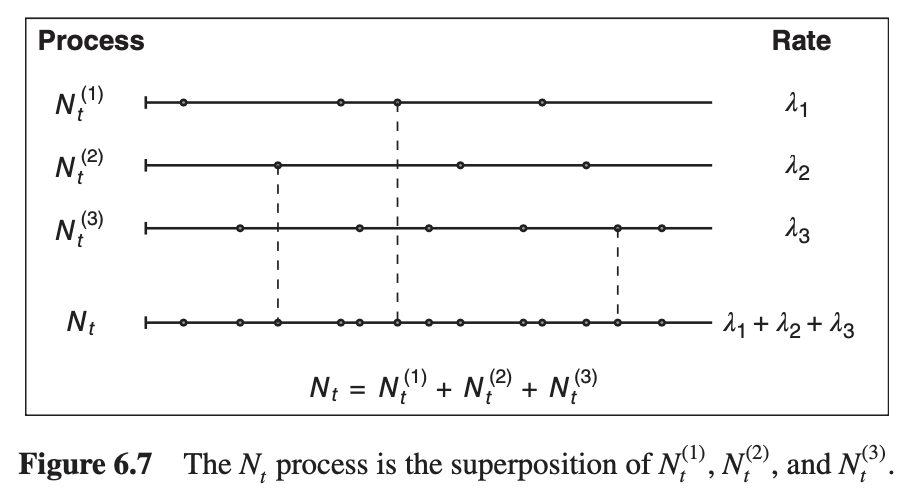
\includegraphics[width=\textwidth]{fig-20.png}
  \end{center}
\end{marginfigure}

\begin{ex}{Birthday Problem}{label}
  The \textbf{Birthday Problem} asks: "If people enter a room one by one, how many people are in the room the first time two people share a birthday, ignoring year and leap days?"

  \vphantom{.}

  This problem can be embedded in a superposition of a Poisson process. People enter a room according to a Poisson process \text{$(N_t)_{t \geq 1}$} with rate \text{$\lambda = 1$}. Each person is independently and uniformly marked with one of 365 birthdays.
  \begin{center}
    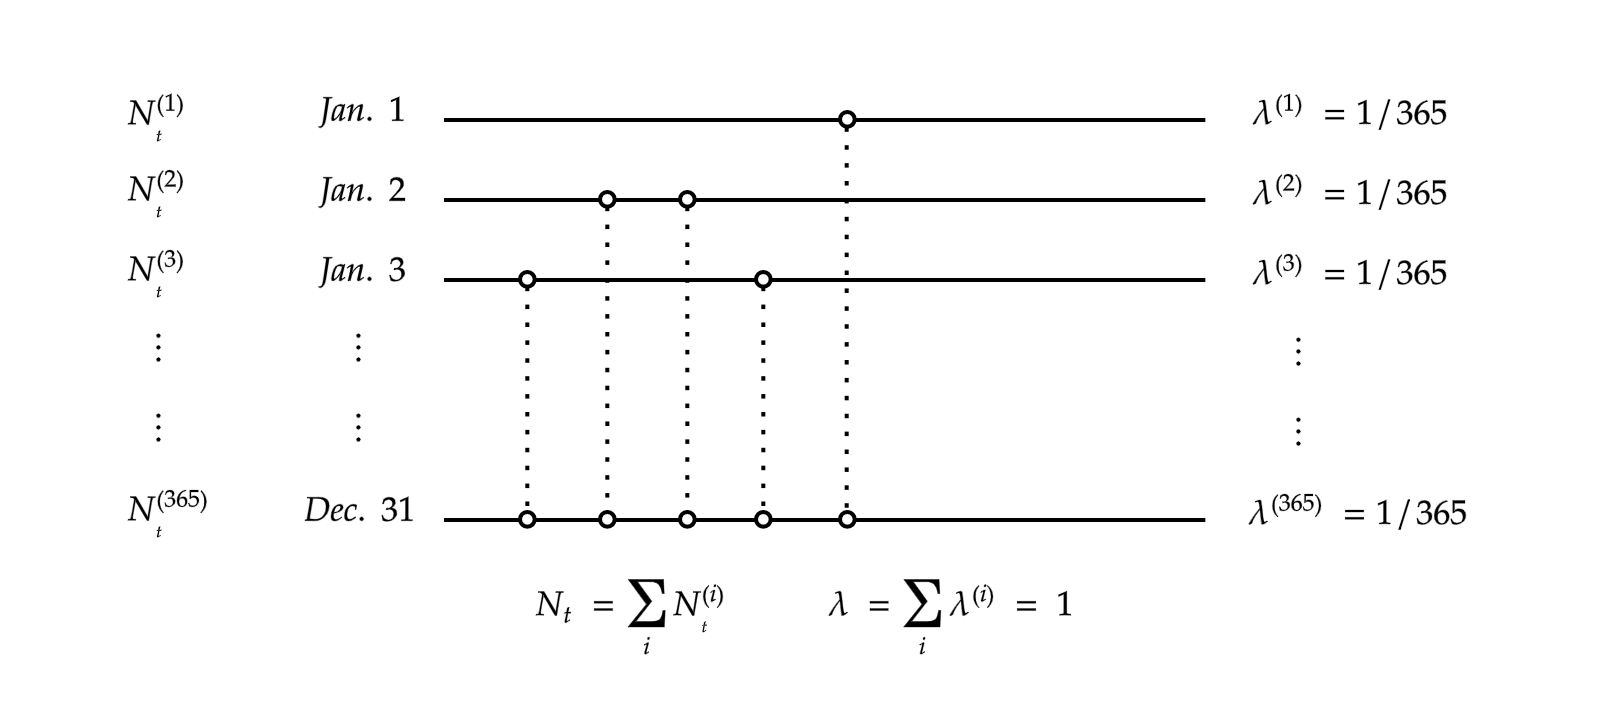
\includegraphics[width=\textwidth]{fig-21.png}
  \end{center}
  Let $(X_i)_{i \geq 0}$ be the interarrival sequence for the process of people entering the room. The $X_i$ are i.i.d exponential with mean 1. Let $T$ be the first time when two people in the room share the same birthday. If $K$ people are in the room at that time,
  \[T=\sum_{i=1}^{K} X_{i}\]
  \noindent $(X_i)$ is independent of $K$. Taking the expectation,
  \[\mathbb{E}[T] = \mathbb{E}[K] \cdot \underbrace{\mathbb{E}[X_1]}_{= 1} = \mathbb{E}[K]\]
  \noindent Let $Z_k$ be the time when the second person marked with birthday $k$ enters the room. Then, the first time that two people in the room have the same birthday is,
  \[T = \min_{1 \leq k \leq 365} Z_k\]
  \noindent Equivalently, \text{$Z_k$} is the arrival time of the second event of a Poisson process. Moreover, \text{$Z_k$} has a gamma distribution with parameters and density,
  \[n = 2 \quad \quad \lambda = \frac{1}{365} \quad \quad f(t)=\frac{t e^{-t / 365}}{365^{2}} (t>0)\]
  \noindent The cumulative distribution function is,
  \[P\left(Z_{1} \leq t\right)=\int_{0}^{t} \frac{s e^{-s / 365}}{365^{2}} d s=1-\frac{e^{-t / 365}(365+t)}{365}\]
  \noindent This gives,
  \begin{align*}
    P(T > t) &= P\bigg(\min_{1 \leq k \leq 365} Z_k > t\bigg) \\
             &= P(Z_1 > t, \cdots, Z_{365} > t) \\
             &= P\left(Z_{1}>t\right)^{365} \\
             &= \left(1+\frac{t}{265}\right)^{365} e^{-t} \quad (t > 0)
  \end{align*}
  \noindent Therefore, the desired birthday expectation is,
  \[E(K)=E(T)=\int_{0}^{\infty} P(T>t) d t=\int_{0}^{\infty}\left(1+\frac{t}{365}\right)^{365} e^{-t} d t\]
\end{ex}

\subsection{Poissonization and Depoissonization}
Poisson processes can be used to prove theorems for discrete time processes. Given $(X_k)_{k \geq 0}$, do the following:
\begin{enumerate}
  \item \textbf{(Poissonize)} Let $X_t^* = X_{N_t}$ for a Poisson process $(N_t)_{t \geq 0}$ to embed the discrete time process $(X_k)$ in continuous time.
  \item \textbf{(Analyze)} Show that $X^*_t$ has the desired property.
  \item \textbf{(Depoissonize)} Transfer the chain to the discrete time process.
\end{enumerate}

\begin{thm}[Recurrence via Poissonization]
  Let $(X_k)_{k \geq 0}$ be a time-homogeneous Markov chain. If $(N_t)_{t \geq 0}$ is a Poisson process with $\lambda = 1$, then a state $x$ is \textbf{recurrent} if and only if,
  \[\int_{0}^{\infty} P\left(X_{N_{t}}=x\right) d t=\infty\]
\end{thm}

\begin{proof}
  It suffices to show the following,
  \[\int_{0}^{\infty} P\left(X_{N_{t}}=x\right) d t = \sum_{k=0}^{\infty} p_k(x,x)\]
  \noindent Since $P\left(X_{k}=x\right) = P\left(X_{N_{t}}=x \mid N_{t}=k\right)$,
  \begin{align*}
    \int_{0}^{\infty} P\left(X_{N_{t}}=x\right) d t 
    &= \int_{0}^{\infty} \sum_{k=0}^{\infty} P(N_t = x) \cdot P\left(X_{N_{t}}=x \mid N_{t}=k\right) d t \\
    &= \sum_{k=0}^{\infty} P\left(X_{N_{t}}=x \mid N_{t}=k\right) \cdot \int_{0}^{\infty} P(N_t = x) d t \\
    &= \sum_{k=0}^{\infty} P\left(X_{k}=x\right) \cdot \int_{0}^{\infty} P(N_t = x) d t \\
    &= \sum_{k=0}^{\infty} p_k(x,x) \cdot \underbrace{\int_{0}^{\infty} \frac{e^{-t} t^{k}}{k !} d t}_{= 1} \\
      &=\sum_{k=0}^{\infty} p_k(x,x) \\
  \end{align*}
\end{proof}

\begin{ex}{Poissonized Simple Random Walk on $\mathbb{Z}$}{label}
  Let $(X_k)_{k \geq 0}$ be a simple random walk on $\mathbb{Z}^d$.
    \begin{enumerate}
    \item \textbf{(Poissonize)} Let $(N_t)$ be a Poisson process with \text{$\lambda = 1$}. Assume that each arrival is marked \text{$"L_t"$} if the chain moves to the left, and \text{$"R_t"$} if the chain moves to the right. Then,
    \begin{align*}
      &(N_t^{(L_t)})_{t \geq 0} \sim \text{Po}\left(\frac{\lambda \cdot t}{2}\right) = \text{Po}\left(\frac{t}{2}\right) \\
      &(N_t^{(R_t)})_{t \geq 0} \sim \text{Po}\left(\frac{\lambda \cdot t}{2}\right) = \text{Po}\left(\frac{t}{2}\right)
    \end{align*}
    \noindent Moreover, $(N_t^{(L_t)})$ and $(N_t^{(R_t)})$ are independent. Thus,
    \[X^*_t := X_{N_t} =  (N_t^{(R_t)})_{t \geq 0} - (N_t^{(L_t)})_{t \geq 0} \sim \underbrace{\text{Po}\bigg(\frac{t}{2}\bigg)}_{+1 ("R_t")} - \underbrace{\text{Po}\bigg(\frac{t}{2}\bigg)}_{-1 ("L_t")}\]

    \item \textbf{(Analyze)} We want to determine if $X^*_t$ is recurrent,
    \begin{align*}
      P\left(X_{N_{t}}=0\right) &= P(L_t = R_t) \\
                                  &= \sum_k^{\infty} P(L_t = k \mid R_t = k) \cdot P(R_t = k) \\
                                  &= \sum_{k=0}^{\infty}\left(\frac{e^{-t / 2}(t / 2)^{k}}{(k !)}\right)^{2} \quad \text{ by independence} \\
                                  &= e^{-t} \cdot \mathcal{I}_0(t) \quad \text{where $\mathcal{I}_0(t)$ is the Bessel function}
    \end{align*}
    \noindent Therefore, $P(X_{N_t} = 0) \cdot \sqrt{2\pi t} \rightarrow 1$ as $t \rightarrow \infty$ using the Stirling Formula or Bessel function properties. Consequently,
    \[\int_{0}^{\infty} P\left(X_{N_{t}}=0\right) d t=\infty \quad \text { because } \quad \int_{1}^{\infty} \frac{d t}{\sqrt{2 \pi t}}=\infty\]
    \item \textbf{(Depoissonize)} Apply "Recurrence via Depoissonization".
  \end{enumerate}
\end{ex}

\begin{ex}{Poissonized Simple Random Walk on $\mathbb{Z}^d$}{label}
  Let $(X_k)_{k \geq 0}$ be a simple random walk on $\mathbb{Z}^d$.
  \begin{enumerate}
    \item \textbf{(Poissonize)} Let \text{$(N_t)$} be a Poisson process with \text{$\lambda = 1$}. Applying Thinning as in the example on \text{$\mathbb{Z}$},
      \[X^*_k := X_{N_t} = \bigg( X_{N_t}^{(1)}, \cdots, X_{N_t}^{(d)} \bigg)\]
    \noindent where $(X_{N_t}^{(i)})$ and $(X_{N_t}^{(j)})$ are independent if $i \neq j$, and,
    \[(X_{N_t}^{(i)}) \sim \text{Po}\left(\frac{t}{d}\right) \quad \text{ for all $i \in [n]$}\]
    \item \textbf{(Analyze)} We want to determine if $X^*_t$ is recurrent,
      \begin{align*}
    P\left(X_{N_{t}}=\Vec{0}\right)&=P\left(X_{N_{t}}^{(1)}=0\right)^{d} \text{ by independence}\\
    &= \left(\sum_{k=0}^{\infty}\left(\frac{e^{-t / 2 d}(t / 2 d)^{k}}{(k !)}\right)^{2}\right)^d
  \end{align*}
  \noindent Therefore, $\int_{1}^{\infty}\left(\frac{1}{\sqrt{2 \pi t / d}}\right)^{d} d t<\infty \text { if and only if } d \geq 3$ as
  \[
  \bigg(\sqrt{\frac{2 \pi t}{d}}\bigg)^{d} \cdot P\left(X_{N_{t}}=\Vec{0}\right) \rightarrow 1
  \]
  \item \textbf{(Depoissonize)} Apply "Recurrence via Poissonization".
  \end{enumerate}
\end{ex}

\subsection{Order Statistics}
If a Poisson process contains exactly $n$ events in $[0, t]$, then the unordered times of those events are uniformly distributed on $[0, t]$.

\begin{rmk}[Conditional on 1 Event]
  $P\left(S_{1} \leq s \mid N_{t}=1\right) = \frac{s}{t}$.
\end{rmk}

\begin{proof}
  Using the definition of Conditional Probability,
  \begin{align*}
  P\left(S_{1} \leq s \mid N_{t}=1\right) &=\frac{P\left(S_{1} \leq s, N_{t}=1\right)}{P\left(N_{t}=1\right)} \\
  &=\frac{P\left(N_{s}=1, N_{t}=1\right)}{P\left(N_{t}=1\right)} \\
  &=\frac{P\left(N_{s}=1, N_{t}-N_{s}=0\right)}{P\left(N_{t}=1\right)} \\
  &=\frac{P\left(N_{s}=1\right) \cdot P\left(N_{t-s}=0\right)}{P\left(N_{t}=1\right)}\\
  &=\frac{e^{-\lambda s} \lambda s e^{-\lambda(t-s)}}{e^{-\lambda t} \lambda t}\\
  &=\frac{s}{t}
  \end{align*}
  \noindent since $N_{t-s} \sim \text{Po}(\lambda \cdot (t-s))$.
\end{proof}

\begin{defn}[Order Statistic]
  Let $U_1, \cdots, U_n$ be an i.i.d sequence of Unif$([0,t])$ random variables. Their joint density function is,
  \[f_{U_{1}, \ldots, U_{n}}\left(u_{1}, \ldots, u_{n}\right)=\frac{1}{t^{n}}\]
  \noindent for $0 \leq u_{1}, \ldots, u_{n} \leq t$. Arrange $U_i$ in increasing order,
  \[U_{(1)} \leq U_{(2)} \leq \cdots \leq U_{(n)}\]
  \noindent $U_(k)$ is the $k$th smallest of the $U_i$. The ordered sequence,
  \[\left(U_{(1)}, \ldots, U_{(n)}\right)\]
  \noindent is the \textbf{order statistics} of the original sequence. Its joint density is,
  \[f_{U_{(1)}, \ldots, U_{(n)}}\left(u_{1}, \ldots, u_{n}\right)=\frac{n !}{t^{n}}\]
  \noindent $0 \leq u_{1}<\cdots<u_{n} \leq t$.
\end{defn}

\begin{thm}[Order Statistics via Poissonization]
  Let $S_1, S_2, \cdots$ be the arrival times of a Poisson process with parameter $\lambda$. Conditional on $N_t = n$, the joint distribution of $(S_1, \cdots, S_n)$ is the distribution of the order statistics of $n$ i.i.d uniform random variables on $[0,t]$.
  \[f\left(s_{1}, \ldots, s_{n}\right)=\frac{n !}{t^{n}}\]
  \noindent for $0<s_{1}<\cdots<s_{n}<t$. Equivalently, let $U_1, \cdots, U_n$ be an i.i.d sequence of Unif$([0,t])$ random variables. Then, conditional on $N_t = n$, 
  \[\left(S_{1}, \ldots, S_{n}\right) \text { and } \left(U_{(1)}, \ldots, U_{(n)}\right)\]
  \noindent have the same distribution.
\end{thm}

\begin{proof}
  See Dobrow 6.5 (p.245).
\end{proof}

\begin{cor}
  Results for arrival times offer a new method for simulating a Poisson process with parameter $\lambda$ on an interval $[0, t]$:
  \begin{enumerate}
    \item Simulate the number of arrivals $N$ in $[0,t]$ from Po$(\lambda \cdot t)$
    \item Generate $N$ i.i.d random variables uniformly distributed on $(0,t)$
    \item Sort the variables in increasing order to give the Poisson arrival times
  \end{enumerate}
\end{cor}

\subsection{Spatial Poisson Processes}
The spatial Poisson process is a model for the distribution of events in a two- or higher-dimensional space\footnote{The uniform distribution arises for the spatial process in a similar way to how it does for the one-dimensional Poisson process. Given a bounded set $A \subseteq \mathbb{R}^d$, conditional on there being $n$ points in $A$, the location of the points are uniformly distributed on $A$.}. For $d \geq 1$ and $A \subseteq \mathbb{R}^d$, let $N_A$ denote the number of points in the set $A$. We write $|A|$ for the size of $A$ (i.e., area in $\mathbb{R}^2$ and volume in $\mathbb{R}^3$).

\begin{defn}[Spatial Poisson Process]
  A collection of random variables $(N_A)_{A \subseteq \mathbb{R}^d}$ is a \textbf{spatial Poisson process} with parameter $\lambda$ if,
  \begin{enumerate}
    \item $N_A \sim \text{Po}(\lambda \cdot |A|)$ for each bounded set $A \subseteq \mathbb{R}^d$
    \item $N_A$ and $N_B$ are independent random variables if $A$ and $B$ are disjoint
  \end{enumerate}
\end{defn}

The definition of a spatial Poisson process can be generalized to a Poisson random measure as follows,
\begin{defn}[Poisson Random Measure]
  The \textbf{Poisson random measure} is the unique function $N: \mathcal{B} \rightarrow \mathbb{N}_0$ so that for any $A \in \mathcal{B}$,
  \begin{enumerate}
    \item If $N_A$ is the number of points in $A$, then,
    \[N_A \sim \text{Po}\left(\int_A f(x) d x\right)\]
    \item If $A_1, \cdots, A_k \in \mathcal{B}$ are disjoint, compact sets,
    \[\left(N(A_1), N(A_2), \cdots, N(A_k)\right)\]
    \noindent are independent, Poisson distributed random variables with parameters,
    \[\int_{A_j} f(x) d x \quad 1 \leq j \leq k\]
  \end{enumerate}
  \noindent where $f: \mathbb{R}^d \rightarrow \mathbb{R}$ is called the "intensity" of the process.
\end{defn}

\begin{marginfigure}
 \begin{center}
      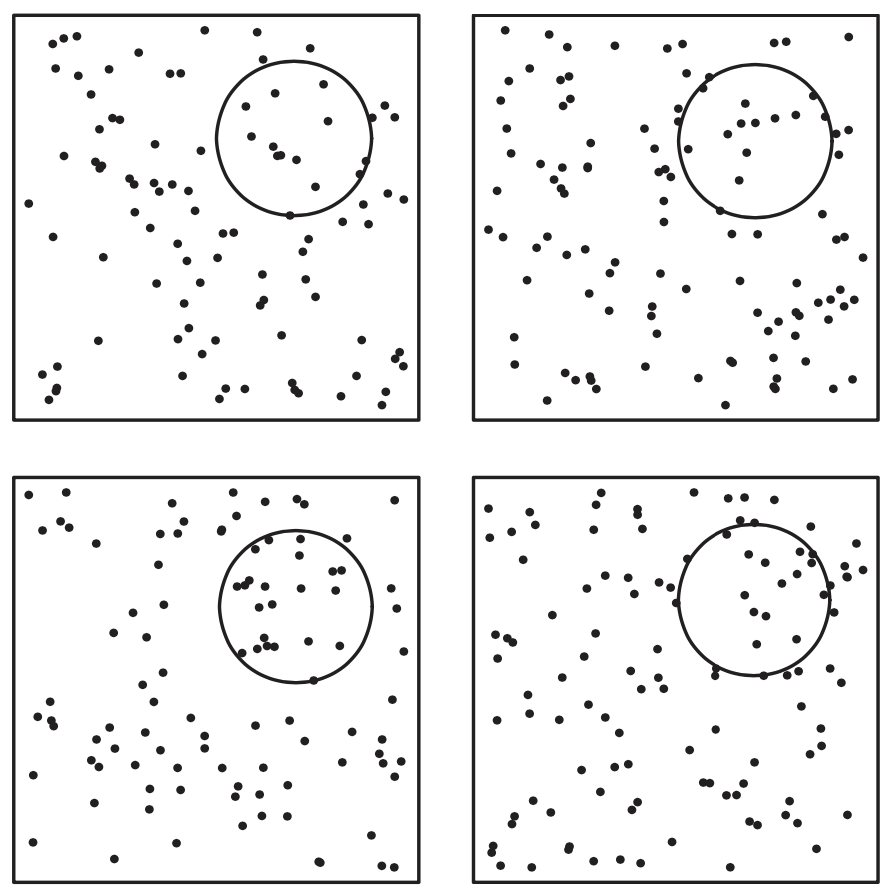
\includegraphics[width=\textwidth]{fig-22.png}
      \caption{Samples of a spatial Poisson process with parameter $\lambda = 100$ on the square $[0,1] \times [0,1]$.}
  \end{center}
\end{marginfigure}

\begin{rmk}
  Let $f: \mathbb{R}^d \rightarrow \mathbb{R}$ be a continuous, non-negative function.
  \begin{enumerate}
    \item \textbf{(Number of Points in $I$)} For any closed rectangle $I \subset \mathbb{R}^d$,
    \[N_I \sim \text{Po}\left(\int_I f(x) d x\right)\]
    \item \textbf{(Location of Points in $I$)} Define an i.i.d collection $X_I$ of points,
    \[(X_j)_{j \in [1,N_I]} \quad \text{ with } \quad X_j \sim P(X_j \in B) = \frac{\int_B f(x) d x}{\int_I f(x) d x}\]
    \item \textbf{(Spread of Points in $\mathbb{R}^d$)} Repeat over a partition into rectangles,
    \[X = \cup_I X_I \quad \text{ and } \quad N_A := |\{X \cap A\}| \quad \text{for each $A \in \mathcal{B}$}\]
  \end{enumerate}
  \noindent $N$ is a Poisson random measure with intensity $f$\footnote{
  \textbf{Notes on Spatial Processes:}
  \begin{enumerate}
    \item If $d = 1$ and $f$ is constant at $\lambda > 0$, then $N_{[0,t]} \leftrightarrow N_t$ is the Poisson process with rate $\lambda$.
    \item If $d > 1$ and $f$ is constant at $\lambda > 0$, then this is the homogeneous spatial Poisson process.
  \end{enumerate}
  }.
\end{rmk}

\begin{defn}[Non-Homogeneous Poisson Process]
  A counting process $(N_t)_{t \geq 0}$ is \textbf{non-homogeneous Poisson} with intensity $\lambda(t)$ if,
  \begin{enumerate}
    \item $N_0 = 0$
    \item For all $t > 0$, $N_t$ has a Poisson distribution with mean,
    \[E\left(N_{t}\right)=\int_{0}^{t} \lambda(x) d x\]
    \item For $0 \leq q < r \leq s < t$. $N_r - N_q$ and $N_t - N_s$ are independent
  \end{enumerate}
\end{defn}

\section{Continuous-Time Markov Chains}
\subsection{Holding Times}
\begin{defn}[Continuous-Time Markov Property]
  The \textbf{Markov property} for continuous-time chains $(X_t)_{t \geq 0}$ with discrete state space $S$ is,
  \[P\left(X_{t}=j \mid \left(X_{u}\right)_{0 \leq u < s} \text{ and } X_{s}=i\right)=P\left(X_{t}=j \mid X_{s}=i\right)\]
  \noindent for all $t \geq s$ and states $i, j \in S$.
\end{defn}

\begin{defn}[Time-Homogeneous]
  A continuous-time Markov chain $(X_t)_{t \geq 0}$ with discrete state space $S$ is \textbf{time-homogeneous} if,
  \[P\left(X_{t+s}=j \mid X_{s}=i\right) = P\left(X_{t}=j \mid X_{0}=i\right)\]
  \noindent for $s \geq 0$. The transition probabilities can be arranged in a function,
  \[\mathbf{P}_{i j}(t)=P\left(X_{t}=j \mid X_{0}=i\right)\]
  \noindent which is the analog of $p_t(i,j)$ in the discrete setting\footnote{$\mathbf{P}(t)$ is not the transition matrix $\tilde{\mathbf{P}}$ of the embedded chain, since $t \in \mathbb{R}$.}.
\end{defn}

\begin{defn}[Chapman-Kolmogorov]
  A continuous-time Markov chain $(X_t)_{t \geq 0}$ with transition function $\mathbf{P}(t)$ satisfies that,
  \[\mathbf{P}(s + t) = \mathbf{P}(s) \cdot \mathbf{P}(t) \text{ for $s, t \geq 0$.}\]
\end{defn}

\begin{proof}
  By conditioning on $X_s$, 
  \begin{align*}
    \boldsymbol{P}_{i j}(s+t) &=P\left(X_{s+t}=j \mid X_{0}=i\right) \\
    &=\sum_{k} P\left(X_{s+t}=j \mid X_{s}=k, X_{0}=i\right) \cdot P\left(X_{s}=k \mid X_{0}=i\right) \\
    &=\sum_{k} P\left(X_{s+t}=j \mid X_{s}=k\right) \cdot P\left(X_{s}=k \mid X_{0}=i\right) \\
    &=\sum_{k} P\left(X_{t}=j \mid X_{0}=k\right) \cdot P\left(X_{s}=k \mid X_{0}=i\right) \\
    &=\sum_{k} P_{i k}(s) \cdot P_{k j}(t) \\
    &=[\mathbf{P}(s) \cdot \mathbf{P}(t)]_{i j}
    \end{align*}
\end{proof}

\begin{defn}[Holding Time]
  The \textbf{holding time} $T_i$ at a state $i$ is the length of time that a continuous-time Markov chain started in $i$ stays in $i$ before transitioning to a new state.
\end{defn}

\begin{thm}
  Let $T_i$ be the holding time at state $i$. Then $T_i \sim \text{Exp}(\lambda_i)$.
\end{thm}

\begin{proof}
  The exponential distribution is the only continuous distribution that is memoryless, so it suffices to prove that $T_i$ is memoryless. Let $s, t \geq 0$. Suppose that the chain starts in $i$. Then,
  \[\{T_i > s\} = \{X_u = i \text{ for } u \in [0,s]\}\]
  \noindent Moreover, $\{T_i > s + t\}$ implies that $\{T_i > s\}$, so,
  \[P(T_i > s + t \mid X_0 = i) = P(\underbrace{\{T_i > s + t\}}_{A} \cap \underbrace{\{T_i > s\}}_{B} \mid X_0 = i)\]
  \noindent Applying Bayes' Law with the conditional probability measure,
  \[P(A \cap B \mid X_0 = i) = P(A \mid B \cap \{X_0 = i\}) \cdot P(B \mid X_0 = i)\]
  \noindent and using homogeneity and the Markov property,
  \begin{align*}
    &= P(T_i > s + t \mid \{T_i > s\} \cap \{X_0 = i\}) \cdot P(T_i > s \mid X_0 = i) \\
    &=P\left(T_{i}>s+t \mid X_{u}=i \text { for } u \in [0,s] \right) \cdot P\left(T_{i}>s \mid X_{0}=i\right) \\
    &=P\left(T_{i}>s+t \mid X_{s}=i\right) \cdot P\left(T_{i}>s \mid X_{0}=i\right) \\
    &=P\left(T_{i}>t \mid X_{0}=i\right) \cdot P\left(T_{i}>s \mid X_{0}=i\right)
  \end{align*}
  \noindent shows that $T_i$ satisfies the definition of memoryless,
  \[P(T_i > s + t \mid X_0 = i) = P\left(T_{i}>t \mid X_{0}=i\right) \cdot P\left(T_{i}>s \mid X_{0}=i\right)\]
\end{proof}

\begin{defn}[Absorbing State]
  A state $i$ is \textbf{absorbing} if the parameter of the exponential distribution for the holding time $T_i$ is zero,
  \[\mathbb{E}[T_i] = \frac{1}{0} = \infty\]
\end{defn}

\begin{defn}
  A continuous-time Markov chain is \textbf{explosive} at a time $t \in \mathbb{R}^+$ if there are infinitely-many transitions in all neighborhoods\footnote{In Dobrow, a state $i \in S$ is called explosive if the holding time parameter $\lambda_i$ of $T_i$ is infinite, i.e., \[\mathbb{E}[T_i] = \frac{1}{\infty} = 0\]},
  \[(t-\epsilon, t) \quad \text{ for } \epsilon > 0 \text{ arbitrary }\]
\end{defn}

The evolution of a continuous-time Markov chain which is neither absorbing nor explosive can be described as follows,
\begin{enumerate}
  \item Starting from $i$, the process stays in $i$ for an exponentially distributed length of time, which is $1 / q_i$ on average
  \item The chain hits a new state $j \neq i$, with probability $p_{ij}$
  \item The process stays in $j$ for an exponentially distributed length of time, which is $1 / q_j$ on average. It then hits a new state $l \neq j$
\end{enumerate}

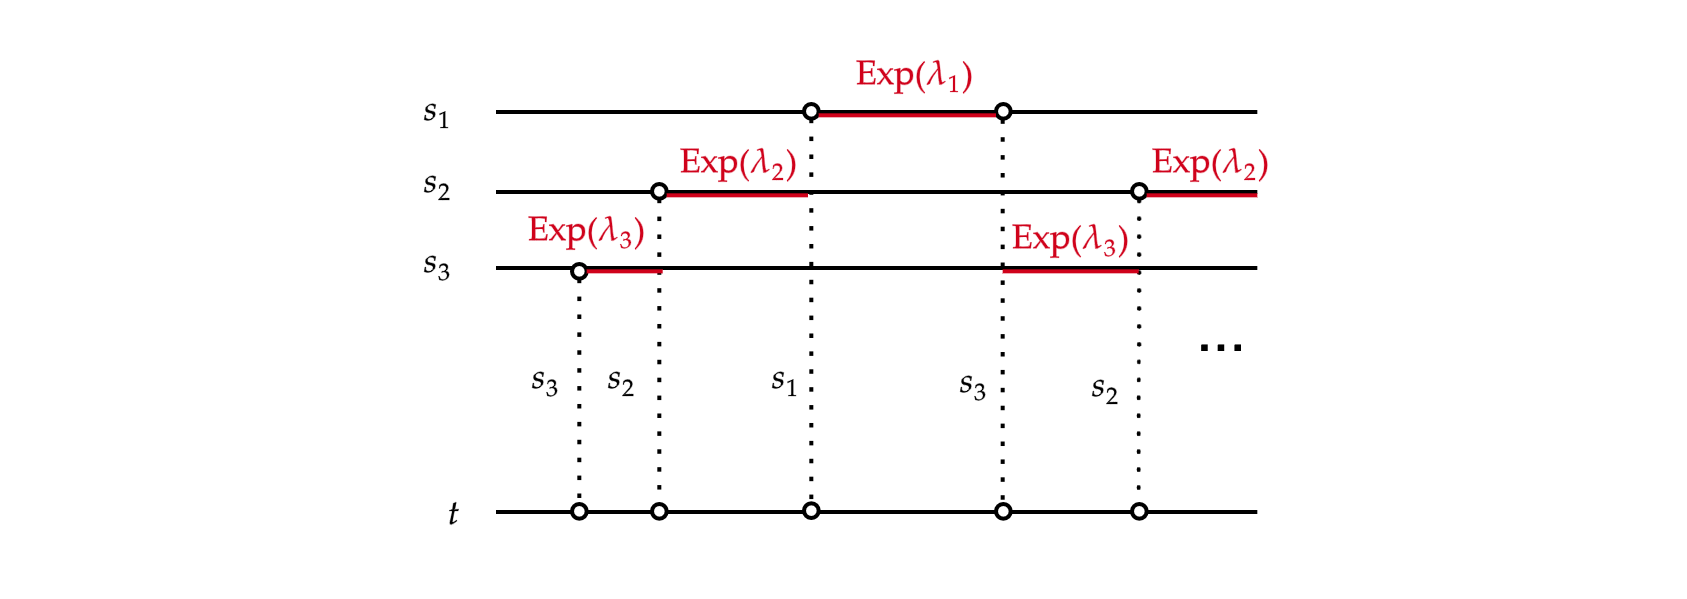
\includegraphics[width=\textwidth]{fig-25.png}

\begin{ex}{Continuous-Time Weather Chain}{label}
  Define the state space \text{$S = \{\texttt{rain}, \texttt{ snow}, \texttt{ clear}\}$}. Assume that,
  \begin{enumerate}
    \item Rain lasts, on average, 3 hours
    \item Snow lasts, on average, 6 hours
    \item Clear weather lasts, on average, 12 hours
  \end{enumerate}

  \begin{center}
    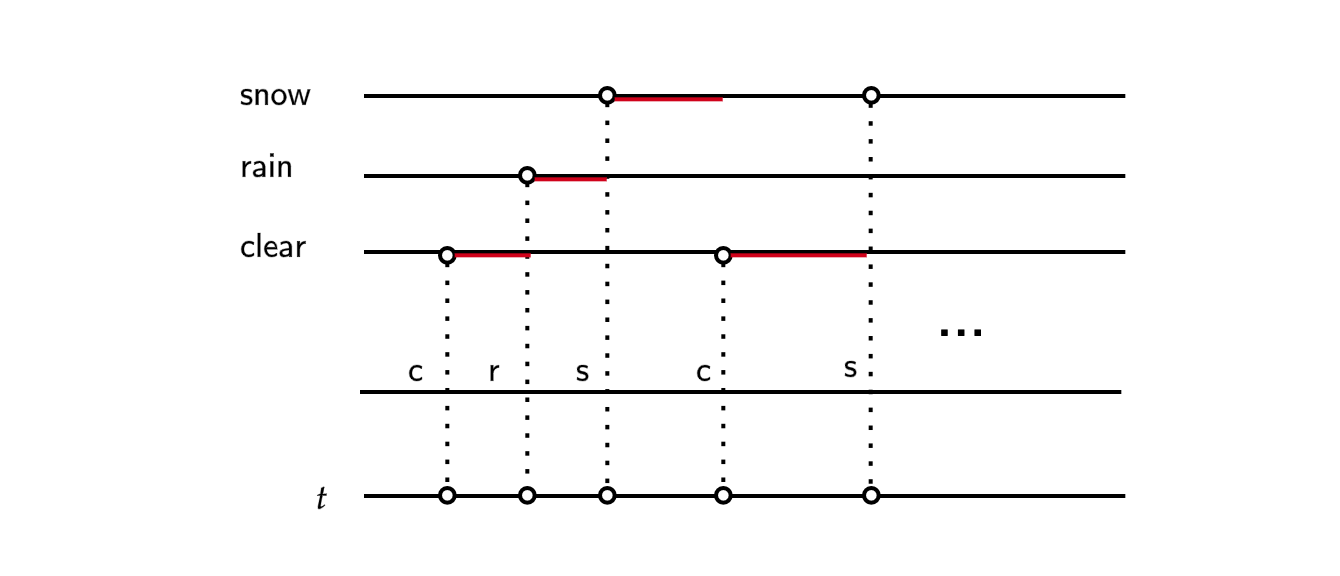
\includegraphics[width=\textwidth]{fig-23.png}
  \end{center}

  Changes in weather states are described by the matrix,
   \[\tilde{\boldsymbol{P}} = \begin{blockarray}{cccc}
    \texttt{rain} & \texttt{snow} & \texttt{clear} \\
    \begin{block}{(ccc)c}
      0 & 1/2 & 1/2 & \texttt{rain} \\
      3/4 & 0 & 1/4 & \texttt{snow} \\
      1/4 & 3/4 & 0 & \texttt{clear} \\
    \end{block}
    \end{blockarray}\]

  Let \text{$X_t$} be the weather at time \text{$t$}. Then, \text{$(X_t)_{t \geq 0}$} is a continuous-time Markov chain. Moreover, \text{$\tilde{\mathbf{P}}$}, as well as the exponential parameters \text{$(\lambda_r, \lambda_s, \lambda_c) = (1/3, 1/6, 1/12)$}, specify $\mathbf{P}(t)$, i.e., \text{$P\left(X_{t_{1}}=i_{1}, \ldots, X_{t_{n}}=i_{n}\right)$} for \text{$n \geq 1$}, states \text{$s_i$} and times \text{$t_i \geq 0$}.
\end{ex}

\begin{defn}[Embedded Chain]
  A sequence $(Y_k)_{k \geq 0}$ is the \textbf{embedded chain} of a continuous-time process $(X_k)$ if $Y_k$ is the $k$th state visited.
\end{defn}

\begin{rmk}
  The transition matrix $\tilde{\mathbf{P}}$ of the embedded chain of a continuous-time process is a stochastic matrix whose diagonal entries are zero\footnote{The process can never transition from state $i$ to state $i$. It remains in $i$ for an exponential amount of time, after which it transitions to another state $j$ ($j \neq i$).}.
\end{rmk}

A continuous-time Markov chain can also be described by specifying transition rates between pairs of states. Suppose that for for each state $i$, there are independent alarm clocks associated with each of the states that the process can visit after $i$. Then,
\begin{enumerate}
  \item If $j$ can be hit from $i$, the alarm $C_{ij}$ associated with $(i,j)$ will ring after an exponentially distributed length of time with parameter $q_{ij}$

  \item The minimum time for one $C_{ij}$ ($i \neq j$) to finish ringing is the minimum of independent exponentials, which was proven to be exponential with parameter $q_i = \sum_k q_{ik}$

  \item When the process first hits $i$, the clocks start simulataneously, where the first alarm that rings determines the next state

  \item If the $(i,j)$ clock rings first and the process moves to $j$, a new set of exponential alarm clocks are started with rates $q_{j1}, q_{j2}, \cdots$

\end{enumerate}

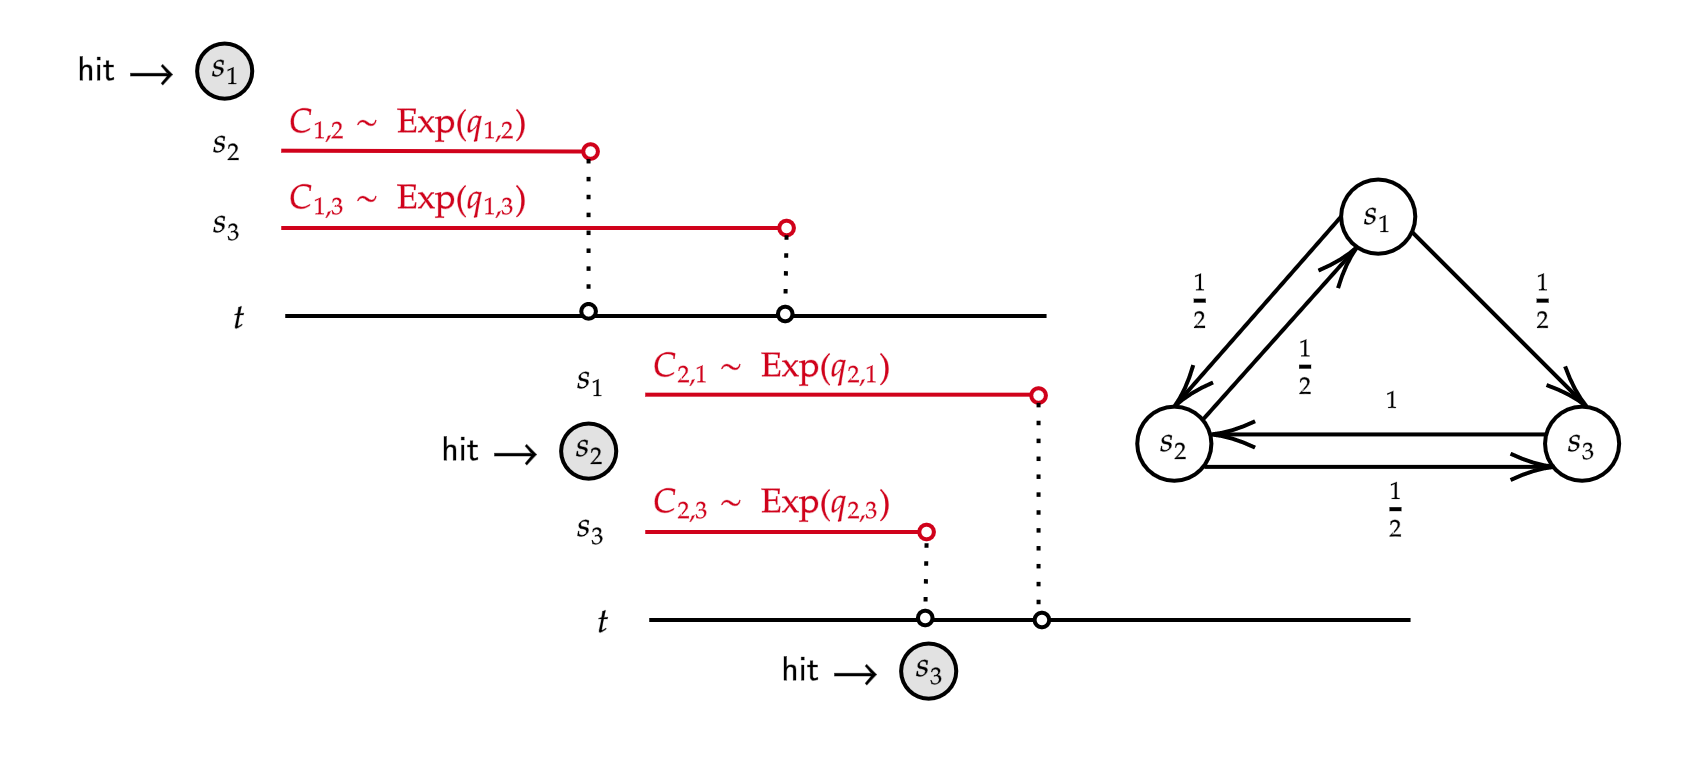
\includegraphics[width=\textwidth]{fig-24.png}

\subsection{Infinitesimal Generator}
\begin{defn}[Rate Matrix]
  The \textbf{rate matrix} $(\mathbf{Q})$ for a continuous-time Markov chain is defined as follows,
  \begin{align*}
    (\mathbf{Q})_{ij} &:= \begin{cases}
                        q_{i} \cdot \tilde{\mathbf{P}}_{ij} & i \neq j \\
                        0 & i = j
                      \end{cases} \\
                      &\hphantom{:}= \begin{cases}
                        q_{ij} \hphantom{ \cdot \tilde{\mathbf{P}}_{ij}} & i \neq j \\
                        0 & i = j
                      \end{cases}
  \end{align*}
\end{defn}

\begin{marginfigure}
  \textbf{Note on Generator Matrix:}

  \noindent A continuous-time Markov chain $(X_t)_{t \geq 0}$ with transition function $\mathbf{P}(t)$ and generator $\mathbf{Q}$ satisfies that,
  \begin{enumerate}
    \item $\mathbf{P}^{\prime}(t) = \mathbf{P}(t) \cdot \mathbf{Q}$
    \item $\mathbf{P}^{\prime}(t) = \mathbf{Q} \cdot \mathbf{P}(t)$
  \end{enumerate}
  \noindent These are called the "Kolmogorov Forward, Backward Equations".
\end{marginfigure}

\begin{defn}[Generator Matrix]
  The \textbf{generator matrix} $\mathbf{Q}$ for a continuous-time Markov chain is defined as follows\footnote{If the smallest signed value of a generator matrix \textbf{Q} is finite, then we say the chain is "bounded rate". Moreover, any finite chain is bounded rate.},
  \[
  \mathbf{Q}_{ij} := \begin{cases}
    q_{ij} & i \neq j \\
    \underbrace{-q_i}_{- \sum_{k} q_{ik}} & i = j
  \end{cases}
  \]
\end{defn}

\begin{cor}
  The generator is not a stochastic matrix. Diagonal entries are negative, entries can be greater than 1, and rows sum to 0.
\end{cor}

\begin{cor}
  A continuous-time Markov chain $(X_t)_{t \geq 0}$ satisfies that,
   \[
    \tilde{\boldsymbol{P}}_{i j} := \begin{cases}
    P\left(C_{i, j}=\hat{C}\right)=\frac{q_{i j}}{q_{i}}=\frac{q_{i j}}{\sum_{k} q_{ik}} & i \neq j \\
    0 & i = j
  \end{cases}
  \]
  \noindent where $\tilde{\boldsymbol{P}}$ is the embedded chain, and $\{C_{ij} = \hat{C}\}$ is the event that $C_{ij}$ is the first alarm that rings and determines the next state\footnote{The holding time parameters $\lambda_i$ are equal to $q_i$.}.
\end{cor}

\begin{cor}
  A continuous-time Markov chain $(X_t)_{t \geq 0}$ with transition function $\mathbf{P}(t)$ and generator $\mathbf{Q}$ satisfies that,
  \[\boldsymbol{P}(t)=e^{t \boldsymbol{Q}}=\sum_{n=0}^{\infty} \frac{1}{n !}(t \boldsymbol{Q})^{n}=\boldsymbol{I}+t \boldsymbol{Q}+\frac{t^{2}}{2} Q^{2}+\frac{t^{3}}{6} Q^{3}+\cdots\]
\end{cor}

\begin{marginfigure}
  \textbf{Note on Matrix Exponential:}

  \noindent Let $\mathbf{A}$ be a $k \times k$ matrix. Then, 
  \begin{align*}
    e^{A}&=\sum_{n=0}^{\infty} \frac{1}{n !} A^{n} \\
         &=I+A+\frac{1}{2} A^{2}+\cdots
  \end{align*}
\end{marginfigure}

\subsection{Classification of States}
For characterizing the states of a continuous-time Markov chain, the definitions of accessibility, communication, and irreducibility are defined as in the discrete case. For example,

\begin{defn}[Irreducible]
  A continuous-time Markov chain with transition function $\mathbf{P}(t)$ is \textbf{irreducible} if for all $i, j \in S$, 
  \[\mathbf{P}_{ij}(t) > 0 \text{ for some $t > 0$}\]
\end{defn}

\begin{lem}
  If $\mathbf{P}_{ij}(t) > 0$ for some $t > 0$, then $\mathbf{P}_{ij}(t) > 0$ for all $t > 0$.
\end{lem}

\begin{proof}
  Suppose that $\mathbf{P}_{ij}(t) > 0$ for some $t > 0$. Then there exists a path from $i$ to $j$ in the embedded chain, and, since the exponential distribution is continuous, for any time $s$ there is positive probability of reaching $j$ from $i$ in $s$ time units\footnote{Formally, for $s \geq 0$, this means that,
   \begin{enumerate}
    \item $\mathbf{P}_{ij}(t + s) > 0$
    \item $\mathbf{P}_{ij}(t - s) > 0$
  \end{enumerate}}. 
\end{proof}

\begin{cor}
  All states of a continuous-time Markov chain are aperiodic.
\end{cor}

% \begin{thm}
%   A finite-state continuous-time Markov chain is irreducible if the parameter $q_i$ of the holding time $T_i$ for a state $i$ is positive.
%  \end{thm}

\subsection{Stationary Distributions}
\begin{defn}[Stationary Distribution]
  A probability distribution $\Vec{\pi}$ is a \textbf{stationary probability distribution} for a continuous-time chain if\footnote{As in the discrete case, the limiting distribution, if it exists, is a stationary distribution. However, the converse is not necessarily true and depends on the class structure of the chain.},
  \[\Vec{\pi} = \Vec{\pi} \cdot \mathbf{P}(t)\]
\end{defn}

\begin{cor}
  The stationary distribution $\Vec{\pi}$ is not the same as the stationary distribution of the embedded chain, $\Vec{\psi}$\footnote{$\pi_i$ is the long-term proportion of \textbf{time} that the process spends in state $i$. Conversely, $\psi(i)$ is the long-term proportion of \textbf{transitions} that the process makes into state $i$.}. However, for all $j$, 
  \[\psi(j) = \frac{\pi_jq_j}{\sum_k \pi(k)q_k} \quad \pi_j = \frac{\psi(j) / q_j}{\sum_k \psi(k) / q_k}\]
\end{cor}

\begin{thm}[Fundamental Limit Theorem]
  Let $\left(X_{t}\right)_{t \geq 0}$ be a finite, irreducible, continuous-time Markov chain with transition function $\boldsymbol{P}(t)$. Then, there exists a unique stationary distribution $\Vec{\pi}$, which is the limiting distribution of the chain. That is, for all $j \in S$,
  \[\lim _{t \rightarrow \infty} \mathbf{P}_{i j}(t)=\pi_j \text { for all } i\]
  \noindent Equivalently,
  \[\lim _{t \rightarrow \infty} \boldsymbol{P}(t)=\boldsymbol{\Pi}\]
  \noindent where $\boldsymbol{\Pi}$ is a matrix all of whose rows are equal to $\Vec{\pi}$.
\end{thm}

\begin{proof}
  The proof of the Fundamental Limit Theorem is omitted.
\end{proof}

\begin{thm}
  A probability distribution $\Vec{\pi}$ is a stationary distribution of a continuous-time Markov chain with generator \textbf{Q} if and only if,
  \[\Vec{\pi}\mathbf{Q} = \Vec{0} \quad \iff \quad \sum_{i} \pi_{i} Q_{i j}=0 \text { for all } j \in S\]
\end{thm}

\begin{proof}
  Assume that $\Vec{\pi} = \Vec{\pi} \mathbf{P}(t)$ for all $t \geq 0$. Differentiating at $t = 0$,
  \[\Vec{0} = \Vec{\pi}\mathbf{P}^{\prime}(0) = \Vec{\pi}\mathbf{Q}\]
  \noindent Conversely, assume that $\Vec{\pi}\mathbf{Q} = \Vec{0}$. Right-multiplying by $\mathbf{P}(t)$,
  \[\Vec{0} = \Vec{\pi}\mathbf{Q}\mathbf{P}(t) = \Vec{\pi}\mathbf{P}^{\prime}(t) \text{ for $t \geq 0$}\]
  \noindent by the Kolmogorov backward equation. This implies that $\Vec{\pi}\mathbf{P}(t)$ is constant, that is, $\Vec{\pi}\mathbf{P}(t) = \Vec{\pi}\mathbf{P}(0)$ for all $t$. But $\mathbf{P}(0) = I$\footnote{Observe that,
  \[\mathbf{P}_{i j}(0) = P(X_t = j \mid X_0 = i) = \begin{cases}1, & \text { if } i=j \\ 0, & \text { if } i \neq j\end{cases}\]
  }, so,
  \[\Vec{\pi} \mathbf{P}(t) = \Vec{\pi} \mathbf{P}(0) = \Vec{\pi} I = \Vec{\pi}\]
\end{proof}

\subsection{Poisson Subordination}
 \begin{defn}[Subordination]
   Let $(N_t)_{t \geq 0}$ be a Poisson process with parameter $\lambda$. Let $(Y_t)_{t \geq 0}$ be a finite-state, irreducible, discrete-time process with transition matrix \textbf{R}. Define a continuous-time process $(X_t)_{t \geq 0}$ by $X_t := Y_{N_t}$\footnote{Transitions for the $X_t$ process occur at the arrival times of the Poisson process. From state $i$, the process holds an exponentially distributed amount of time with parameter $\lambda$, and then transitions to $j$ with probability $\mathbf{R}_{ij}$}. The process $(X_t)$ is \textbf{subordinated to a Poisson process}.
 \end{defn}

 \begin{rmk}
   Let $\mathbf{P}(t)$ be the transition function of $(X_t)$. Then,
   \begin{align*}
     \mathbf{P}_{ij}(t) &= P(X_t = j \mid X_0 = i) \\
                        &= \sum_{k=0}^{\infty} P\left(X_{t}=j \mid \{N_{t}=k\} \cap \{X_{0}=i\}\right) \cdot P\left(N_{t}=k \mid X_{0}=i\right) \\
                        &=\sum_{k=0}^{\infty} P\left(Y_{k}=j \mid \{N_{t}=k\} \cap \{X_{0}=i\}\right) \cdot P\left(N_{t}=k\right) \\
                        &=\sum_{k=0}^{\infty} P\left(Y_{k}=j \mid Y_{0}=i\right) \cdot P\left(N_{t}=k\right) \\
                        &=\sum_{k=0}^{\infty} \mathbf{R}_{i j}^{k} \cdot \frac{e^{-\lambda t}(\lambda t)^{k}}{k !}
   \end{align*}
 \end{rmk}

  We have just seen how to construct a continuous-time Markov chain from a discrete-time chain and a Poisson process. We will now see that many continuous-time chains can be represented as chains subordinated to a Poisson process.

   \begin{rmk}
    Let \textbf{Q} be the generator of a continuous-time Markov chain with holding time parameters $\{q_i\}$. If $q_i \leq \lambda$ for all $i$, then we can define,
    \[\mathbf{R} = \frac{1}{\lambda} \mathbf{Q} + \mathbf{I} \text{ where $\lambda = \max_i q_i$}\]
    \noindent which is a stochastic matrix. The transition function is,
    \begin{align*}
      \boldsymbol{P}(t) &=e^{t \boldsymbol{Q}}=e^{-\lambda t} e^{t \boldsymbol{Q}} e^{\lambda t}=e^{-\lambda t} e^{t(\boldsymbol{Q}+\lambda \boldsymbol{I})} \\
      &=e^{-\lambda t} \sum_{k=0}^{\infty} \frac{1}{k !} t^{k}(\boldsymbol{Q}+\lambda \boldsymbol{I})^{k} \\
      &=\sum_{k=0}^{\infty}\left(\frac{1}{\lambda} \boldsymbol{Q}+\boldsymbol{I}\right)^{k} \frac{e^{-\lambda t}(\lambda t)^{k}}{k !} \\
      &=\sum_{k=0}^{\infty} \boldsymbol{R}^{k} \frac{e^{-\lambda t}(\lambda t)^{k}}{k !}
    \end{align*}
    \noindent \textbf{R} is not the matrix of the embedded Markov chain:
    \[
    \tilde{\mathbf{P}}_{i j}= \begin{cases}q_{i j} / q_{i}, & \text { for } i \neq j \\ 0, & \text { for } i=j\end{cases} \quad \quad \mathbf{R}_{i j}= \begin{cases}q_{i j} / \lambda, & \text { for } i \neq j \\ 1-q_{i} / \lambda, & \text { for } i=j\end{cases}
    \]
  \end{rmk}

  \begin{marginfigure}
    \textbf{Note on Poisson Subordination: }
    \begin{enumerate}
      \item From state $i$, wait an exponential length of time with rate $\lambda$
      \item Flip a coin with $P(H) = \frac{q_i}{\lambda}$
      \item If heads, transition according to \textbf{R}. Otherwise, stay at $i$ and repeat
    \end{enumerate}
  \end{marginfigure}

\begin{thm}
  For a Markov chain subordinated to a Poisson process, the discrete $\mathbf{R}$-chain has the same stationary distribution as the original chain.
\end{thm}

\begin{proof}
  $\Vec{\pi} \mathbf{Q} =\Vec{\pi} \lambda(\boldsymbol{R}-\boldsymbol{I})=\lambda \Vec{\pi} \boldsymbol{R}-\lambda \Vec{\pi}$.
\end{proof}

\begin{cor}
  The following are equivalent,
  \begin{enumerate}
    \item $\Vec{\pi} \boldsymbol{P}(t) = \Vec{\pi}$ for all $t \geq 0$
    \item $\Vec{\pi} \boldsymbol{Q} = \Vec{0}$
    \item $\Vec{\pi} \tilde{\boldsymbol{R}} = \Vec{\pi}$ for some $\lambda = \max_i q_i$
  \end{enumerate}
\end{cor}

\begin{ex}{Totally Asymmetric Exclusion Process}{label}
  The dynamics of the \textbf{totally asymmetric simple exclusion process} on $\mathbb{Z}$ are as follows,
  \begin{enumerate}
    \item The alarm clock for a particle rings as a Poisson process of rate 1 at each site independently
    \item When the bell at site $i$ rings, if there is a particle at site $i$ and a hole at site $i - 1$, they exchange
  \end{enumerate}
  Equivalently, each particle in the system tries to jump to the left at rate 1, and the jump succeeds whenever the site to the left is unoccupied. Since it is possible for infinitely many particles to move instantaneously, and the minimum of infinitely-many exponential clocks is zero, there is no embedded chain and holding representation for this chain.
\end{ex}

\subsection{Birth-and-Death Chains}
\begin{marginfigure}
  \textbf{Note on Yule Process:}

  \noindent The Yule process ia a birth-and-death process in which the birth rate is $x \cdot \lambda$ and the death rate $0$.
\end{marginfigure}

\begin{defn}[Yule Process]
  Let $Y_t$ be the population size at time $t$. The \textbf{Yule process} $(Y_t)_{t \geq 0}$ is a continuous-time branching process where\footnote{The rate represents the expected time until the next division. Thus, $P(\min \{C_1, \cdots, C_x\} > t) = e^{-x \beta}$.},
  \begin{enumerate}
    \item $Y_0 = 1$, and the rate of the process is $q_{x, x + 1} = x \cdot \beta$
    \item Each individual gives birth to an offspring at a constant rate $\beta$
    \item Each individual gives birth independently of other individuals
    \item The distribution of each division time is Exp($\beta$)
  \end{enumerate}
\end{defn}

\begin{rmk}
  A Yule process $(Y_t)_{t \geq 0}$ satisfies the following identity,
  \[Y_{t + \tau} \sim Y_t^{(1)} + Y_t^{(2)} \quad \text{ and } \quad \tau \sim \text{Exp}(\beta)\]
  \noindent where $\tau$ is the time of the first division, and $Y_t^{(1)}, Y_t^{(2)}$ are Yule processes.
\end{rmk}

\begin{marginfigure}
  $(Y_t)$ cannot be written as a Poisson subordinated discrete time walk. However, it exists for all time without exploding. Conversely, if $q_{x, x+1} = \beta \cdot x^2$, then the process explodes in finite time.
\end{marginfigure}

\begin{rmk}
  Define the following,
  \begin{align*}
    &\text{Arrival $i$ is the birth of member $i+1$ of the population} \\
    &\text{$\hat{C}_i$ is the minimum time for one $C_i$ to finish ringing} \\
    &\text{$Z_i$ is the time of arrival $i$} \\
    &\text{$T_n := \min \{t \mid Y_t = n\}$}
  \end{align*}
  \noindent We need to compute $P(T_n \leq t)$,
  \begin{align*}
    P(T_n \leq t)
    &= P\left(\sum_{i=1}^{n-1} \hat{C}_i \leq t\right) \text{ where } \hat{C}_i \sim \text{Exp}(i \cdot \beta) \\
    &= P\left(\bigcap_{i=1}^{n-1} \{Z_i \leq t\}\right) \text{ where } Z_i \sim \text{Exp}(\beta)\\
    &= \prod_{i=1}^{n-1} P(Z_i \leq t) \text{ since $(Z_i)_{i \in [n-1]}$ i.i.d} \\
    &= (1 - e^{-t\beta})^{n-1} \text{ by induction}
  \end{align*}
\end{rmk}

\begin{rmk}
  We can write $Y_t = \sum_{i=1}^{\infty} \mathbbm{1}_{\{T_j \leq t\}}$. Then,
  \[\mathbb{E}[Y_t] = \mathbb{E}\left[\sum_{i=1}^{\infty} \mathbbm{1}_{\{T_j \leq t\}} \right] = \sum_{i=1}^{\infty} P(T_j \leq t) = \sum_{i=1}^{\infty} \left(1 - e^{-t \cdot \beta}\right)^{i-1} = e^{t \cdot \beta}\]
  \noindent using the sum of a geometric series.
\end{rmk}

\begin{defn}[Birth-and-Death]
  \textbf{Birth-and-death processes} are a class of time-reversible, continuous-time Markov chains. They satisfy,
  \begin{enumerate}
    \item Births occur from $i$ to $i + 1$ with rate $\beta$
    \item Deaths occur from $i$ to $i - 1$ with rate $1$
  \end{enumerate}
  \noindent making $q_{x, x+1} = \beta \cdot x$ and $q_{x, x-1} = x$\footnote{This represents an exponential 1 clock and a population of size $x$.}.
\end{defn}

\begin{marginfigure}
  The following questions are equivalent,
  \begin{enumerate}
    \item How many times is the Exp($\beta$) birth clock $C$ of an individual the minimum before the Exp($1$) death clock rings?
    \item How many offspring does the individual produce?
  \end{enumerate}
\end{marginfigure}

\begin{thm}
  If $\beta > 1$, then the probability of extinction is less than 1.
\end{thm}

\begin{proof}
  The proof is by a Poisson Process argument, where,
  \[\left(\frac{\beta}{1 + \beta}\right) \quad \text{ and } \quad \left(\frac{1}{1 + \beta}\right)\]
  \noindent are the parameters of each thinned process. Computing the number of divisions before death gives that $\mathbb{E}[Y] = \beta$.
\end{proof}

\begin{cor}
  Let $(Y_t)$ be a birth-and-death process with birth rate $\beta$ and death rate $1$. If $\beta \leq 1$, the underlying branching process goes extinct,
  \[Y_{t} \underset{t \rightarrow \infty}{\stackrel{a . s}{\longrightarrow}} 0 \quad \text{where $0$ is an absorbing state}\]
  \noindent Conversely, when $\beta > 1$, there exists a random variable $Y_{\infty}$,
  \[Y_{t} \underset{t \rightarrow \infty}{\stackrel{a . s}{\rightarrow}} Y_{\infty}\]
  \noindent and $P(Y_{\infty} = 0)$ is the extinction probability of the branching process,
  \[P(Y_{\infty} = \infty) = 1 - P(Y_{\infty} = 0)\]
\end{cor}

\begin{defn}
  Let $(Y_t)$ be an irreducible continuous-time Markov chain. $(Y_t)$ is null-recurrent if and only if $\mathbb{E}[\tau_0^+] = \infty$\footnote{Otherwise, $(Y_t)$ is positive-recurrent. This definition is the same as the discrete case.}.
\end{defn}

\begin{cor}
  The underlying discrete-time behavior does not determine positive or null recurrence for the chain. The holding time parameters can be made sufficiently large to see this.
\end{cor}

\begin{thm}
  An irreducible, continuous-time Markov chain is positive recurrent if and only if there exists a stationary probability vector $\Vec{\pi}$. That is, $\sum_{i \in S} \pi_i = 1$ and $\Vec{\pi} \mathbf{Q} = 0$, where $\mathbf{Q}$ is the generator of the chain.
\end{thm}

\begin{proof}
  The proof uses Martingales, and it was not seen in class.
\end{proof}

\begin{ex}{Reflected Birth-and-Death Chain}{label}
  We can modify the birth-and-death chain to make the boundary condition at zero reflect. Equivantly, we define,
  \[
  \mathbf{Q}^{\prime}_{x,y} = \begin{cases}
                        q_{x,y} & x \neq 0 \\
                        1 & x = 0 \text{ and } y \neq 0 \\
                        0 & x = 0 \text{ and } y = 0 \\
                            \end{cases}
  \]

  \textbf{Q. Is the reflected birth-and-death chain recurrent?}

  The modified chain is recurrent if and only if \text{$\beta \leq 1$} since the process goes extinct, i.e., reaches zero, with probability 1. 

  \vphantom{.}

  \textbf{Q. Is the reflected birth-and-death chain positive-recurrent?}

  The modified chain is positive recurrent if and only if $\beta < 1$.
\end{ex}

\section{Martingales}
\subsection{Examples of Martingales}
\begin{defn}[Martingale]
  A \textbf{martingale} $(M_t)_{t \geq 0}$ is a stochastic process that satisfies, for all $t \geq 0$,
  \begin{enumerate}
    \item $\mathbb{E}[M_t \mid (M_r)_{r \in [0,s]}] = M_s$ for all $0 \leq s \leq t$
    \item $\mathbb{E}[|M_t|] < \infty$
  \end{enumerate}
  \noindent where $\mathcal{F}_k = \sigma(M_0, \cdots, M_s) = (M_r)_{r \in [0,s]}$ is the history of the chain\footnote{The condition that $\mathbb{E}[|M_t|] < \infty$ is omitted for the examples in this section.}.
\end{defn}

\begin{cor}
  A discrete-time martingale $(M_t)$ satisfies,
  \begin{enumerate}
    \item $\mathbb{E}[M_t \mid Y_0, \cdots, M_{t-1}] = M_s$ for all $t \geq 0$
    \item $\mathbb{E}[|M_t|] < \infty$
  \end{enumerate}
\end{cor}

\begin{rmk}
  If $(M_n)_{n \geq 0}$ is a martingale, then $\mathbb{E}[M_n]$ is constant.
\end{rmk}

\begin{proof}
  By the Law of Total Expectation, for all $0 \leq s \leq t$,
  \[\mathbb{E}[M_t] = \mathbb{E}[\mathbb{E}[M_0, \cdots, M_s]] = \mathbb{E}[M_s]\]
  \noindent That is, $\mathbb{E}[M_t] = \mathbb{E}[M_0]$ for all $t$.
\end{proof}

\begin{ex}{Simple Random Walk}{label}
  The simple symmetric random walk \text{$S_n := \sum_{i=1}^n X_i$} has,
  \[
  X_i = \begin{cases}
    +1 & \text{with probability $1/2$} \\
    -1 & \text{with probability $1/2$}
  \end{cases}
  \]
  \noindent for $n \geq 1$ with $S_0 = 0$. Then,
  \begin{align*}
    \mathbb{E}[S_{n+1} \mid S_0, \cdots, S_n] &= \mathbb{E}[X_{n+1} + S_n \mid S_0, \cdots, S_n] \\
                                              &= \mathbb{E}[X_{n+1} \mid S_0, \cdots, S_n] + \underbrace{\mathbb{E}[S_n \mid S_0, \cdots, S_n]}_{\mathbb{E}[g(X) \mid X] = g(X)} \\
                                              &= \underbrace{\mathbb{E}[X_{n+1}]}_{= 0} + S_n \\
                                              &= S_n
  \end{align*}
  \noindent since $X_{n+1}$ is independent of $X_1, \cdots, X_n$ and consequently $X_{n+1}$ is independent of $S_0, \cdots, S_n$. Next, we prove that,
  \[\mathbb{E}[|S_n|] = \mathbb{E}\left[ \left|\sum_{i=1}^n X_i\right|\right] \leq \mathbb{E}\left[ \sum_{i=1}^n |X_i|\right] = \sum_{i=1}^n \mathbb{E}[|X_i|] = n < \infty\]
\end{ex}

\begin{ex}{Biased Random Walk}{label}
  Let $p + q = 1$. The biased random walk \text{$S_n := \sum_{i=1}^n X_i$} has,
  \[
  X_i = \begin{cases}
    +1 & \text{with probability $p$} \\
    -1 & \text{with probability $q$}
  \end{cases}
  \]
  \noindent for \text{$n \geq 1$} with \text{$S_0 = 0$}. While it is not a martingale,
  \begin{align*}
    \mathbb{E}[S_{n+1} \mid S_0, \cdots, S_n] &= \underbrace{\mathbb{E}[X_{n+1}]}_{p - q} + S_n \\
                                              &= (p - q) + S_n
  \end{align*}
  \noindent the modified process $(\hat{S}_n)_{n\geq 1}$ is a martingale,
  \[
  \hat{S}_n = S_n - (p - q) \cdot n
  \]
\end{ex}

\begin{ex}{Biased Random Walk on $\mathbb{N}_0$ with Absorption}{label}
    \begin{center}
      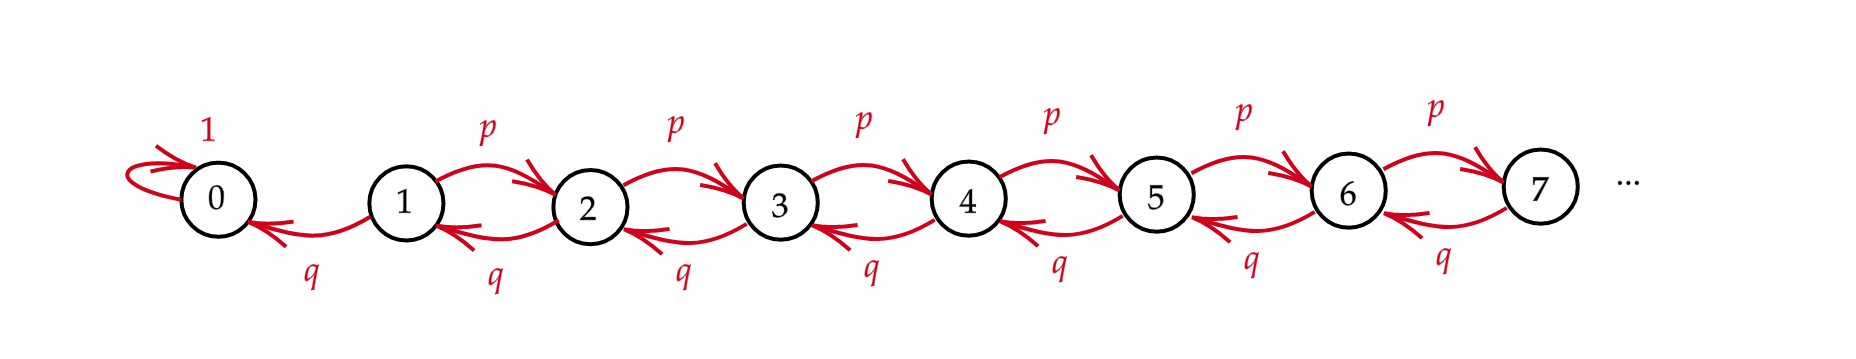
\includegraphics[width=\textwidth]{fig-27.png}
    \end{center}
    Let $(S_n)_{n \geq 0}$ be the biased random walk on $\mathbb{N}_0$ with an absorbing boundary at zero.  $(\hat{S}_n)$ is not a martingale,
    \begin{align*}
    \mathbb{E}[\hat{S}_{n+1} \mid \hat{S}_0, \cdots, \hat{S}_n]
    &= \mathbb{E}[S_{n+1} - (p - q)(n+1) \mid \hat{S}_0, \cdots, \hat{S}_n] \\
    &= \mathbb{E}[X_{n+1}] + S_n - (p - q)(n+1) \\
    &= S_n - (p - q)(n+1) + (p - q) \mathbbm{1}_{\{Y_n \neq 0\}}
    \end{align*}
    
    \noindent Define \text{$(S^{\prime}_n)_{n \geq 0}$} by \text{$S^{\prime}_n := S_n - (p - q) \cdot \min \{n, T\}$} for \text{$T := \inf \{n \mid S_n = 0\}$}. Then \text{$(S^{\prime}_n)$} is a martingale.
\end{ex}

\begin{ex}{Absorption Time for Biased Random Walk}{label}
  If \text{$p < q$}, then \text{$(S_n)$} is absorbed with probability 1, 
    \[Y_{k} \underset{k \rightarrow \infty}{\rightarrow} 0\]
  
  \noindent Therefore,
  \begin{align*}
    \mathbb{E}[S^{\prime}_0] &= \mathbb{E}[S^{\prime}_k] \\
                             &= \mathbb{E}[S_n] - \mathbb{E}[(p - q) \cdot \min \{n, T\}]
  \end{align*}
  \noindent Taking $k \rightarrow \infty$ gives the absorption time $\mathbb{E}[T] = \frac{\mathbb{E}[X_0]}{(q - p)}$.
\end{ex}

\begin{ex}{Branching Process}{label}
  Let \text{$(Z_k)_{k \geq 0}$} be a branching process with offspring distribution \text{$X = (x_1, \cdots,)$}. Put \text{$\mathbb{E}[X] = \mu$}. Then,
  \[M_k := \frac{Z_k}{\mu^k}\]
  \noindent is a martingale. Since $Z_{k+1} \sim \sum_{j=1}^{Z_k} X_j$,
  \begin{align*}
    \mathbb{E}[M_{k+1} \mid M_1, \cdots, M_k]
    &= \mathbb{E}\left[\frac{Z_{k+1}}{\mu^{k+1}} \,\middle\vert\, M_1, \cdots, M_k \right] \\
    &= \mathbb{E}\left[\frac{\sum_{j=1}^{Z_k} X_j}{\mu^k \cdot \mu} \,\middle\vert\, Z_k \right] \\
    &= \frac{1}{\mu^k \cdot \mu} \sum_{j=1}^{Z_k} \mathbb{E}[X_j] \text{ since $\mu, k$ fixed}\\
    &= \frac{1}{\mu^k \cdot \mu} \sum_{j=1}^{Z_k} \mu \\
    &= \frac{Z_k}{\mu^k} \\
    &= M_k
  \end{align*}
\end{ex}

\begin{ex}{P\'{o}lya's Urn}{label}
  If $(R_k, B_k)$ are the number of red and blue balls at time $k$.
  \[M_k := \frac{R_k}{R_k + B_k}\]
  \noindent is a martingale. Recall that,
  \begin{align*}
    &(R_k, B_k) \rightarrow (R_k, B_{k+1}) \text{ with probability } \frac{B_k}{R_0 + B_0 + k} \\
    &(R_k, B_k) \rightarrow (R_{k+1}, B_{k}) \text{ with probability } \frac{R_k}{R_0 + B_0 + k} \\
    &(B_k, k) \rightarrow (B_k, k+1) \text{ with probability } \frac{R_0 + B_0 + k - B_n}{R_0 + B_0 + k} \\
    &(B_k, k) \rightarrow (B_{k+1}, k+1) \text{ with probability } \frac{B_k}{R_0 + B_0 + k}
  \end{align*}
  Since $(M_k)$ is a Markov Chain,
  \begin{align*}
    \mathbb{E}[M_{k+1} \mid M_1, \cdots, M_k]
    &= \mathbb{E}\left[\frac{R_{k+1}}{R_{k+1} + B_{k+1}} \,\middle\vert\, (R_k, B_k) \right] \\
    &= \mathbb{E}\left[\frac{R_{k+1}}{B_0 + R_0 + k + 1} \,\middle\vert\, (R_k, B_k) \right] \\
    &= \frac{1}{B_0 + R_0 + k + 1} \cdot \mathbb{E}\left[R_{k+1} \,\middle\vert\, (R_k, B_k) \right]
    % &= \frac{1}{B_0 + R_0 + k + 1} \cdot \mathbb{E}\left[R_{k+1} \cdot \mathbbm{1}_{A_{k+1}} + R_{k+1} \cdot \mathbbm{1}_{A^c_{k+1}} \,\middle\vert\, (R_k, B_k) \right] \\
  \end{align*}
  where $A_{k+1}$ be the event that the \text{$(k+1)$}th ball is red, given that the number of red and blue balls at time $k$ are $R_k$ and $B_k$.
  \[\underbrace{P\left(R_{k+1}=R_{k}+1\right)}_{P(A_{k+1} \mid (R_k, B_k)) = \mathbb{E}\left[\mathbbm{1}_{A_{k+1}}\right]} \cdot \frac{R_{k}+1}{R_{k}+B_{k}+1}\]
  \[+\underbrace{P\left(R_{k+1}=R_{k}\right)}_{P(A^c_{k+1}\mid (R_k, B_k))=\mathbb{E}\left[\mathbbm{1}_{A^c_{k+1}}\right]} \cdot \frac{R_{k}}{R_{k}+B_{k}+1}\]
  \noindent is the desired expectation. Simplifying,
  \begin{align*}
    &=\frac{R_{k}^{2}+R_{k}+B_{k} R_{k}}{\left(R_{0}+B_{0}+k\right) \cdot \left(R_{0}+B_{0}+k+1\right)} \\
    &=\frac{R_{k} \cdot \left(R_{k}+B_{k}+1\right)}{\left(R_{k}+B_{k}\right) \cdot \left(R_{k}+B_{k}+1\right)} \\
    &=\frac{R_{k}}{R_{k}+B_{k}} \\
    &=M_k
  \end{align*}
\end{ex}

\begin{ex}{Absorption Probabilities}{label}
  Let $(Y_k)$ be a Markov chain with an absorbing state $i$. Then,
  \[M_k := P(A_i \mid Y_k)\]
  \noindent is a martingale, where $A_i$ is the event that the chain is absorbed at $i$. By the Total Conditional Law of Expectation,
  \begin{align*}
    \mathbb{E}[M_{k+1} \mid M_0, \cdots, M_k] &= \mathbb{E}[P(A_i \mid Y_{k+1}) \mid M_0, \cdots, M_k] \\
                                              &= \mathbb{E}[P(A_i \mid Y_{k+1}) \mid Y_k] \\
                                              &= \mathbb{E}[P(A_i \mid Y_{k+1}, Y_k) \mid Y_k] \\
                                              &= P(A_i \mid Y_k) \\
                                              &= M_k
  \end{align*}
  \noindent where the third inequality follows by the Markov Property.
\end{ex}

\subsection{Limit Theorems}
\begin{defn}[Bracket]
  The \textbf{bracket} of a martingale $(M_k)_{k \geq 0}$ is\footnote{This is effectively the accumulated variance of the process $(Y_k)$.},
  \[\left\langle M_{k}\right\rangle:=\sum_{n=0}^{k} \mathbb{E}\left(\left(M_{n+1}-M_{n}\right)^{2} \mid \mathcal{F}_{n}\right)\]
\end{defn}

\begin{ex}{Simple Random Walk}{label}
  We saw that the simple random walk on $\mathbb{Z}_0$ is a martingale. 
  \[(M_{n+1} - M_n)^2 = 1 \quad \text{ for all $n \in \mathbb{N}_0$}\]
  \noindent so \text{$\langle M_k \rangle = k$ for all $k \in \mathbb{N}$}.
\end{ex}

\begin{rmk}
  Let $(M_k)_{k \geq 0}$ be a martingale. Then,
  \[\mathbb{E}\left\langle M_{k}\right\rangle=\mathbb{E}[\left(M_{n+1} - M_0\right)^2]\]
\end{rmk}

\begin{proof}
  By definition,
  \begin{align*}
    \mathbb{E}\left[\left(M_{n+1}-M_{n}\right)^{2} \mid \mathcal{F}_{n}\right]
    &= \mathbb{E}\left[M_{n+1}^{2}+M_{n}^{2}-2 \cdot M_{n+1} M_{n} \mid \mathcal{F}_{n}\right] \\
    &= \mathbb{E}\left[M_{n+1}^{2} \mid \mathcal{F}_n\right]+M_n^2 + 2 \cdot M_n^2
  \end{align*}

  \noindent Therefore,
    \begin{align*}
    \mathbb{E}\left[\left\langle M_{k}\right\rangle\right]
    &=\mathbb{E}\left[\sum_{n=0}^{n} \mathbb{E}\left[\left(M_{n+1}-M_{n}\right)^{2} \mid \mathcal{F}_{n}\right]\right] \\
    &= \sum_{n=0}^{n} \mathbb{E}\left[\mathbb{E}\left[\left(M_{n+1}-M_{n}\right)^{2} \mid \mathcal{F}_{n}\right]\right] \\
    &= \sum_{n=0}^{n} \mathbb{E}\left[\mathbb{E}\left[M_{n+1}^{2} \mid \mathcal{F}_n\right]+M_n^2 - 2 \cdot M_n^2\right] \\
    &= \sum_{n=0}^{n} \mathbb{E}[M_{n+1}^{2}]+\mathbb{E}[M_n^2] - 2 \cdot \mathbb{E}[M_n^2] \\
    &= \sum_{n=0}^{n} \mathbb{E}[M_{n+1}^{2}]- \mathbb{E}[M_n^2] \\
    &= \mathbb{E}[M_{n+1}^{2}]- \mathbb{E}[M^2_0] \\
    &= \mathbb{E}[\left(M_{n+1} - M_0\right)^2]
  \end{align*}
\end{proof}

\begin{ex}{P\'{o}lya's Urn (Bracket Process)}{label}
  Since $\frac{R_{n}}{n+n_{0}\vphantom{\frac{1}{2}}} \geq \frac{R_{n}}{n+n_{0}+1 \vphantom{\frac{1}{2}}}$, we have that,
  \begin{align*}
    \mathbb{E}\left[\left(\frac{R_{n+1}}{n+1+n_{0}}-\frac{R_{n}}{n+n_{0}}\right)^{2} \,\middle\vert\, \mathcal{F}_{n}\right] &\leq \frac{1}{(n+1+n_0)^2}
  \end{align*}
  \noindent Implying that, for all $n \in \mathbb{N}$,
  \[\left\langle M_{n}\right\rangle \leq \sum_{k=1}^{\infty} \frac{1}{k^{2}}=\frac{\pi^{2}}{6}<\infty\]
\end{ex}

\begin{thm}
  Let $(M_k)_{k \geq 0}$ be a martingale. Suppose that,
  \[P\left(\sup_n \langle M_n \rangle < \infty\right) = 1\]
  \noindent Then, $\lim _{n \rightarrow \infty} M_{n}$ exists. Denote it by $M_{\infty}$. Then,
  \begin{enumerate}
    \item $P\left(\lim _{n \rightarrow \infty} M_{n}=M_{\infty}\right)=1$
    \item $\sup \mathbb{E}[\langle M_n \rangle] < \infty$
    \item $M_n = \mathbb{E}[M_{\infty} \mid \mathcal{F}_n]$
  \end{enumerate}
\end{thm}

\begin{proof}
  The proof was not given in class.
\end{proof}

\begin{thm}
  Let $(M_k)_{k \geq 0}$ be a martingale. If $M_n \geq 0$ for all $n \in \mathbb{N}$, then there exists a random variable $M_{\infty} < \infty$ such that,
  \[P\left(\lim _{n \rightarrow \infty} M_{n}=M_{\infty}\right)=1\]
\end{thm}

\begin{proof}
  The proof was not given in class.
\end{proof}

\begin{marginfigure}
      \textbf{10 Runs of the P\'{o}lya's Urn Process:}
      \begin{center}
        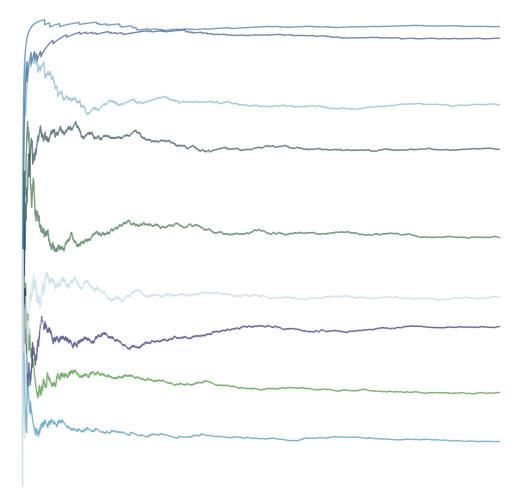
\includegraphics[width=0.9\textwidth]{fig-28.png}
        \caption{It was proven in class that, \[M_n := \frac{R_n}{n} \rightarrow M_{\infty}\] where $M_{\infty} \sim$ Unif$([0,1])$.}
      \end{center}
\end{marginfigure}

\begin{ex}{Branching Processes (Bracket Process)}{label}
  Let \text{$(M_k)_{k \geq 0}$} be the martingale for a branching process \text{$(Z_k)_{k \geq 0}$}, as defined above. Then,
  \begin{align*}
     \langle M_k \rangle
     &= \sum_{k=1}^n \mathbb{E}\left[(M_{k+1} - M_k)^2 \,\middle\vert\, \mathcal{F}_k \right] \\
     &= \sum_{k=1}^n \mathbb{E}\left[\left(\frac{Z_{k+1}}{\mu^{k+1}}-\frac{Z^k}{\mu^k}\right)^2 \,\middle\vert\, \mathcal{F}_k \right] \\
     &= \sum_{k=1}^n \mathbb{E}\left[\left(\frac{1}{\mu^{k+1}} \cdot \sum_{i=1}^{Z^k} X_i -\frac{Z^k}{\mu^k}\right)^2 \,\middle\vert\, \mathcal{F}_k \right] \\
     &= \sum_{k=1}^n \mathbb{E}\left[\frac{1}{\mu^{2k}} \cdot \left(\sum_{i=1}^{Z^k} \left(\frac{X_i}{\mu} -1\right) \right)^2 \,\middle\vert\, \mathcal{F}_k \right] \\
     &= \sum_{k=1}^n \mathbb{E}\left[\frac{1}{\mu^{2k}} \cdot \left(\sum_{i=1}^{Z^k} \left(\frac{X_i}{\mu} - \frac{\mu}{\mu}\right) \right)^2 \,\middle\vert\, \mathcal{F}_k \right] \\
     &= \sum_{k=1}^n \frac{1}{\mu^{2k}} \cdot \mathbb{E}\left[\left(\sum_{i=1}^{Z^k} \left(\frac{X_i}{\mu} - \frac{\mu}{\mu}\right) \right)^2 \,\middle\vert\, \mathcal{F}_k \right] \\
     &= \frac{Z_{n}}{\mu^{2 n}} \cdot \frac{\operatorname{Var}\left(X_{1}\right)}{\mu^{2}}
   \end{align*} 
  \noindent using the definition of the population variance. Now, we can bound $\sup \left\langle M_{n}\right\rangle$ since $\langle M_n \rangle$ is an increasing sequence,
  \[\sup \left\langle M_{n}\right\rangle \leq \sum_{k=0}^{\infty} \frac{Z_{k}}{\mu^{2 k}} \frac{\operatorname{Var}\left(X_{1}\right)}{\mu^{2}}\]
  \noindent and use the mean exponential growth rate to conclude that,
  \[\mathbb{E}\left[\sup \left\langle M_{n}\right\rangle\right] \leq \sum_{k=0}^{\infty} \mathbb{E}\left[\frac{Z_{k}}{\mu^{2 k}}\right] \frac{\operatorname{Var}\left(X_{1}\right)}{\mu^{2}} =\sum_{k=0}^{\infty} \frac{1}{\mu^{k}} \frac{\operatorname{Var}\left(X_{1}\right)}{\mu^{2}}\]
  \noindent with $\mu > 1$ and $\operatorname{Var}\left(X_{1}\right) < \infty$, the ratio $M_k$ converges to a non-degenerate limit random variable. 
\end{ex}
\end{document}
